% Williams Physics Thesis template
% Patterned after the work of Cole Meisenhelder '15
% Commented by Prof. Charlie Doret, 12/2016

\documentclass[12pt, oneside]{book} 

% The \usepackage{} command will import predefined fonts, symbols, environments, etc.  For example, the ams packages below come from the American Mathematical Society and include all kinds of useful math symbols like integrals
\usepackage{amscd}
\usepackage{amsmath}
\usepackage{amssymb}
\usepackage{amsthm}
\usepackage{verbatim}
\usepackage[utf8]{inputenc}
\usepackage{geometry}                		% See geometry.pdf to learn the layout options. There are lots.
\geometry{letterpaper}                   		% ... or a4paper or a5paper or ... 
%\geometry{landscape}                		% Activate for for rotated page geometry
\usepackage[pdftex]{graphicx}				% Use pdf, png, jpg, or eps� with pdflatex; use eps in DVI mode	
\usepackage{setspace}
\usepackage{physics}
\usepackage{subcaption}
\usepackage[numbers]{natbib}
\usepackage{pdfpages}
\usepackage{bm}

\usepackage{wrapfig}				% enables the use of \wrapfig, for figures with text wrapped around them
%\usepackage{lipsum}			% gives access to \lipsum, which dumps some latin text into your document as filler if you want to check formatting

%\usepackage[parfill]{parskip}    		% Activate to begin paragraphs with an empty line rather than an indent

\usepackage{hyperref}
\hypersetup{
	colorlinks=true, %set true if you want colored links
	linktoc=all,     %set to all if you want both sections and subsections linked
	allcolors = black %get rid of weird auto link highlighting
}
% \usepackage{sidecap}
% \usepackage[colorinlistoftodos]{todonotes}
\usepackage{fancyvrb} %useful for codeblocks not being split
\usepackage{multicol}
% \usepackage[hashEnumerators,smartEllipses]{markdown}

\usepackage{pmboxdraw}  %needed for code file tree symbols
% for code blocks -------
% \usepackage{listings}
% \usepackage{color}
% \definecolor{dkgreen}{rgb}{0,0.6,0}
% \definecolor{gray}{rgb}{0.5,0.5,0.5}
% \definecolor{mauve}{rgb}{0.58,0,0.82}
% \lstset{frame=tb,
%   language=Python,
%   aboveskip=3mm,
%   belowskip=3mm,
%   showstringspaces=false,
%   columns=flexible,
%   basicstyle={\small\ttfamily},
%   numbers=none,
%   numberstyle=\tiny\color{gray},
%   keywordstyle=\color{blue},
%   commentstyle=\color{dkgreen},
%   stringstyle=\color{mauve},
%   breaklines=true,
%   breakatwhitespace=true,
%   tabsize=3
% }
% -------

% Here we set the page dimensions to match the standard thesis format.  These values should not be changed.
%%% SET LENTGH AND WIDTH %%%
\setlength{\textwidth}{6.5in}
\setlength{\textheight}{8.5in}
\setlength{\oddsidemargin}{0pt}
\setlength{\evensidemargin}{0pt}
\setlength{\topmargin}{0pt}
\setlength{\marginparsep}{0pt}
\setlength{\marginparwidth}{1in}

%\begin{document} starts LaTeX looking for actual content.  Everything above this point is purely formatting.
\begin{document}

\begin{titlepage}
\begin{center}

% \vspace* creates some vertical white space on the page to make the title page look more pleasing.  \vspace would do much the same thing, but would not insert the white space if we were at the top of a fresh page.  As this is the start of the document we're obviously at the beginning of a page, so the asterisk is necessary to ensure we still put in two cm of white space.
\vspace*{2cm}

{\huge Investigation of Bond Strain Effects\\on XANES Spectra by \\Supervised Machine Learning} % \huge sets the font size.  Other options include things like \large, \Large, \small, \tiny, etc.

\vspace{2cm}

{\large by\\Jeremy K. Thaller}

\vspace{2cm}

%% Centered version
% \begin{multicols}{2}
% 	Professor Anatoly Frenkel, Advisor \hfill \\
% 	Brookhaven National Laboratory \hfill \\
% 	Chemistry Division \hfill \\
% 	\columnbreak
% 	Professor Wolfgang Schmahl, Advisor \\
% 	Ludwig-Maximilians-Universität München \\
% 	Fakultät Geowissenschaft
% \end{multicols}

\noindent\begin{tabular}[t]{@{}l}
	Professor Anatoly Frenkel, Advisor\\
	Brookhaven National Laboratory\\
	Chemistry Division \\
	New York, USA
\end{tabular}
\hfill
\begin{tabular}[t]{l@{}}
% \begin{tabular}[t]{r@{}}
	Professor Wolfgang Schmahl, Advisor \\
	Ludwig-Maximilians-Universität\\
	Fakultät Geowissenschaft \\
	München, Germany
\end{tabular}

% \vfill creates an arbitrary amount of vertical white space as necessary to fill the page
\vfill

A Master thesis submitted to the Faculty
of Earth- and Environmental Sciences\\
of Ludwig-Maximilians-Universität München
in the framework of MaMaSELF

\vspace*{3cm}

% Brookhaven National Labs\\
% Brookhaven, New York\\
\today % you might choose to set a permanent date, but \today will put in today's date
\end{center}
\end{titlepage}

% \frontmatter defines the pieces of the thesis which will use roman numerals for page numbering
\frontmatter 


% \chapter{} and/or \chapter*{} will create a chapter in your thesis.  Including the asterisk will cause the chapter to not appear in the table of contents.

% \input will reference a particular .tex file.  Here we are grabbing a file entitled Abstract stored in the folder Chapters
\chapter{Abstract}
% Here is where you'll include the actual text for your abstract.  Because this lives inside the main document and will be included with a \input command, no tags are needed to start a new document.  Instead, just type.


% Your abstract will summarize your thesis in one or two paragraphs.  This brief summary should emphasize methods and results, not introductory material.

% X-ray absorption spectroscopy (XAS) is a widely used experimental technique for material characterization. The two
A recently published method \cite{Timoshenko2017} enables the decoding of X-ray absorption near edge structure (XANES) spectra of nanoparticles to obtain important structural descriptors: coordination numbers and bond distances. Utilizing supervised machine learning (ML), the method trains an artificial neural network (ANN) to recognize a relationship between the nanoparticle structure and the XANES spectrum. Once trained, the ANN is used to ``invert'' an unknown spectrum to obtain the corresponding descriptors of the catalyst structure. Bond strain is known to be an important catalytic descriptor, yet, its accurate determination in reaction conditions is hampered by high temperature and low weight loading of real catalysts. ML–assisted XANES analysis offers a promising new direction for extracting the bond strain information from XANES---and not from extended x-ray absorption fine structure (EXAFS) analysis. Using simulated XANES spectra of Au nanoparticles, we have developed an ANN capable of ``inverting'' an unseen XANES spectrum and predicting structural disorder in the form of mean-squared displacement. The utility of the method was demonstrated on computer-simulated nanoparticles of degrees of disorder. Further work to test the model onto particles of varying sizes and bridge the model's predictive domain onto experimental absorption spectra is required.

% Further, the network is being trained to predict additional disorder descriptors, which would allow for the reconstruction of the radial distribution function, $g(r)$. This prediction is possible in part due to a new statistical averaging approach whereby XANES spectra of disordered structures are created from simulated XANES spectra of non-disordered structures.

% https://www.worldscientific.com/doi/abs/10.1142/9789811204579_0007
% Y. Lin, M. Topsakal, J. Timoshenko, D. Lu, S. Yoo, A. I. Frenkel
% Machine-Learning assisted structure determination of metallic nanoparticles: A benchmark
% In: Handbook on Big Data and Machine Learning in the Physical Sciences, World Scientific Series on Emerging Technologies, v.2, Chapter 7, pp. 127-140 (2020).
\chapter{Executive Summary}
% Here we have your executive summary.

Your executive summary will give a detailed summary of your thesis, hitting the high points and perhaps including a figure or two.  This should have all of the important take-home messages; though details will of course be left for the thesis itself, here you should give enough detail for a reader to have a good idea of the content of the full document.  Importantly, this summary should be able to stand alone, separate from the rest of the document, so although you will be emphasizing the key results of your work, you will probably also want to include a sentence or two of introduction and context for the work you have done.

\begin{figure}[h!]
    \centering
    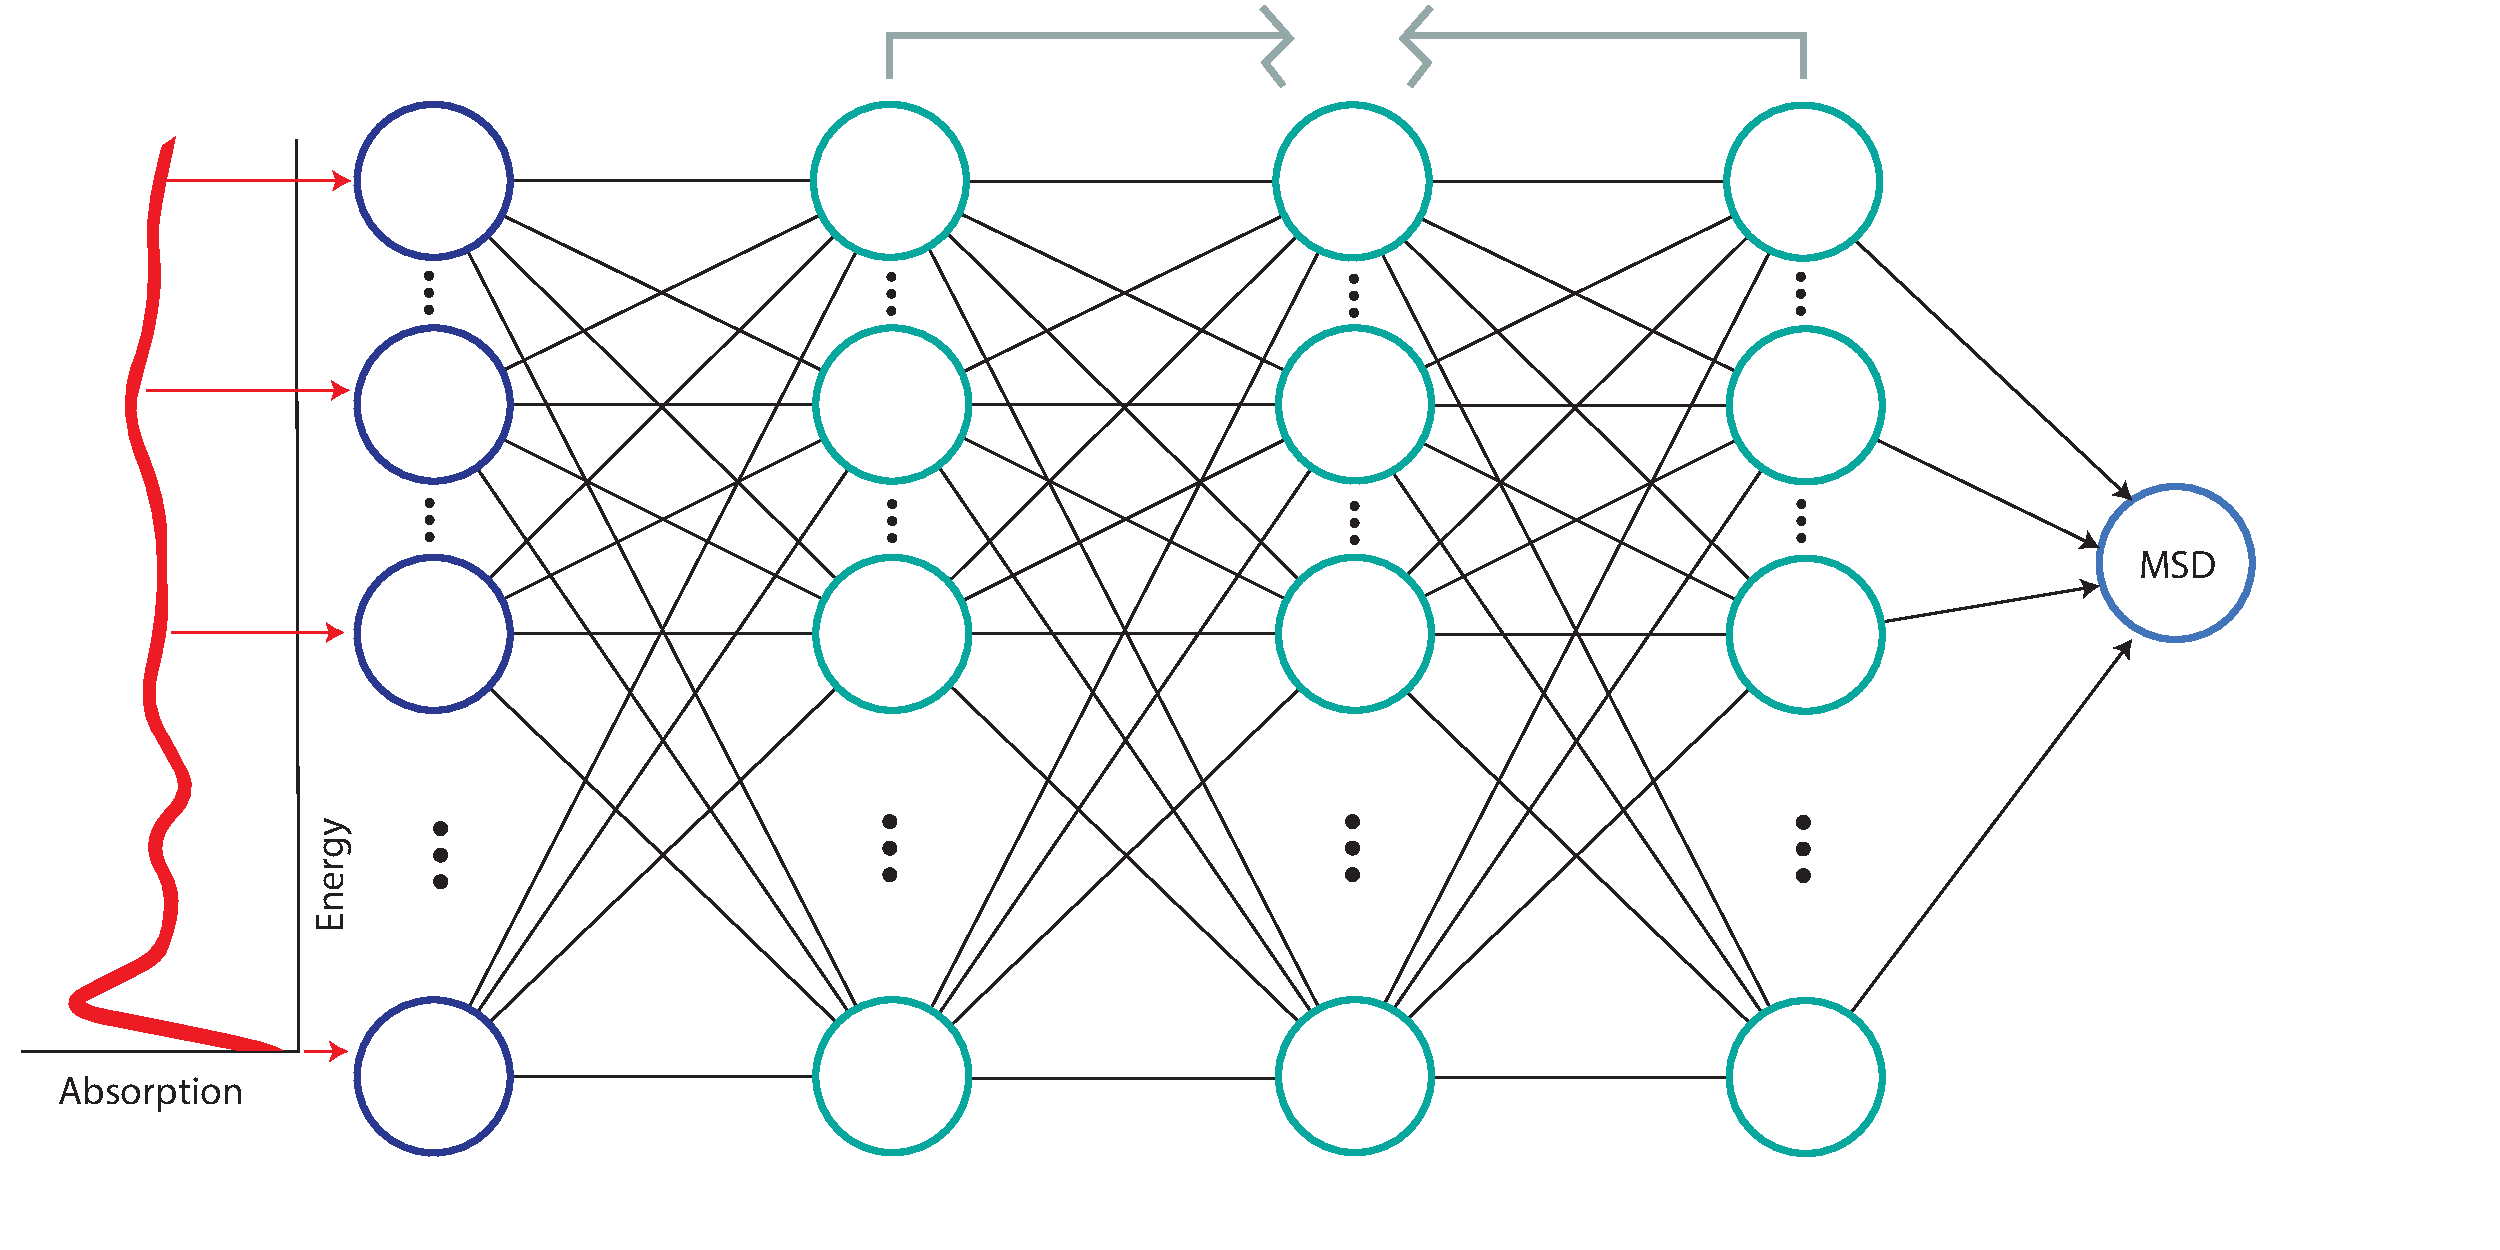
\includegraphics[width=\linewidth]{Chapters/Figures/thesis-design.pdf}
    \caption[Project Approach]{Thesis design}
\end{figure}


\chapter{Acknowledgments}
% Here we have a section where you might choose to acknoweldge your family, fellow students, advisor, dog, etc.

I would like to thank my advisor Professor Anatoly Frenkel and my professors in Germany and Poland over the past two years. I also owe a great debt of gratitude towards those who took the time to help proofread my work, as well as the free and open-source software (FOSS) community.

%\tableofcontents will create a table of contents.  By default it will include entries for any \chapter, \section, and \subsection command that appears in your thesis unless you have called the tag with an asterisk
\tableofcontents

\listoffigures

% \mainmatter defines the main body of the thesis and marks where regular numbering will begin
\mainmatter

\chapter{Introduction}
% Look!  A mock introduction

The introduction is one of the most important pieces of your thesis.  Here is a place for you to introduce the problem(s) on which you have worked and place them in the larger context of your field.  You should aim to ensure that this section is completely understandable to virtually anyone - and certainly anyone with a sophomore-level grasp of physics.  Presumably, this will include references to the literature.

In addition to setting your work into context, a second good idea for your introduction is to give a short outline for what the rest of your thesis will discuss.  This is often done in the closing paragraph(s) of the introduction with sentences like ``In the following chapters \ldots " and ``Chapter 2 discusses \ldots"  Tremendous detail is not required in this outline, but rather just a brief road map for the rest of the document.

\section{X-ray Absorption Spectroscopy}
\emph{I want to describe the problem we're trying to solve in this section. So I want to motivate the problem by describing XAFS a little so I can describe the limitations of XANES and why this project is useful. More in-depth explanations can be placed in chapter 2}

\subsection{EXAFS}
Extended X-ray Absorption Fine Structure (EXAFS)

\subsection{XAFS}
X-ray Absorption Fine-Structure spectroscopy, or XAFS, refers to the study of absorption spectra created from high-intensity x-ray interactions.

Probably want to talk about these papers in this section \cite{timoshenko2018neural} \cite{Timoshenko2017}.



% \chapter{XAFS In Depth}
\chapter{Simulating Disorder}
% % Chapter 2: XAFS Simulations
% % Chapter 2: XANES
% \textit{In this section, I can write about XANES to a super in-depth extent, and likely the bulk of this chapter will be about FEFF and FDMNES theoretical calculations}
% \section{Maybe derivation of EXAFS Equation}
% \section{FEFF vs. FDMNES Approaches}
% \section{Theoretical XANES Calculations}
% -------------------------------------------------------------

Before making any predictions, neural networks must first be trained on a large quantity of data. Specifically, to teach our neural network to predict the mean squared displacement (MSD), we must first generate a large quantity of training data comprised of XANES spectra, each labeled with a known MSD. Gathering such a large quantity of high-quality experimental data would be impractically time-intensitive and expensive. Rather, simulations provide a practical alternative, though even simulating each possible disordered structure individually, would be extremely time-intensive. This process is discussed in section \ref{sec:traditional-disorder}. First, a discussion on the development of a new method for simulating disordered nanoparticles is presented in sections \ref{sec:start-disorder}--\ref{sec:end-disorder}. The new process utilizes the statistical averaging of non-disordered structures. Instead of simulating hundreds of defined, disordered structures, we run many XANES simulations of simple, non-disordered structures and generate the disordered spectra via clever statistical averaging. In this chapter, we explain this statistical weighting process in-depth, beginning with the creation of simple, non-disordered spectra for the FEFF input files and culminating in the creation of many possible disordered spectra with known MSDs. The efficacy and limitations of this approach are discussed in section \ref{sec:pa-feff-vs-gaussian-feff}.

\section{Generating Distortion Not Disorder} \label{sec:start-disorder}
Instead of creating structures with a range of \textit{disorder}, we instead begin by generating structures with a range of \textit{distortion}. Wheres \textit{disorder} refers to a statistical average of atomic displacement from their original position, characterized by MSD and the width $ \sigma^2 $ of a partial radial distribution function, \textit{distortion} refers only to isotropic expansion or contraction of the subject. Equivalently, we define distortion as a radial shift in all atomic positions away from (or towards) the center atomic absorber.

% Figure created in distortion-visualizations.ipynb 
\begin{figure}[h]
	\centering
	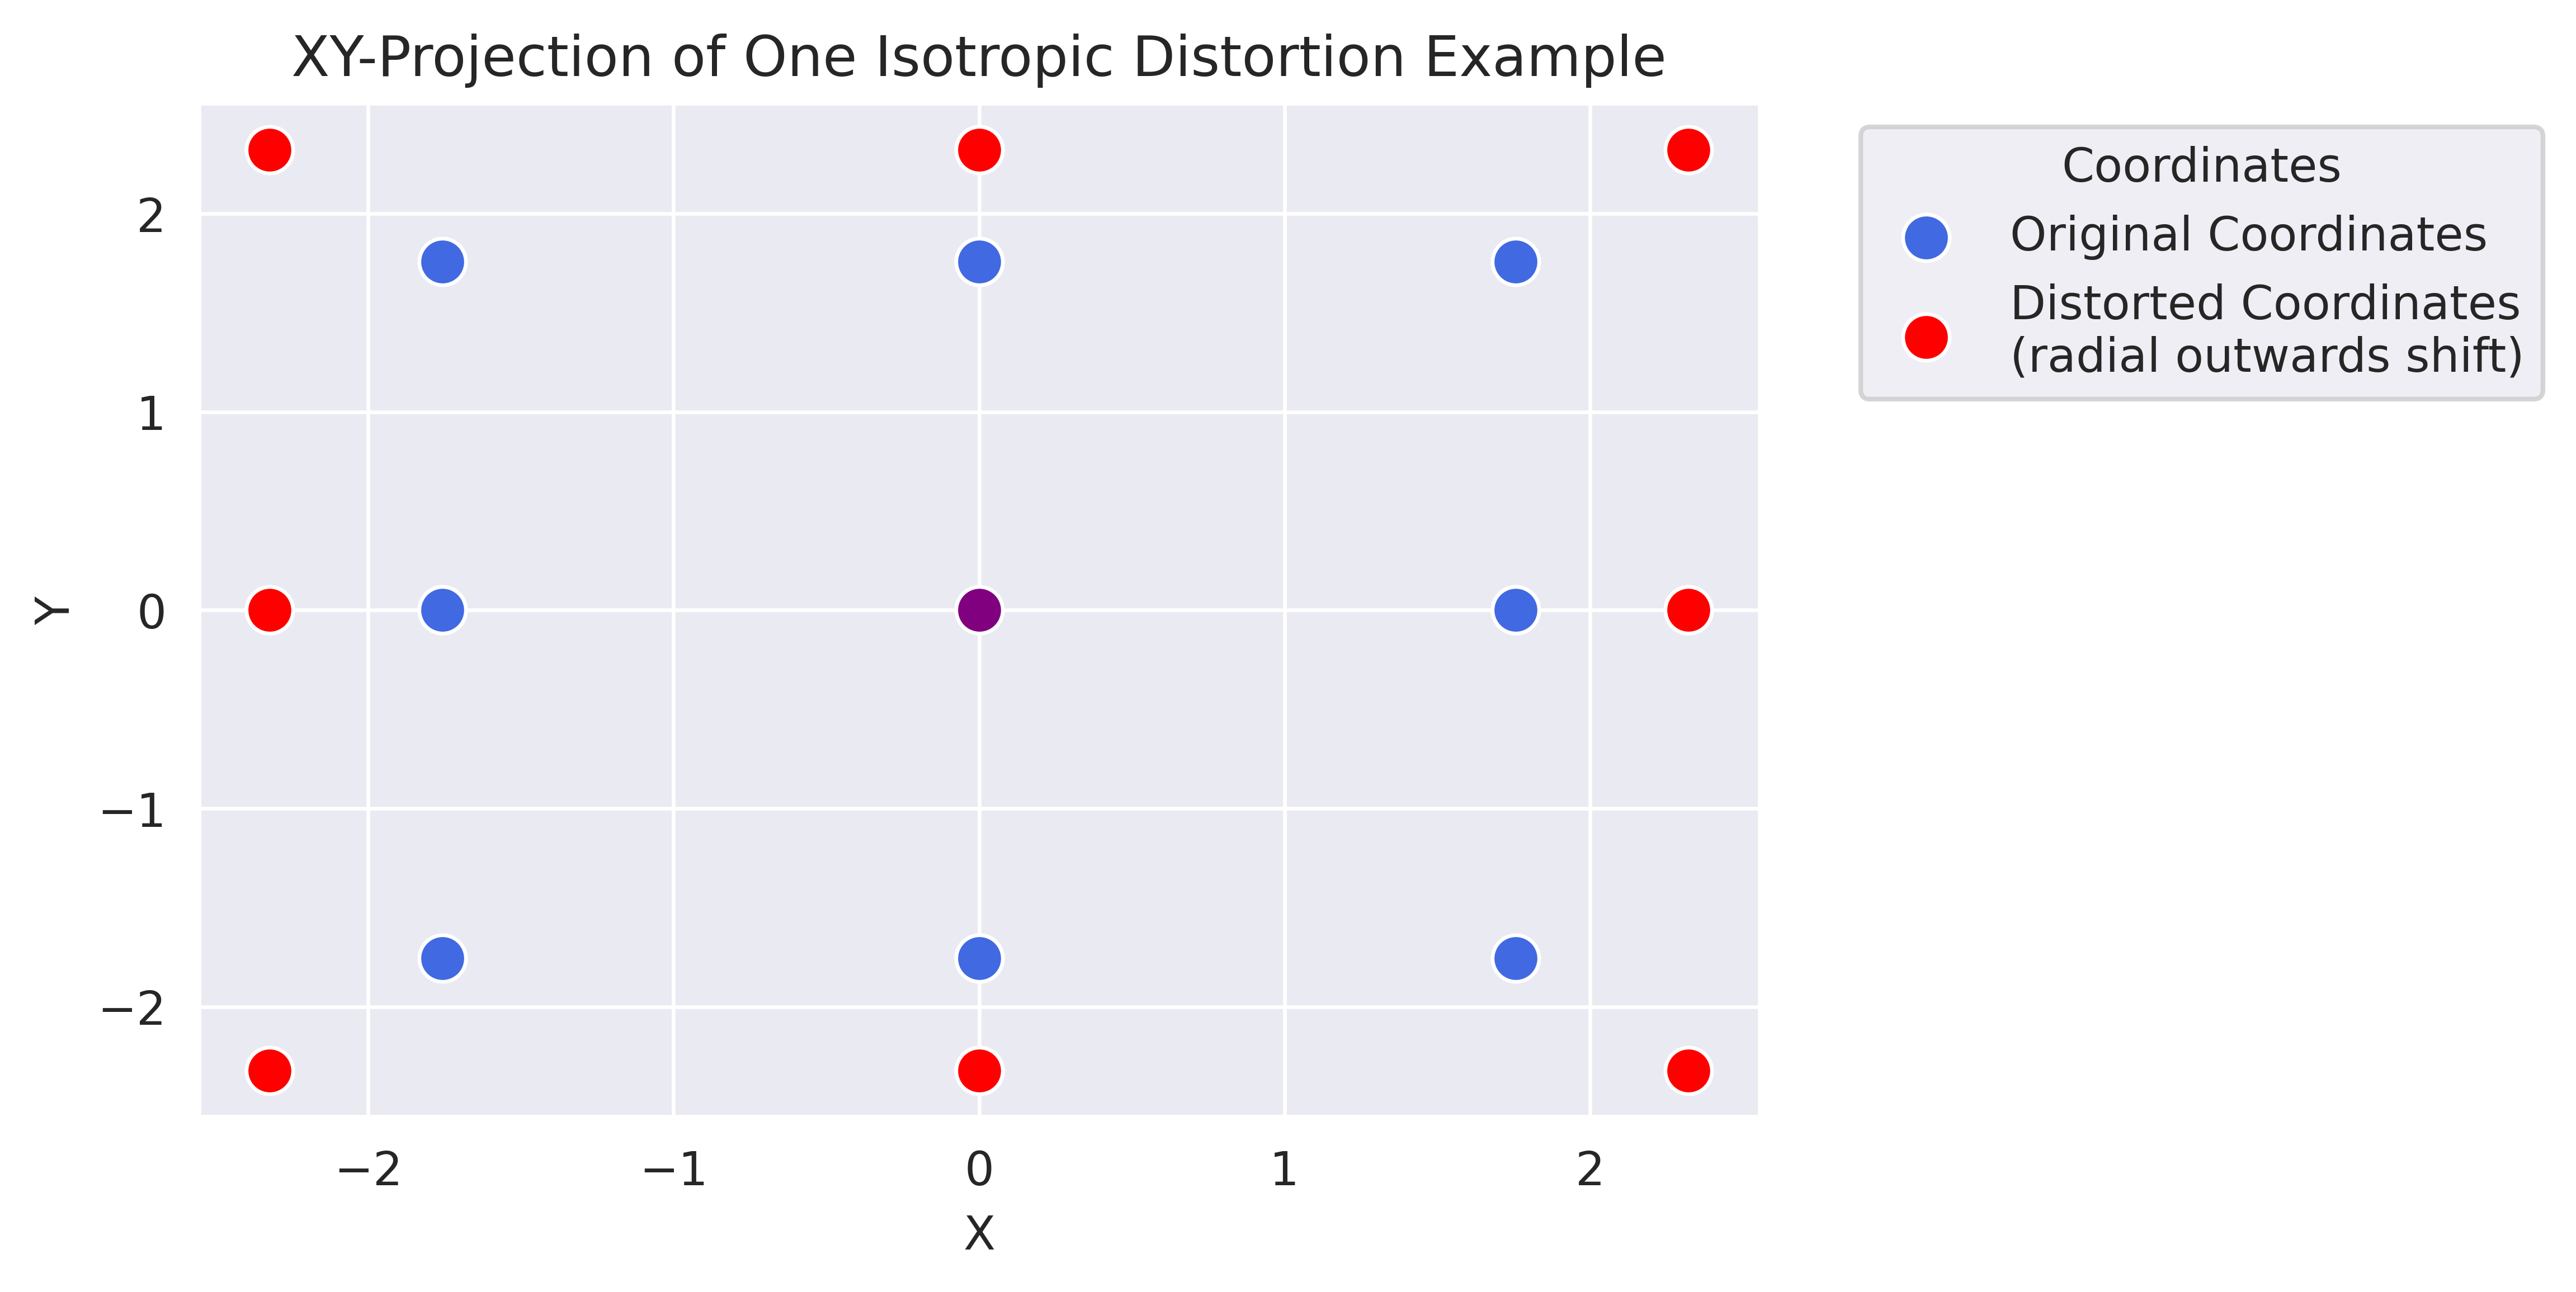
\includegraphics[width=\linewidth]{Chapters/Figures/2d_distortion_example.png}
	\caption[2D Distortion]{Each point represents an atom of first 12 nearest neighbors of a Au cluster projected onto the $xy$\nobreakdash-plane. The four corner points actually represent two atoms because of the projection. The blue atoms represent the original coordinates, and the red atoms represent the radially shifted coordinates. The center absorber atom is purple since its original position is the same as its distorted position.}
	\label{fig:2d-distortion}
\end{figure}

A 2-dimensional projection of this isotropic distortion is presented in Figure \ref{fig:2d-distortion}. Though the figure only shows the $xy$\nobreakdash-plane projection of the first 12 nearest neighbors, the actual structure used consists of the first four shells (561 atoms) with a lattice constant of 4.0782~\AA~to match that of bulk Au.\textit{Citation? Wolfram Element Data?} In reality, the nearest-neighbor distances for Au nanoparticles are likely smaller \textit{gold-lattice-const}; this can be accounted for later on in the averaging process since the original coordinates will only be one structure out of many. The important part is that the crystal structure is correct. 

We generate a total of 91 FEFF input files with different levels of distortion. Each file contains the same center absorber located at $ (0,0,0) $, but all other first shell atomic coordinates are in a shifted location on the range of $ -0.45 $~\AA~to~$ +0.45 $~\AA~in increments of $ 0.01 $~\AA. For example, the FEFF input file with the greatest inward shift has all first nearest neighbor atoms shifted $ 0.45 $~\AA~radially inwards towards the center absorber, and the FEFF input file with the largest outwards shift has the first nearest neighbor coordinates shifted $ 0.45 $~\AA~radially outwards away from the center absorber. The atoms in the outer shells are scaled accordingly to preserve the crystal structure according to:

\begin{equation}
	\label{eq:distortionator}
	\vb*{\rho}_{shifted} = \dfrac{\vb*{\rho} * \vert \vb*{\rho} \vert_{min} + \delta}{\vert \vb*{\rho} \vert_{min}} 
\end{equation}
% alpha = (df[df.rho > 0].rho.min() + delta)/df[df.rho > 0].rho.min()
% df_temp['rho'] *= alpha

\begin{minipage}{\linewidth}
Each FEFF input file is run with the following parameters: 
\begin{Verbatim}[samepage=true, numbers=left]
    SCF 4.6 0 30 .5 1
    EDGE    L3
    EXCHANGE    5   0.2 0.5
    S02 1.
    XANES   3.7 0.05    0.1
    FMS 7

    POTENTIALS
    0	79	Au	-1	-1	0.
    1	79	Au	-1	-1	0.
\end{Verbatim}
~
\end{minipage}

Running the 91 simulations (one for each of the distorted structure) takes approximately 30 minutues. Were we to generate thousands more or employ RMC or MD, this process could take weeks of compute time. We plot the resulting XANES spectra from the FEFF simulations in figure \ref{fig:feff-results}.

\begin{figure}[h]
	\centering
    \makebox[\textwidth][c]{
	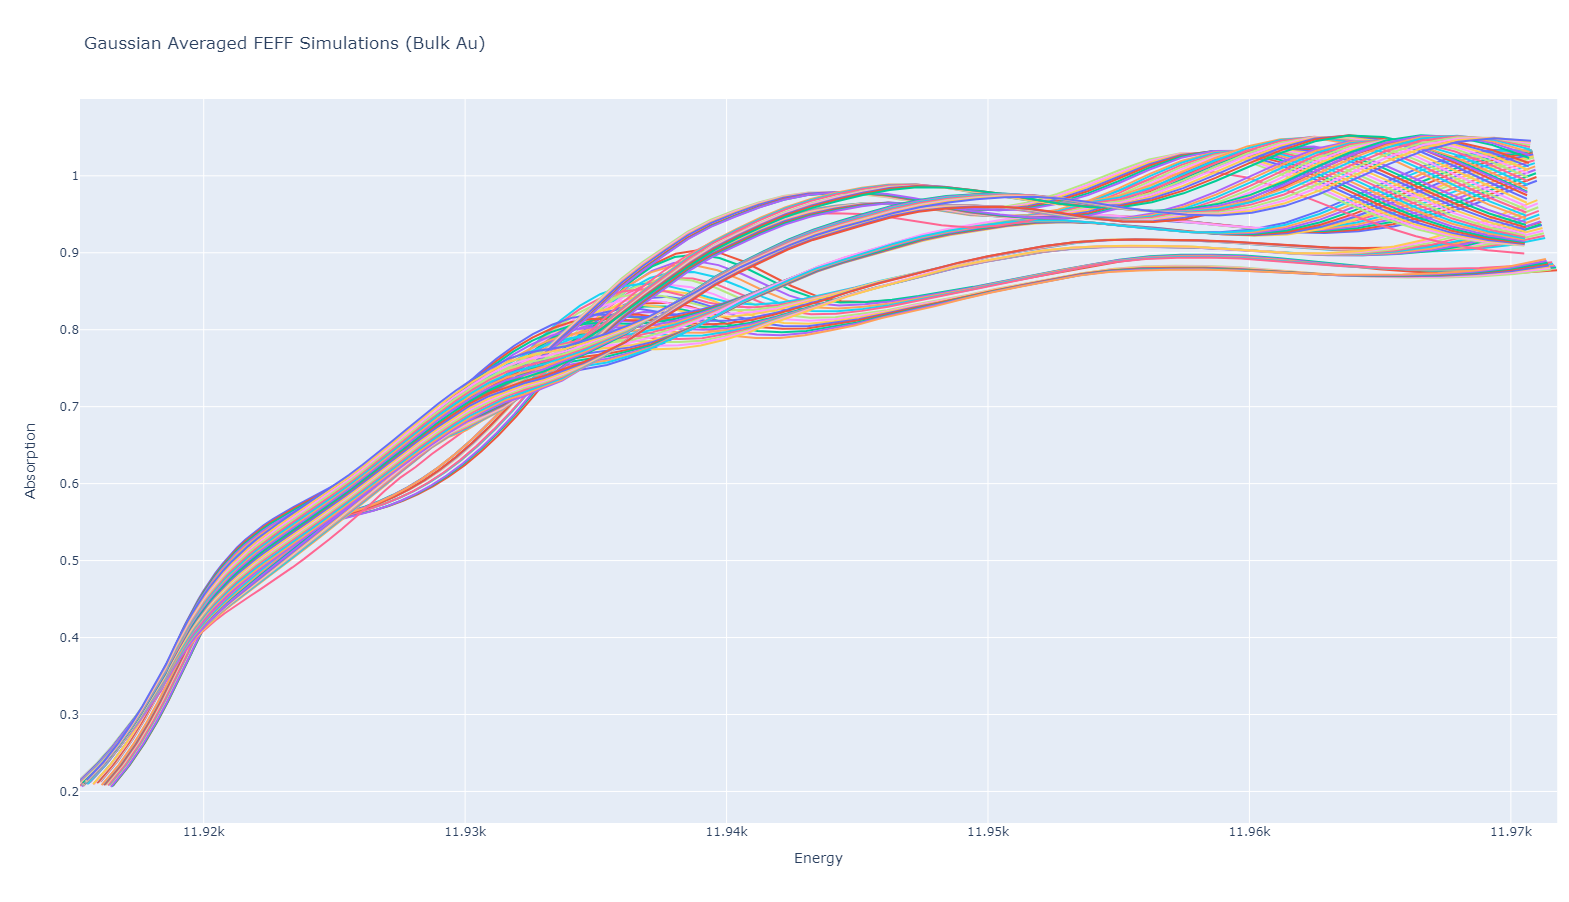
\includegraphics[width=1.1\linewidth]{Chapters/Figures/newplot.png}}
	\caption[FEFF Simulations Results]{\textit{TEMPORARY - way too much info. I'll select a few. }Each spectrum represents the FEFF simulation results for a different distorted structure. For each spectrum, the crystal structure and center absorber remain constant, the only parameter that varies is the euclidean distance from the center to the other coordinates.}
	\label{fig:feff-results}
\end{figure}

\section{Generating Disorder via Probability Distribution Averaging}

One way to characterize system disorder is with the Gaussian width, $ \sigma $ , of the partial radial distribution function. The idea of our statistical averaging method is to emulate this width by weighting the simulated XANES spectra accordingly. For example, Figure \ref{fig:gaussian-weighting-hist} depicts a histogram with $ \sigma=0.1 $~\AA. Each histogram bin represents a simulated XANES spectrum with a different isotropic displacement. For example, the bin at $ \Delta\rho=0.0 $~\AA~represents the simulated XANES spectrum with no distortion, and the bin at $ \Delta\rho=-0.2 $~\AA~represents the simulated XANES spectrum with all the atomic coordinates shifted isotropically inwards towards the center absorber by $ 0.2 $~\AA. The height of each bin, $ f(\Delta\rho) $, represents the relative contribution of each simulated XANES spectrum towards the resulting weighted spectrum. For visual clarity, Figure \ref{fig:gaussian-weighting-hist} depicts only 40 bins; the actual weighting includes 91 bins ranging from $ -0.45 $~\AA~to~$ +0.45 $~\AA.
% figure created in playground.ipynb
% !htb
\begin{figure}[h!]
	\centering
	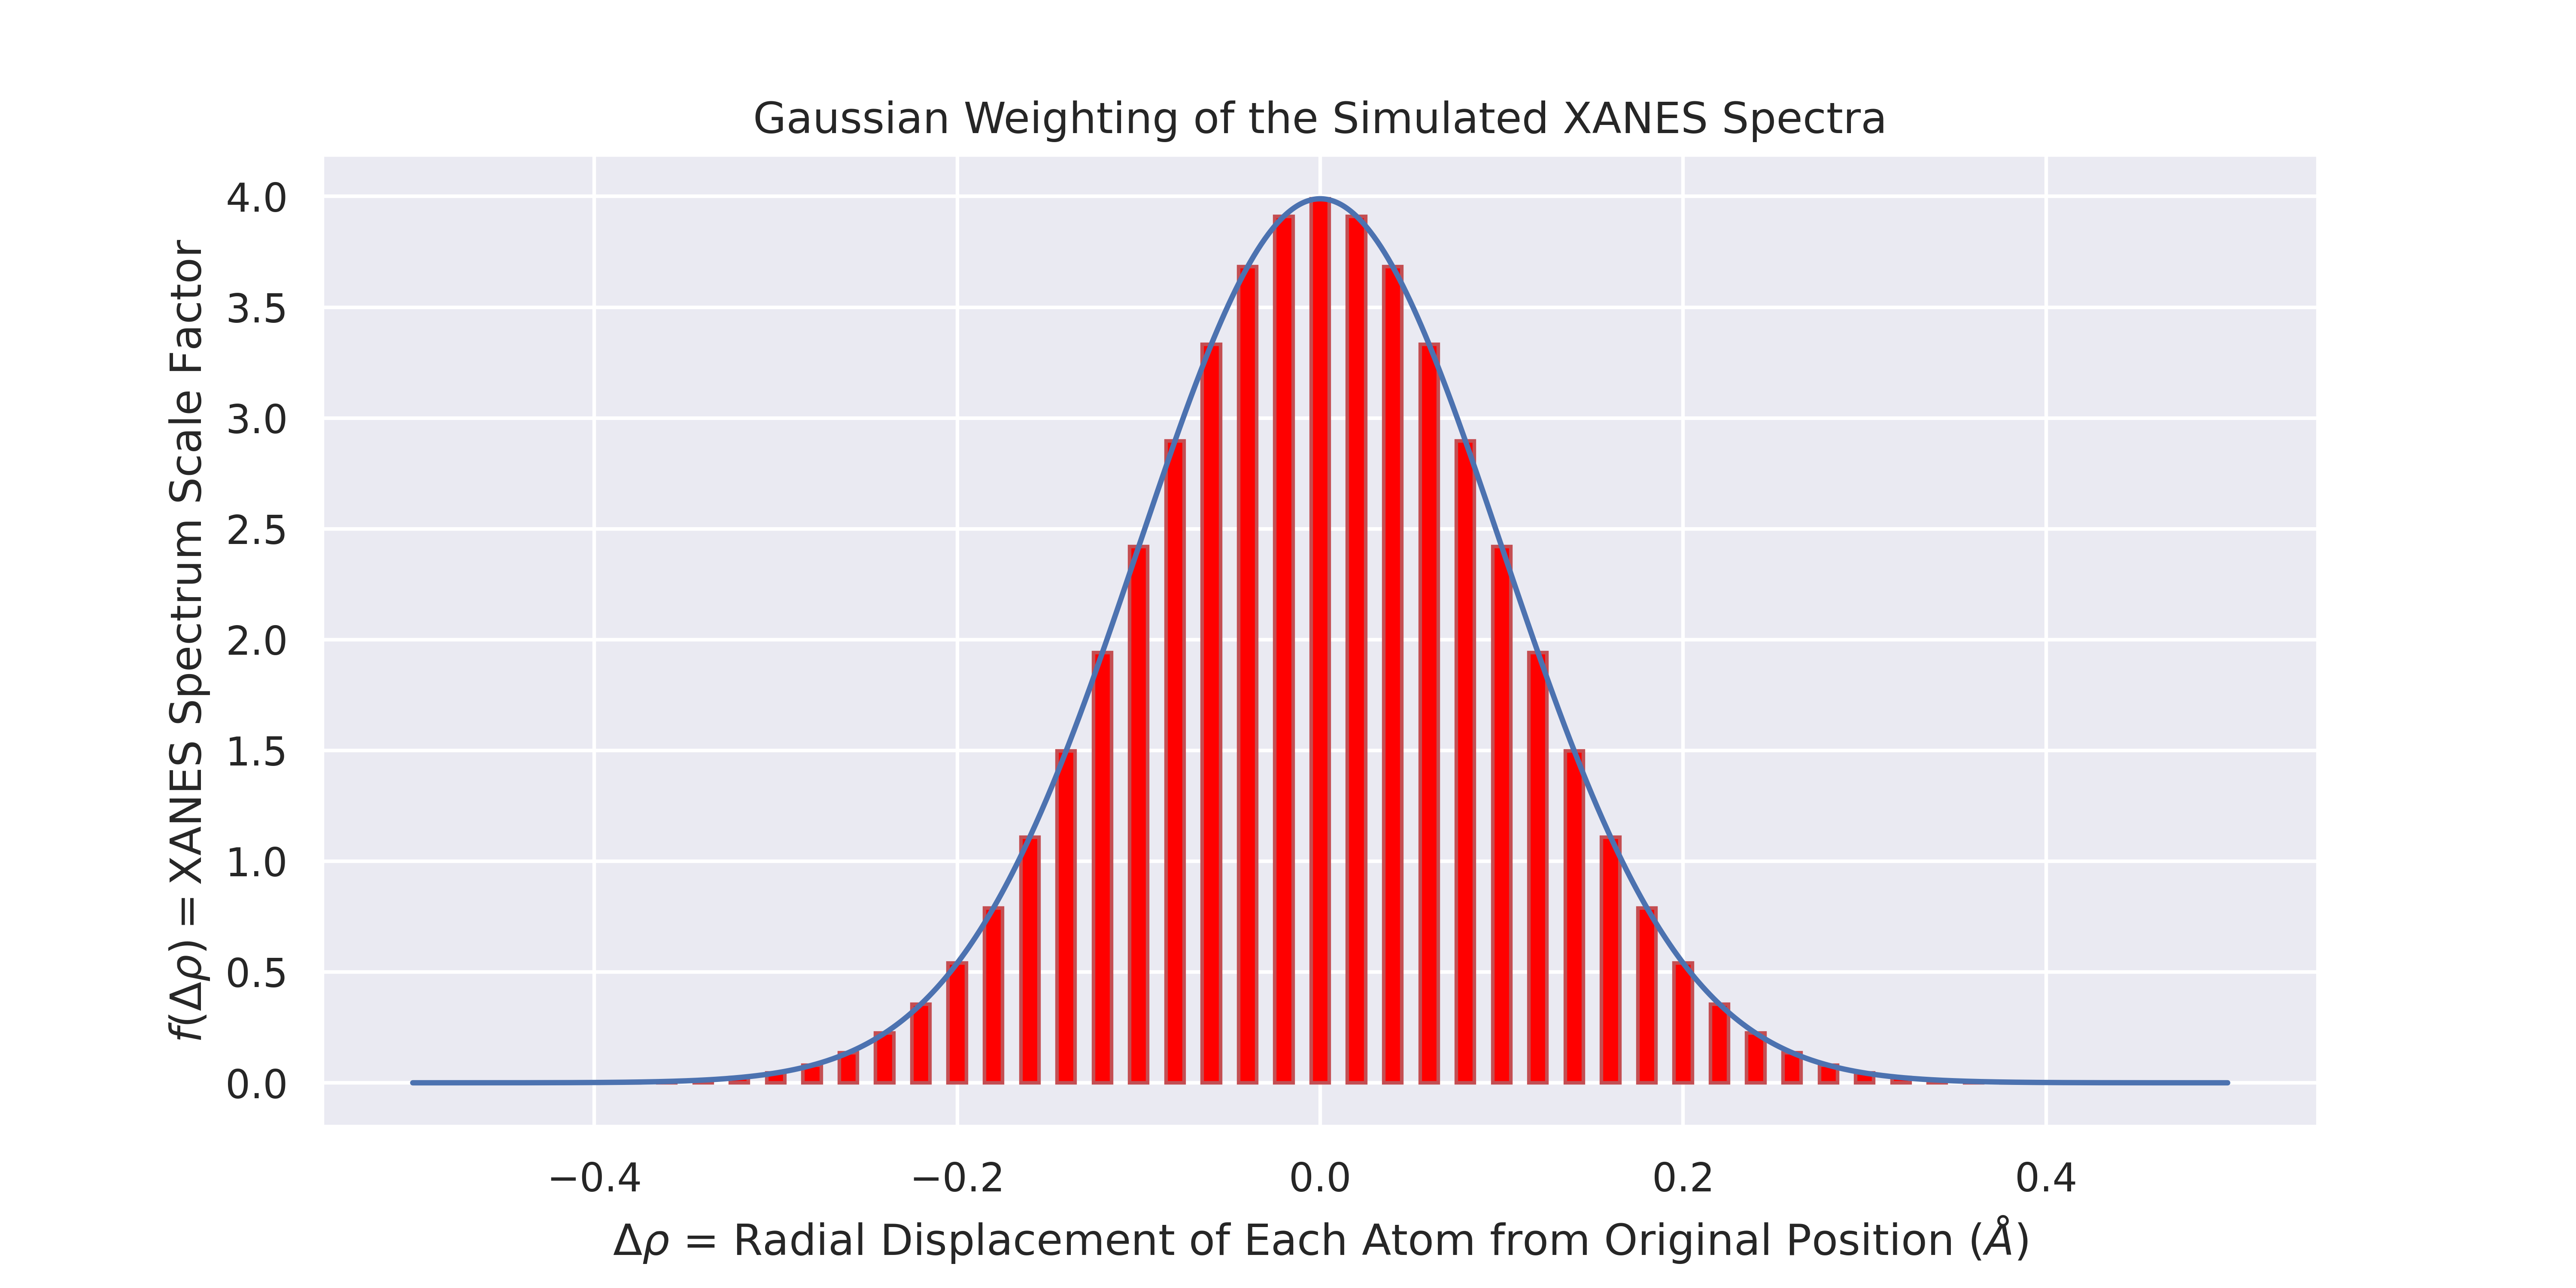
\includegraphics[width=\linewidth]{Chapters/Figures/gaussian-weighting-hist.png}
	\caption[Simulated Spectrum Gaussian Weighting]{A Gaussian distribution probability density function can be used to calculate the relative weight of each FEFF generated XANES spectrum towards one simulated, disordered spectrum. Each bin (red bar) represents a FEFF generated spectrum; the $x$-axis is the isotropic shift of the atomic positions, and the $y$-axis is the relative weight factor.}
	\label{fig:gaussian-weighting-hist}
\end{figure}

The disordered, gaussian-averaged XANES spectrum, $ \left\langle \mu(E) \right\rangle $, using the histogram weighting of the gaussian in Figure \ref{fig:gaussian-weighting-hist} is calculate via Equation (\ref{eqn:gaussian-averaging}):

\begin{equation}
	\label{eqn:gaussian-averaging}
	\left\langle \mu(E) \right\rangle  = \frac{1}{S} \sum_{\Delta\rho=-.45}^{+.45} g\left(\Delta \rho \mid \mu=0, \sigma=0.1\right) \mu(E \mid \Delta\rho)
\end{equation}

\noindent
In the above equation, $ \Delta\rho $ is the isotropic, radial displacement of each atom from its original position, and $ \mu(E \mid \Delta\rho) $ is the simulated FEFF spectrum for the given $ \Delta\rho $ configuration. Furthermore, in Equation (\ref{eqn:gaussian-averaging}), $ S $ represents a standardization factor needed to negate the effect of the changing Gaussian height as a function of the variance, $ \sigma^2 $. With the inclusion of $ S $ , only the relative heights of each bin matters for producing the averaged XANES spectrum. This standardization factor is defined in Eqation (\ref{eqn:gaussian-standardization}):

\begin{equation}
	\label{eqn:gaussian-standardization}
	S = \sum_{\Delta\rho=-.45}^{+.45} g\left(\Delta \rho \mid \mu=0, \sigma=0.01\right)
\end{equation}

\noindent
In both equations (\ref{eqn:gaussian-averaging}) and (\ref{eqn:gaussian-standardization}), the function $ g $ is just the typical Gaussian distribution probability density function (Equation \ref{eqn:gaussian}): 

\begin{equation}
	\label{eqn:gaussian}
	g(x) = \frac{1}{{\sigma \sqrt {2\pi } }}e^{{{ - \left( {x - \mu } \right)^2 } \mathord{\left/ {\vphantom {{ - \left( {x - \mu } \right)^2 } {2\sigma ^2 }}} \right. \kern-\nulldelimiterspace} {2\sigma ^2 }}}
\end{equation}

The above example only generates one (simulated) disordered XANES spectrum and does so via weighting of a Gaussian distribution with mean and variance equal to $ 0 $ and $ 0.01 $, respectively. To simulate systems with different degrees of disorder, we can vary the shape of the probability density function. With a Gaussian distribution, we can only vary the mean and variance; to simulate even more conditions, however, we can instead use the multivariate skew-normal distribution (\ref{eqn:skew-norm}) \cite{skewnorm_Azzalini_1999, 2020SciPy-NMeth}, \textit{f(x)}.

\begin{equation}
	\label{eqn:skew-norm}
	f(x)=2\phi (x)\Phi (\alpha x)
\end{equation}
 
\noindent
where $ \phi(x) $ is the Gaussian PDF:
\begin{equation}
	\label{eqn:skew-norm-pdf}
	\phi (x)={\frac  {1}{{\sqrt  {2\pi }}}}e^{{-{\frac  {x^{2}}{2}}}}
\end{equation}

\noindent
and $ \Phi (x) $ is the Gaussian CDF:
\begin{equation}
	\label{eqn:skew-norm-cdf}
	\Phi (x)=\int _{{-\infty }}^{{x}}\phi (t)\ dt
\end{equation}

%------------WIKIPEDIA EQUATION VERSION -------------
% \begin{equation}
% 	\label{eqn:skew-norm-cdf}
% 	\Phi (x)=\int _{{-\infty }}^{{x}}\phi (t)\ dt={\frac  {1}{2}}\left[1+\operatorname {erf}\left({\frac  {x}{{\sqrt  {2}}}}\right)\right]
% \end{equation}
% \noindent
% and erf is Gauss' error-function

% \begin{equation}
% 	\label{eqn:skew-norm-cdf-erf}
% 	{\displaystyle \operatorname {erf} \left(z\right)={\frac {2}{\sqrt {\pi }}}\int _{0}^{z}e^{-t^{2}}\,dt}
% \end{equation}

\noindent
Equation (\ref{eqn:skew-norm}) includes the shape parameter, $ \alpha $, which has the nice property of producing a right-skewed distribution when positive and a left-skewed distibution when negative. When $ \alpha=0 $, the distribution simply produces the typical Gaussian distribution (eq. \ref{eqn:gaussian}). Utilizing equation (\ref{eqn:skew-norm}), we can vary $ \mu, \sigma,  $ and $ \alpha $ to alter the first four moments of the function: mean, standard deviation, skew, and kurtosis. Eighteen possible skew-norm weighting functions are plotted in Figure \ref{fig:skew-norm-options}. To produce the neural network training data, 1000 such weightings are used.

\begin{figure}[h!]
	\centering
	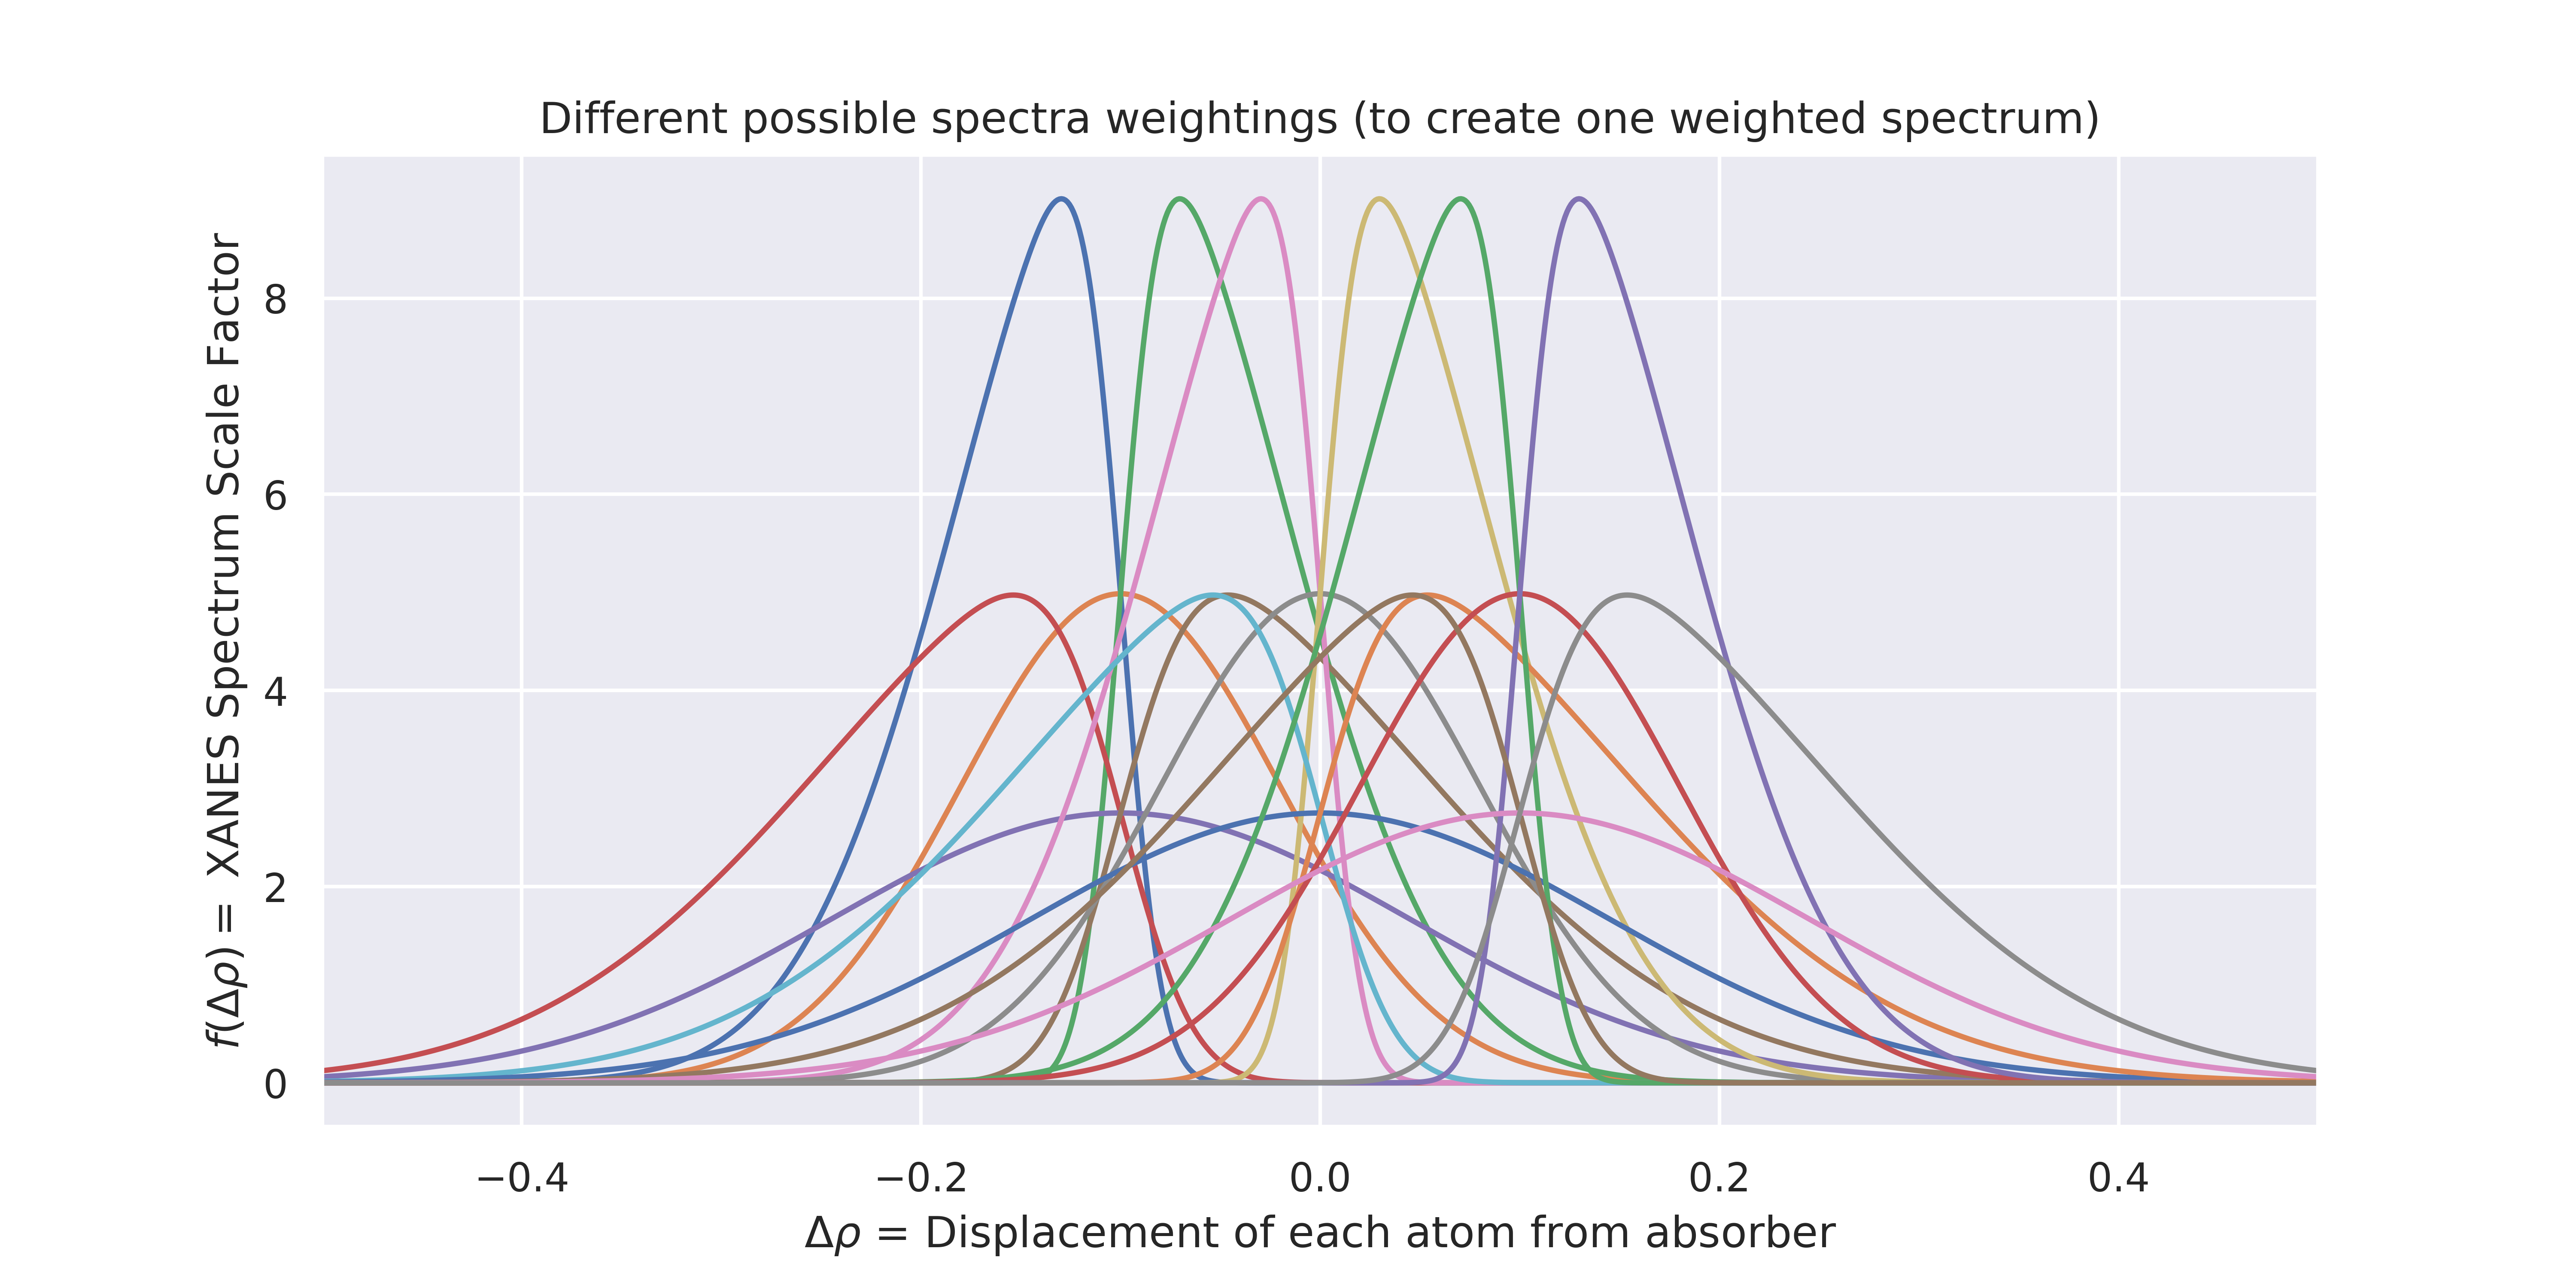
\includegraphics[width=\linewidth]{Chapters/Figures/skewnorm_options.png}
	\caption[Simulated Disordered Spectrum Weightings]{Eighteen skew-norm distributions plotted with all possible combinations of $ \sigma=\{.08, .145\} $, $ \mu=\{-.1, 0, .1\} $, and $ \alpha=\{-5,0,5\} $. Each represents a possible way to produce a simulated, disordered spectrum from many FEFF-simulated, distorted spectra} 
	\label{fig:skew-norm-options}
\end{figure}

The disorder of the skew-norm generated, disordered spectrum is characterized by the mean squared displacement of each atom from its original position ($ \Delta\rho $ ), weighted in the same manner as the spectra. \textit{Instead of characterizing the disordered spectrum by the standard deviation of the gaussian used to create it.} The weighted mean squared displacement, $ MSD $, is calculated via equation (\ref{eqn:weighted-MSD}):

\begin{equation}
	\label{eqn:weighted-MSD}
	MSD  = \frac{1}{S} \sum_{\Delta\rho=-.45}^{+.45} f\left(\Delta \rho \mid \mu, \sigma^2, \alpha \right) 
\end{equation}

\noindent
Here, $ f(x) $ is the skew-norm function from equation (\ref{eqn:skew-norm}), and the $ MSD $  of each individual FEFF spectrum is equal to the isotropic distortion, $ \Delta\rho $.  

\section{Simulation vs. Experimental Data} \label{sec:end-disorder}

To check our FEFF simulation parameters, as well as the validity of the gaussian-weighted disorder technique, we compare the simulation data to experimental data. \textit{Can someone give me citations for these?} In Figure \ref{fig:avg-experimental-vs-simulation}, both experimental and simulation spectra for bulk-like and nanoparticle scenarios are plotted. EXAFS fitting was used to characterize the disorder in the experimental measurements. For the bulk foil, this parameter was found to be $ \sigma^2=0.0081(5)~$ {\AA}$ ^2 $, and for the 8~nm disordered particle, $ \sigma^2=0.0102(8) $~{\AA}$ ^2 $.  One simulated, disordered spectrum was weighted according to the gaussian $ N(0, 0.09) $ to represent the disordered nanoparticle, and the other was weighted according to the gaussian $ N(0, 0.038)  $ to represent the bulk. These weightings correspond to $ MSD $ values that match the measured $ \sigma^2 $ values for the experimental data.  

\begin{figure}[h]
	\centering
	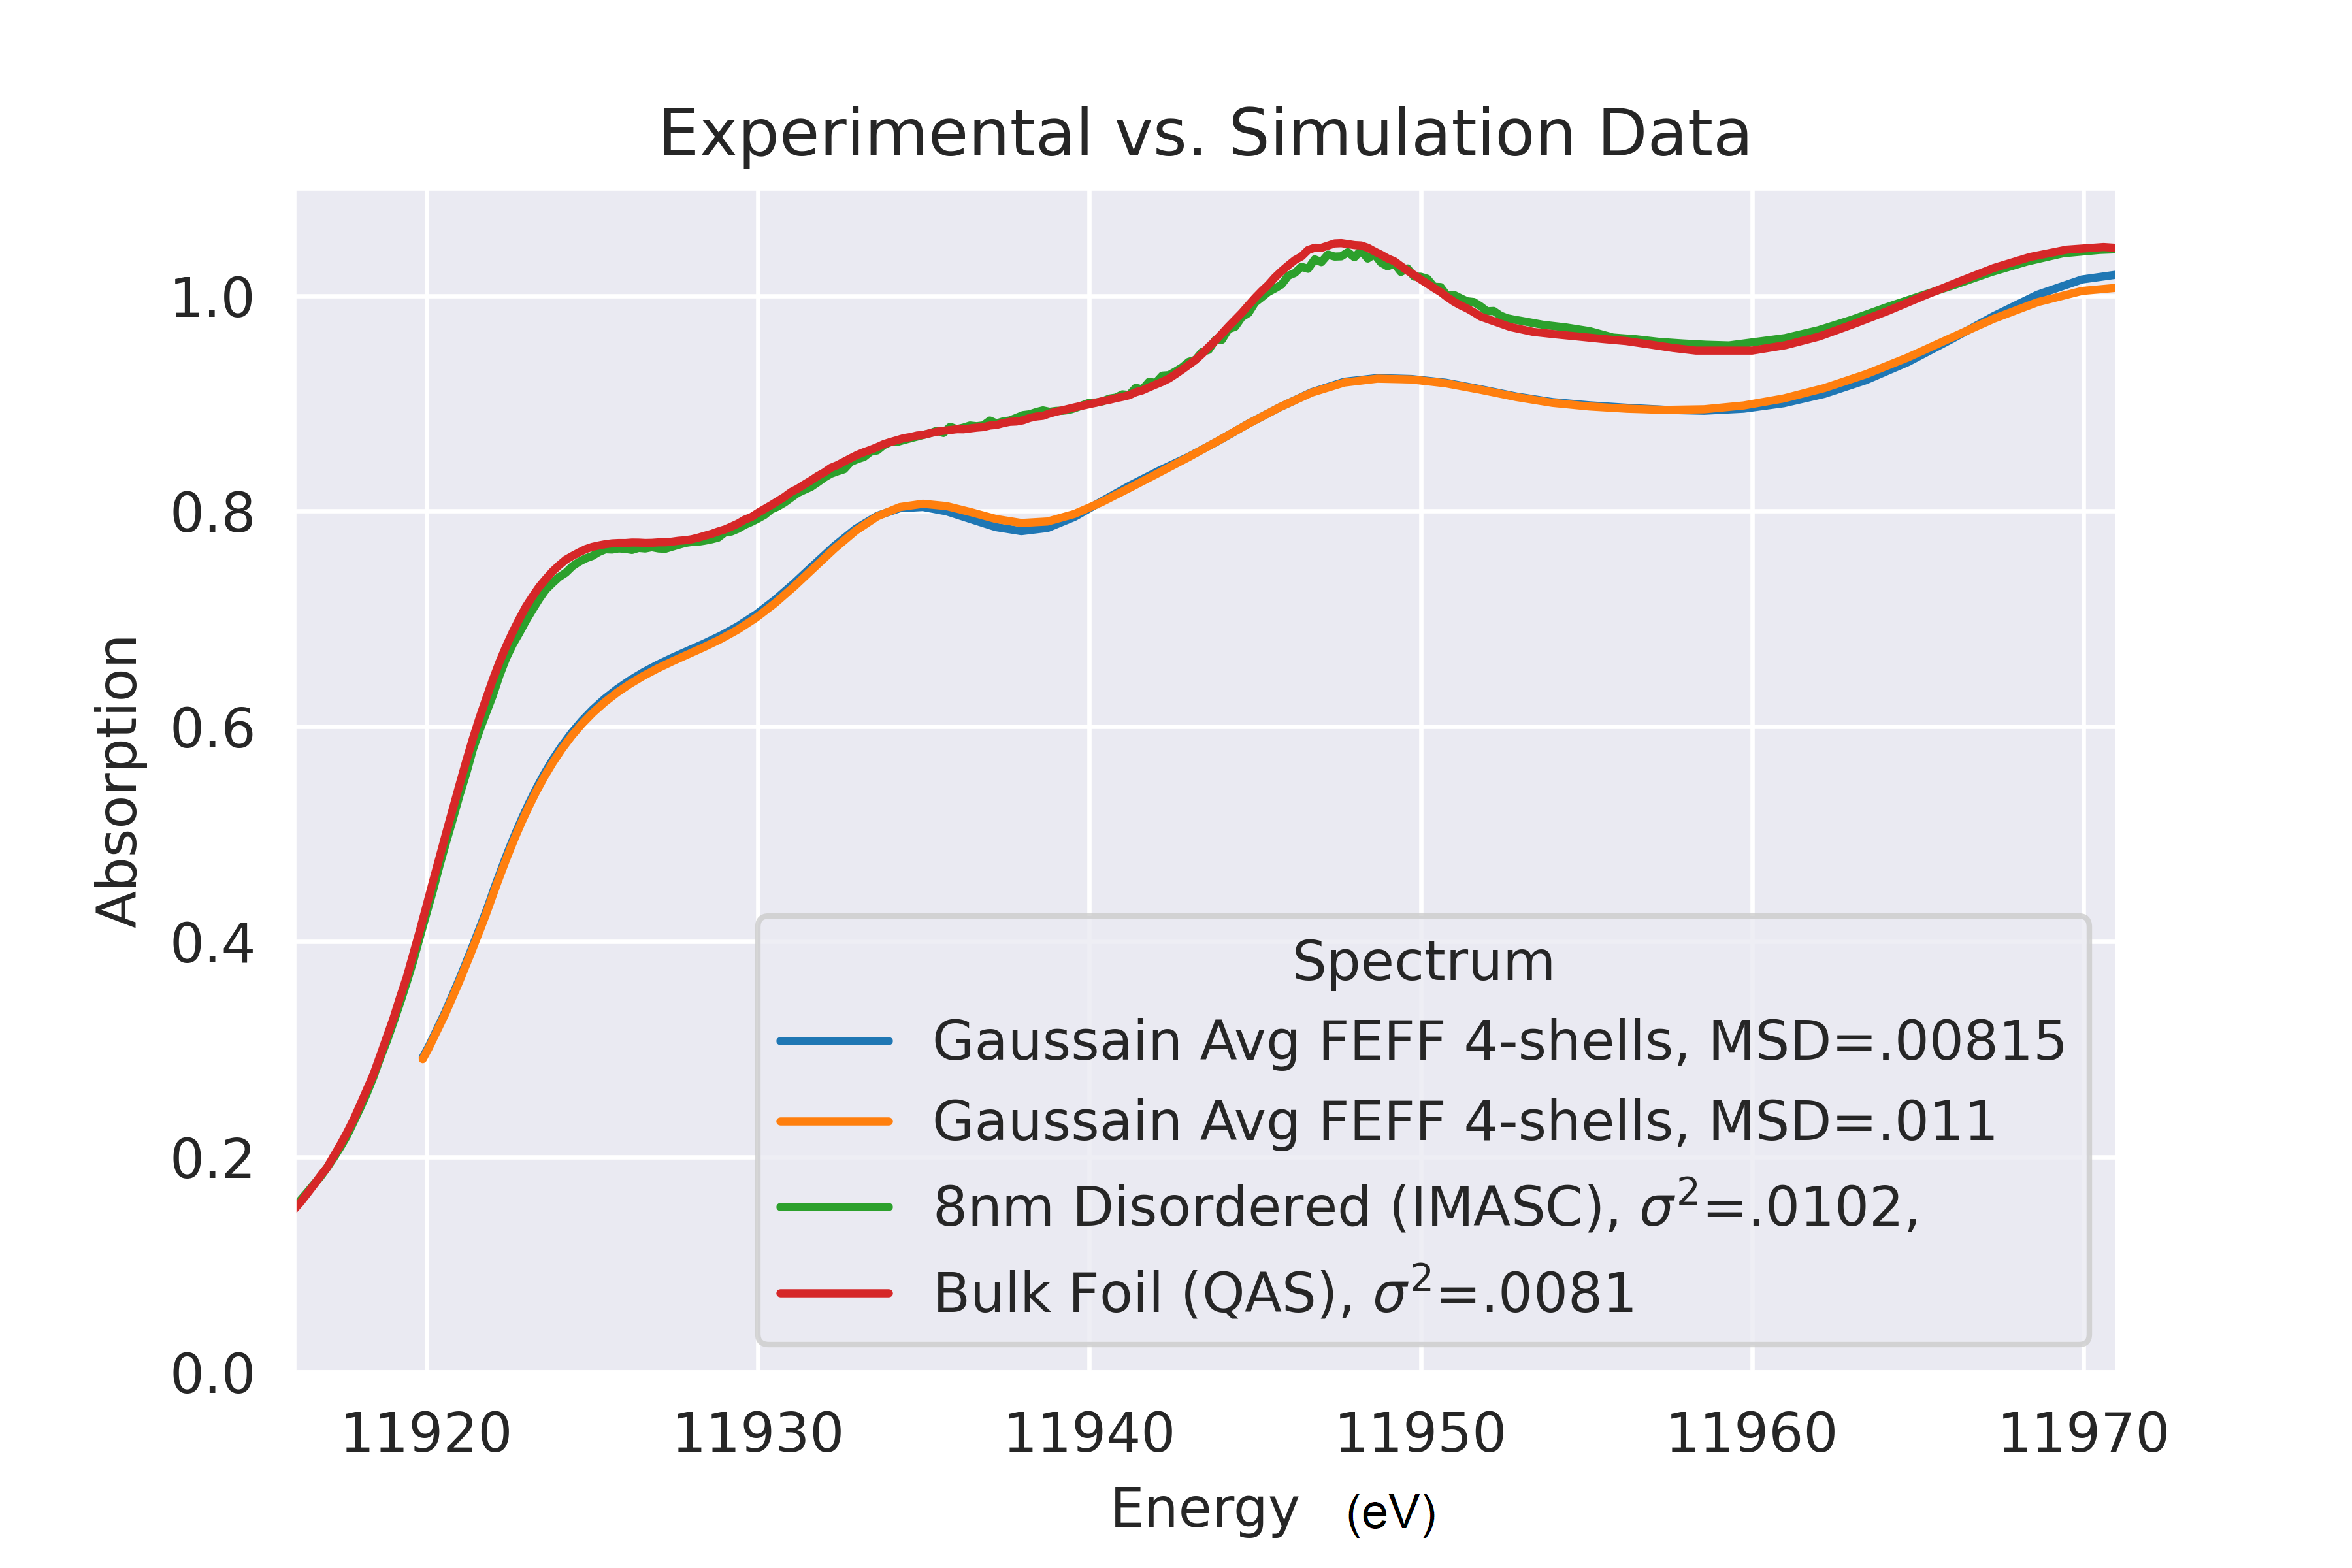
\includegraphics[width=.75\linewidth]{Chapters/Figures/updated_bulk_8nm_disorder_experimental_theory_comparison.png}
	\caption[Simulation vs. Experimental]{Comparing the bulk foil (red) measurement to the 8~nm disordered nanoparticle (green) measurement is an analog to comparing the simulated, non disordered FEFF spectrum (blue) to the simulated disordered spectrum (orange).}
	\label{fig:avg-experimental-vs-simulation}
\end{figure}

In Figure \ref{fig:avg-experimental-vs-simulation}, the bulk Au foil spectrum is above the 8~nm nanoparticle spectrum (more absorption) until the peak around 11937~eV, where the NP absorption becomes higher. The two criss-cross again over the next two peaks, changing which material has the higher absorbance in an energy range. This change is more easily seen in Figure \ref{fig:avg-experimential-vs-simulation-difference}, which plots the difference between the the bulk material and the nanoparticle absorption for both the experimental measurements and the simulations. The experimental and simulation difference-spectra follow the same trend with the exception of the peak around 11947~eV.
% The two spectrum switch again at the peak around 11943~eV so the bulk foil's absorption nlevel is higher again. Beyond this peak, the two


\begin{figure}[h!]
	\centering
	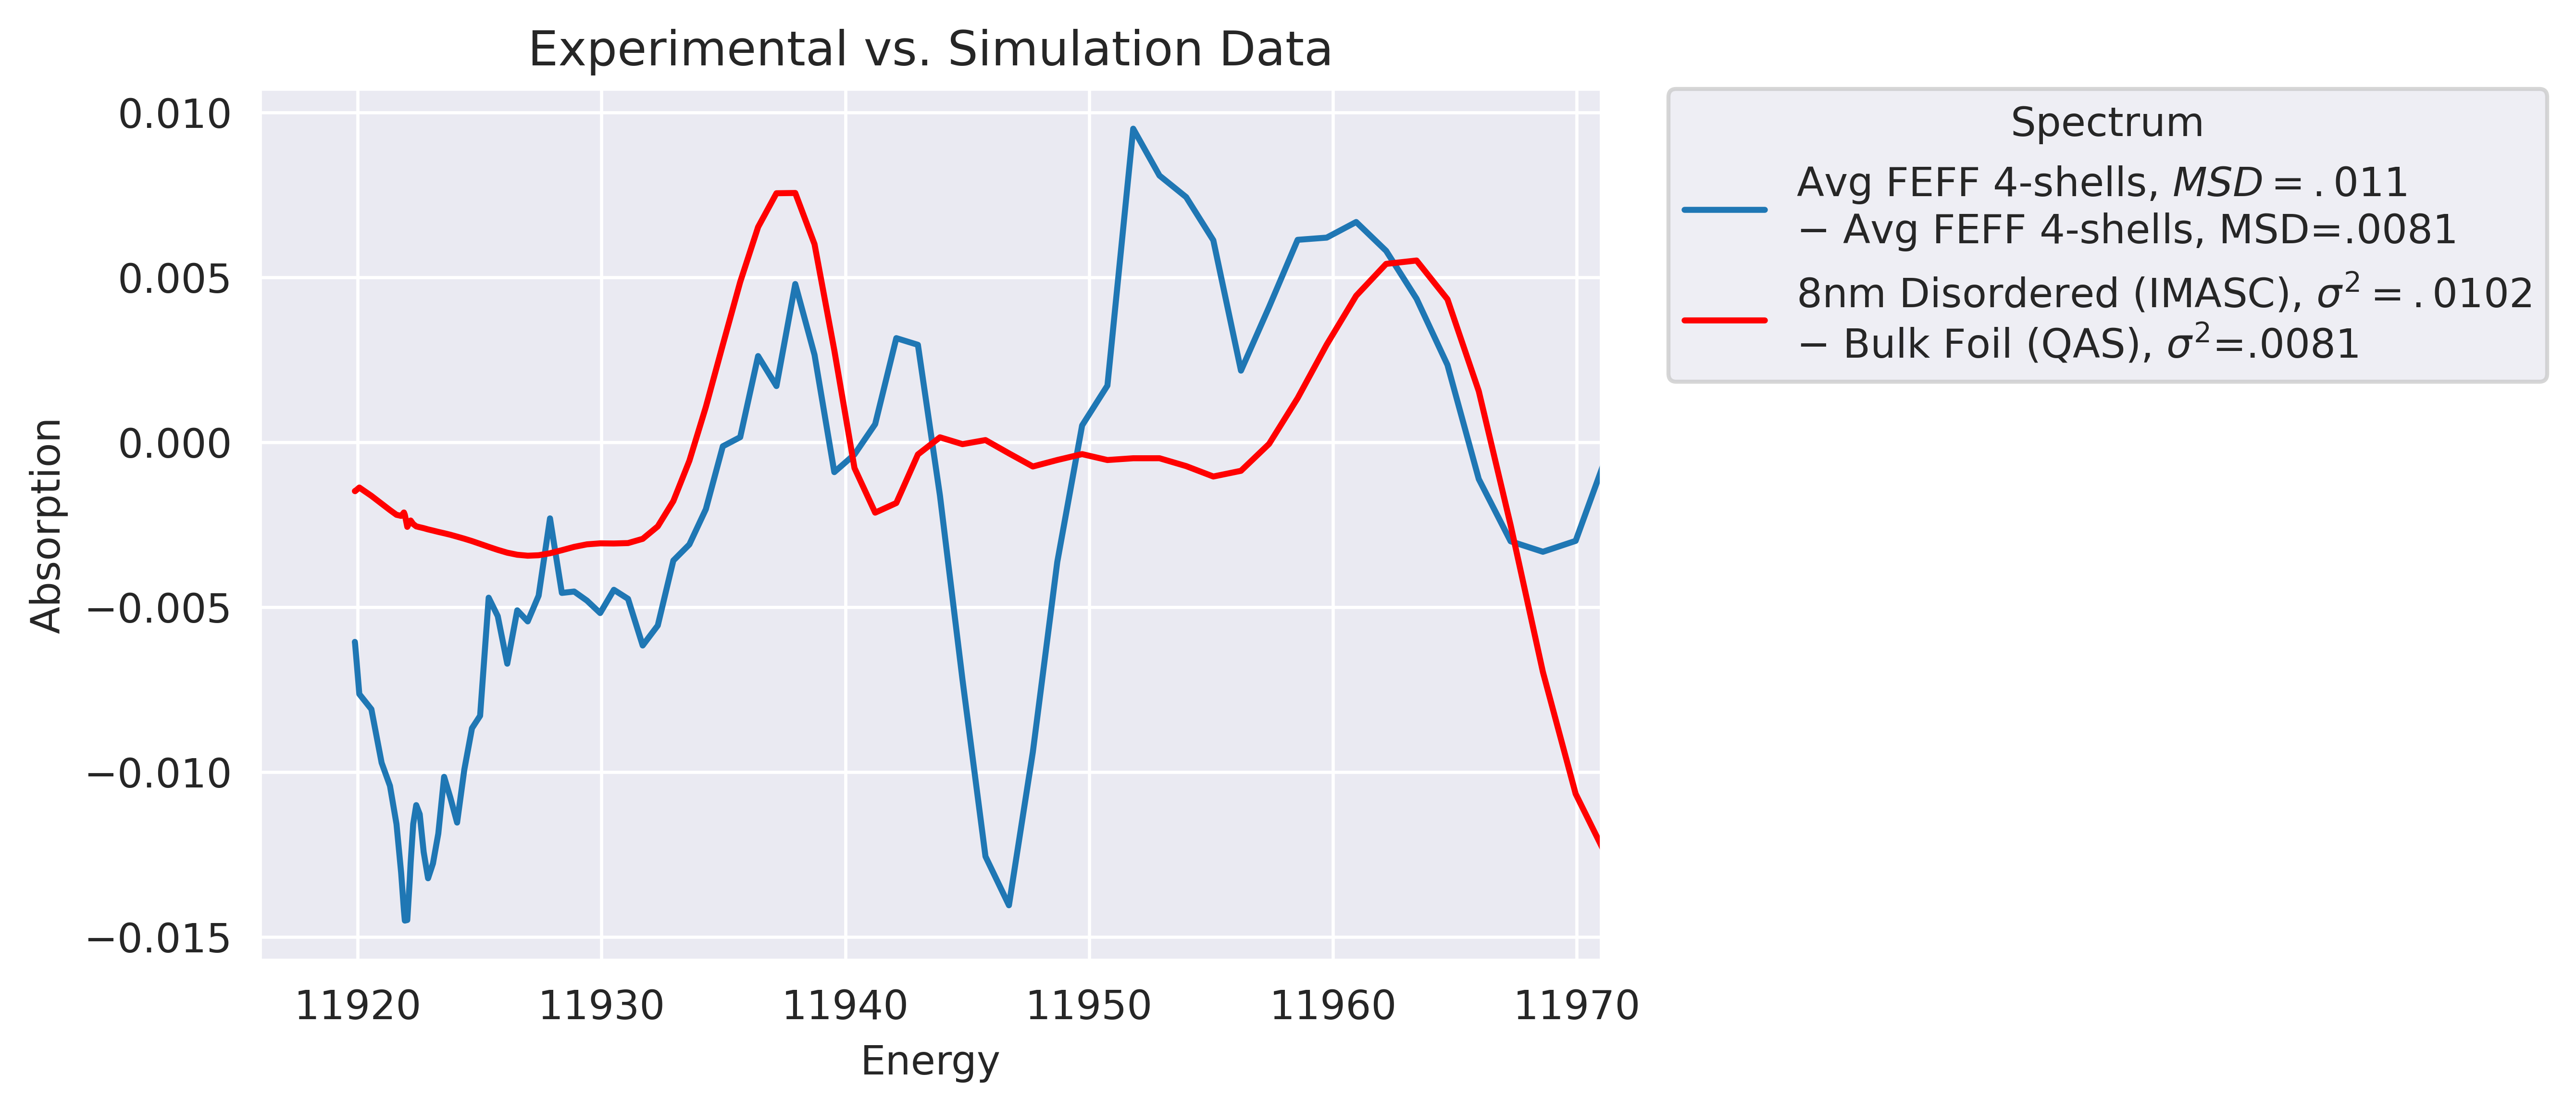
\includegraphics[width=\linewidth]{Chapters/Figures/experimental_vs_simulation_delta.png}
	\caption[Bulk-nanoparticle difference: Simulation vs. Experimental data]{The difference between the nanoparticle spectrum and the bulk spectrum are plotted for the same data as in Figure \ref{fig:avg-experimental-vs-simulation}. It is easier to see where the bulk and the nanoparticle absorption crisscross by plotting the difference.}
	\label{fig:avg-experimential-vs-simulation-difference}
\end{figure}

Figures \ref{fig:avg-experimental-vs-simulation} and \ref{fig:avg-experimential-vs-simulation-difference} aren't meant to be perfect comparisons of simulations vs. experimental data. For one, the experimental data compares a bulk spectrum to a nanoparticle. By contrast, both the simulation spectra are of the same size 55 atom cluster. Still, much of the disorder trends are coded in the simulation approach. 

To test if the size information is also coded in our simulations, we compare different size simulations to experimental data in Figure \ref{fig:avg-experimental-vs-simulation2}. As expected, including more atoms in the simulation produces more bulk-like spectrum characteristics, such as larger amplitude peaks.

\begin{figure}[h]
	\centering
	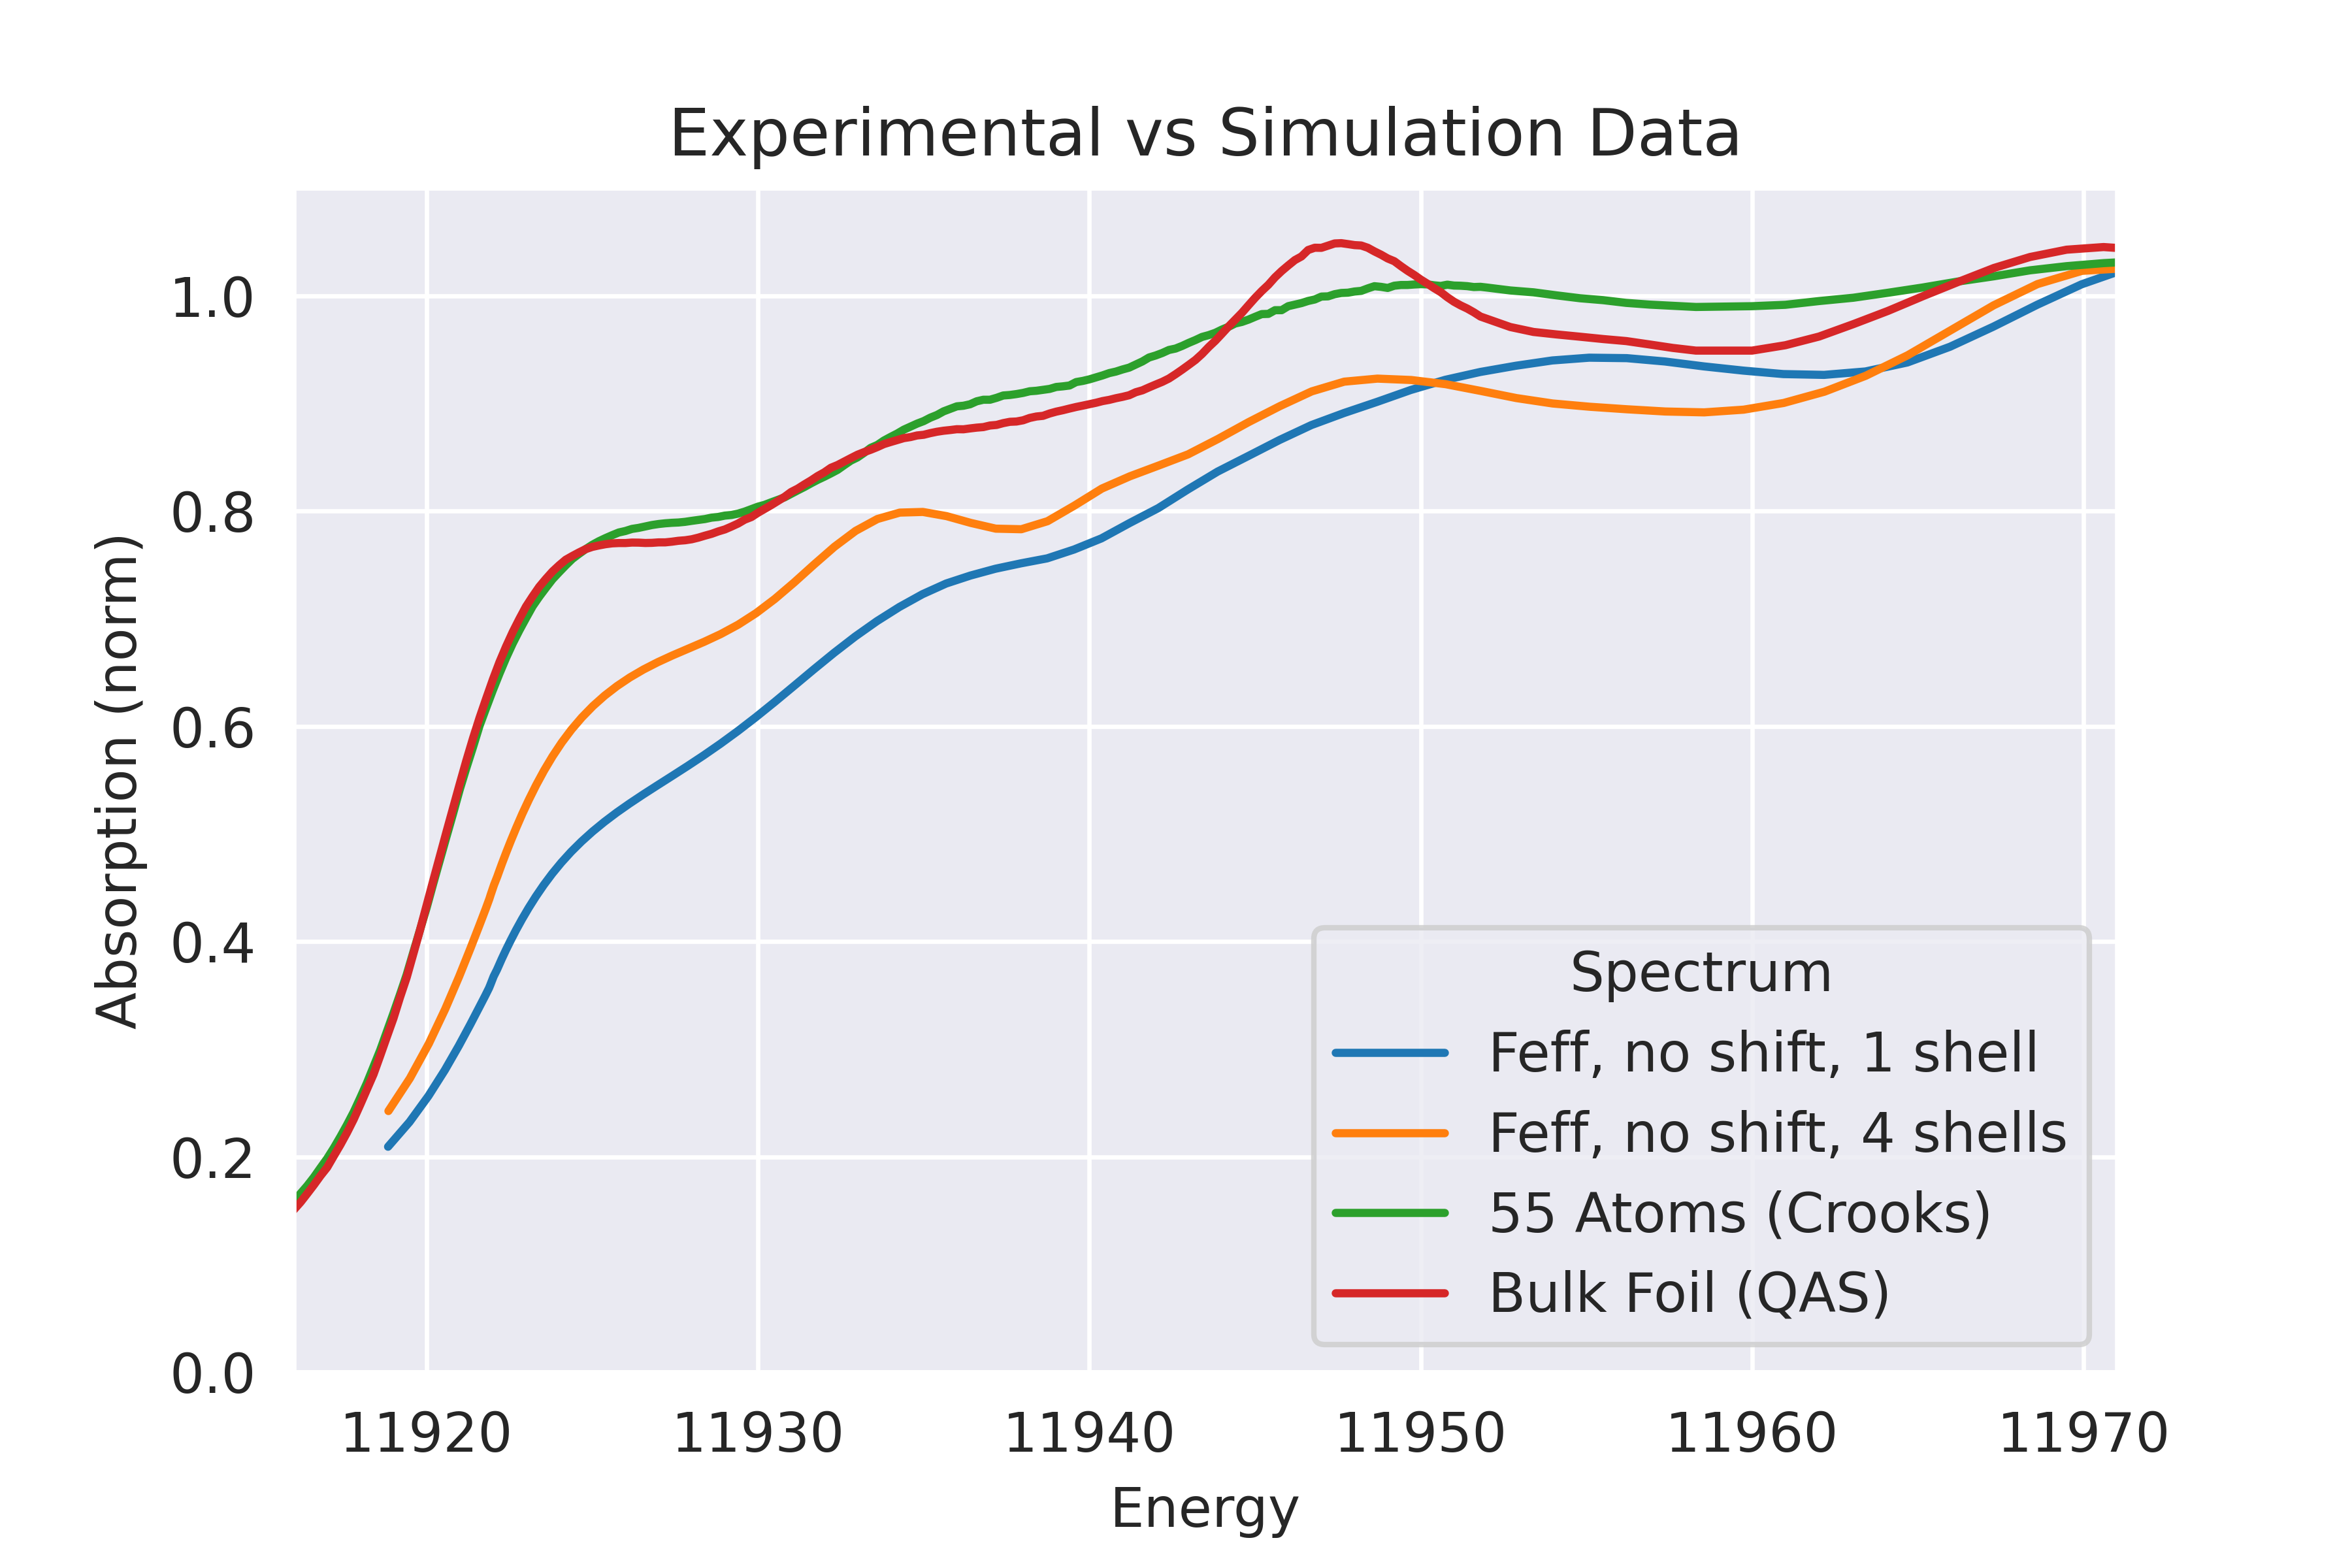
\includegraphics[width=.7\linewidth]{Chapters/Figures/Bulk_55atom_experimental_theory_comparison.png}
	\caption[Simulation vs. Experimental 2]{Comparing the bulk foil (red) measurement to the 55 atom nanoparticle (green) measurement is an analog to comparing the 13 atom simulated spectrum (blue) to the 55 atom simulated spectrum (orange).}
	\label{fig:avg-experimental-vs-simulation2}
\end{figure}

I NEED A PLOT COMPARING THIS METHOD TO PARTICLE AVERAGED METHOD HERE.

\section{Particle-Averaged FEFF Simulated Disordered Structures} \label{sec:pa-feff-vs-gaussian-feff}

\begin{figure}[h]
	\centering
	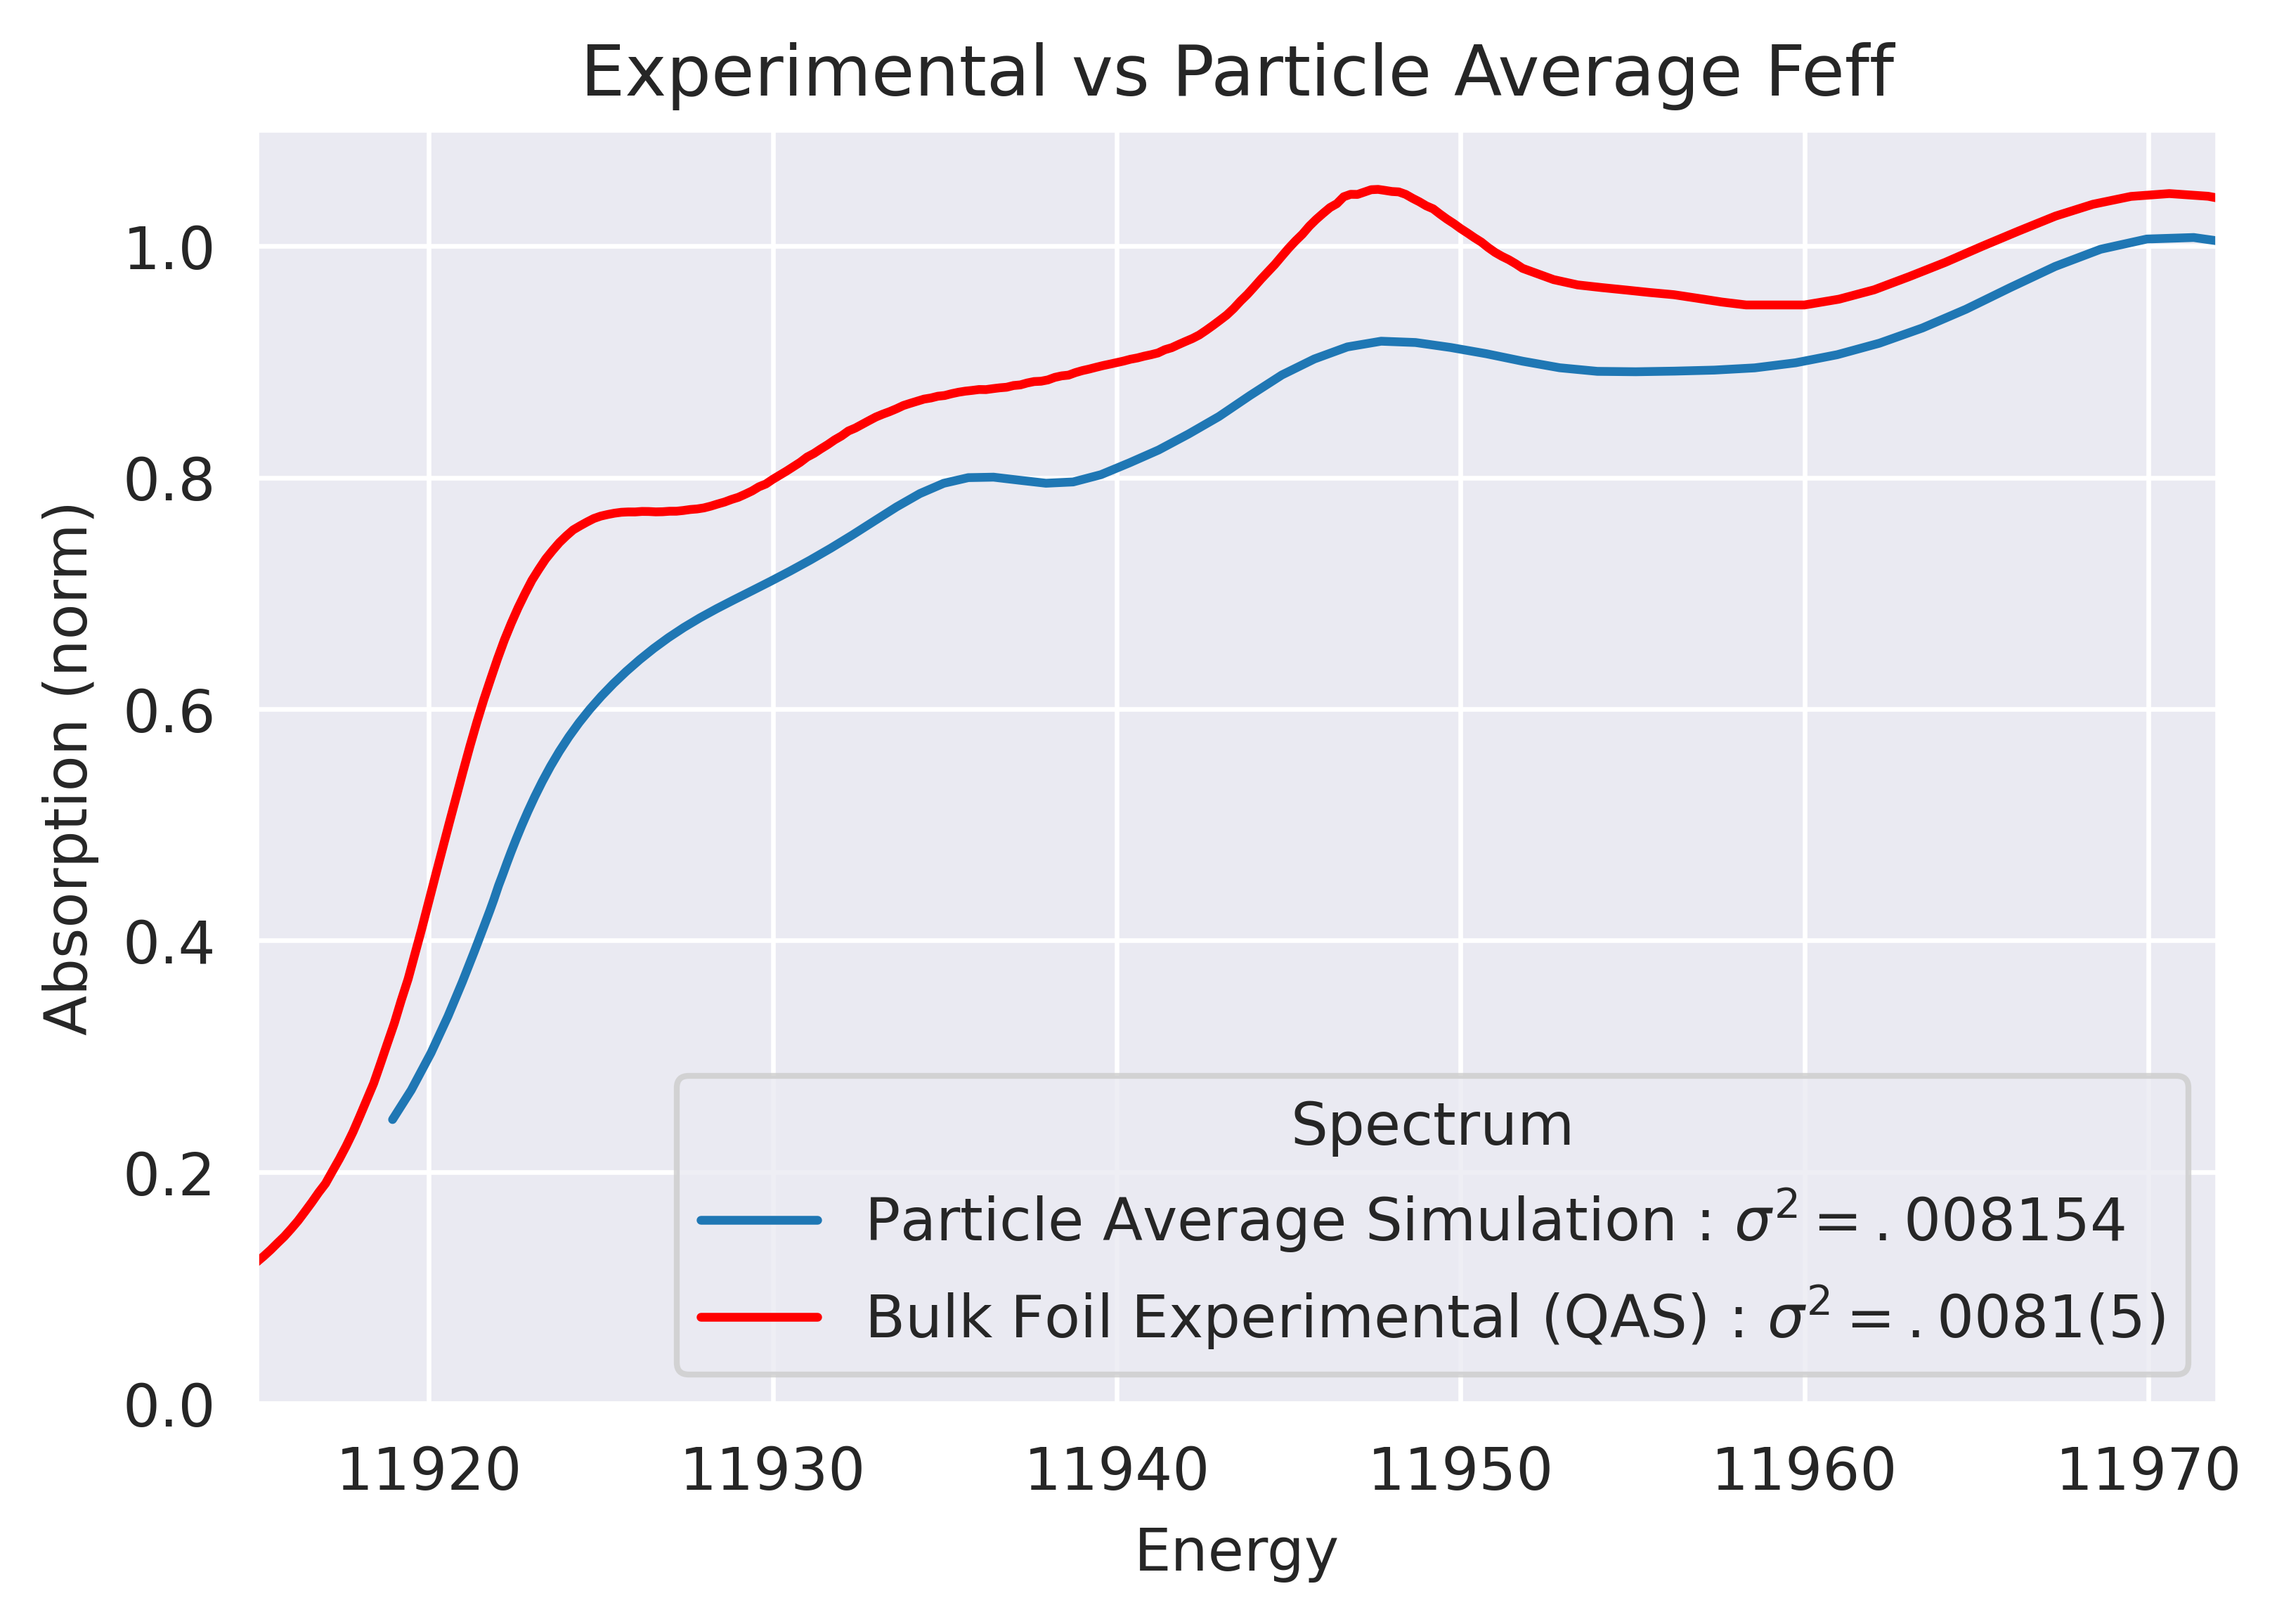
\includegraphics[width=.7\linewidth]{Chapters/Figures/Bulk_experimental_vs_pa_comparison.png}
	\caption[Simulation vs. Experimental 3]{Comparing the bulk foil (red) measurement to a simulated large, bulk-like nanoparticle with the same disorder. The FEFF-}
	\label{fig:avg-experimental-vs-simulation2}
\end{figure}

\section{Traditional Particle-Averaged Simulations} 
\label{sec:traditional-disorder}


\chapter{Machine Learning}
%Chapter 3
Predicting disorder from XANES spectra requires a sophisticated model or algorithm capable of extracting non-linear features from the data. Increasing the disorder in the structure does not simply shift or scale the spectrum by a scalar; instead, disorder alters the spectrum in a complex and unknown way, for which we rely on machine learning  (ML) to discern. The general goal of ML is to recognize patterns in data, iteratively learning to solve complex, non-linear problems to make powerful predictions on new, unseen data \cite{ML-and-the-physical-sci}. Due to the integral role ML plays in this thesis, the following chapter serves to establish how neural networks fundamentally work. All terms necessary for understanding the specific neural network implementation discussed in the chapter \ref{ch:results} will be defined here.

First, we clarify the distinction between the following commonly misused terms: machine learning (ML), deep learning, and artificial intelligence (AI). ML refers to the general computational technique of fitting a model to a collection of data utilizing an iterative training process. These models can either be regressors or classifiers, the former predicts a continuous range of values, and the latter being a discrete predictor. Neural networks are one example of a machine learning model that tends to be computationally intensive. They are capable of creating highly non-linear models able to solve complex tasks such as object detection \cite{szegedy2013deep} or speech recognition \cite{ms-speech-recognition-paper} \cite{speech-recognition}. Neural networks were inspired by biological nervous systems; consequently, graphical representations of ANNs include common terms such as ``nodes'' and ``connections.'' The field of ML involving ANNs with many layers is referred to as deep learning \cite{schmidhuber2015deep}. AI is a subfield of deep learning where a neural network is trained to generate human-like responses. Common examples of AI are generative chatbots \cite{chatbots} and a virtual assistants \cite{virtual-assistants} \cite{virtual-assistants2}. 

With these definitions, to predict disorder from XANES we utilize deep learning to train a regression-based neural network. The following sections will walk through the mathematical process of training a simple neural network. In practice, sophisticated APIs such as Google's TensorFlow \cite{tensorflow2015-whitepaper} or Facebook's PyTorch \cite{pytorch-paper} handle the mathematical backend and optimization; however, one must first build a fundamental understanding of the methods these frameworks are executing before attempting to implement them.
% \cite{tensorflow2015-whitepaper} 
% \cite{pytorch-paper}
\section{Feedforward and Backpropagation in ANNs}

Understanding how a neural network makes a prediction requires a solid grasp of linear algebra. The process where a NN passes information from the input to the subsequent layers to make a prediction is called the feedforward process. The name comes from the operation where each layer of the NN passes information to the next layer until the reaching output layer. The process of updating the weights of the NN is called backpropagation and relies principally on vector calculus. Neither action is particularly mathematically complicated; however, there are so many parts that it is easy to get lost in the sea of similar-sounding partial derivatives. In this next section, we explicitly walk through the math for the feedforward process of a fully connected (affine) neural network.

\subsection{Feedforward}
Consider the neural network in figure \ref{fig:simpleNN} with an input layer of three nodes, a single hidden layer with five nodes, and an output layer with two nodes. The input layer (zeroth layer) has a cardinality of $ \mu=3 $ and is represented in Einstein notation\footnote{Recall that in Einstein notation repeated indices are implicitly summed over.} as a row vector $ x_\mu $. Each edge in the graph represents a weight that is multiplied with the connected node on the left. Each node in the input layer is multiplied by the weight of the connected edge and added together. This operation for all input nodes and weights can thus be represented as a dot product between the input layer row vector and a weight matrix. The hidden layer (first layer) has a cardinality of $ \nu=5 $. Thus, the resulting dot product is $ x_\mu W_\nu^{\mu(1)} $ where $ W_\nu^{\mu(1)} $ represents the matrix of weights to create the first layer. While this result has the correct dimensionality for the hidden layer, there are still two operations reuired to produce the actual values for the nodes $ h_\nu^{(1)} $. First, a small trainable parameter, $ b_\nu $  is added to every value from the previous calculation. The values in this row vector are called biases and are introduced to prevent overfitting---i.e. the phenomenon where a model predicts the training data well, but is unable to generalize and predict un-seen data. Biases are a regularization parameter. Regularization techniques are discussed below. An example is provided in Figure \ref{fig:overfitting}. The final operation applied to produce the first hidden layer's values is known as an activation function. Without an activation function, a neural network would be unable to learn non-linear features. There are several types of activation functions, the three most common being sigmoid, tanh, and ReLu.


\subsubsection{Sigmoid and Tanh}
The sigmoid activation function is defined as the following:
\begin{equation}
    \label{sigmoid}
    \sigma (x) = \frac{1}{1 + e^{-x}}
\end{equation}

The sigmoid activation function maps the input between zero and one. Hence, sigmoid activation functions are often used in the final layer to output a probability. The sigmoid function approaches 1 and -1 around $ x=4 $ and $ x=-4 $ respectively, meaning that the sigmoid activation function is only useful within that limited range. One issue with both these activation functions is the potential for creating a vanishing gradient. The gradient of either of these functions approaches zero for values above four. This asymptotic approach hurts the ability of the NN to meaningfully update its trainable parameters. The importance of calculating the gradients of these activation functions will be discussed in the next section in the context of backpropagation. 

\begin{figure}[h!]
    \centering
    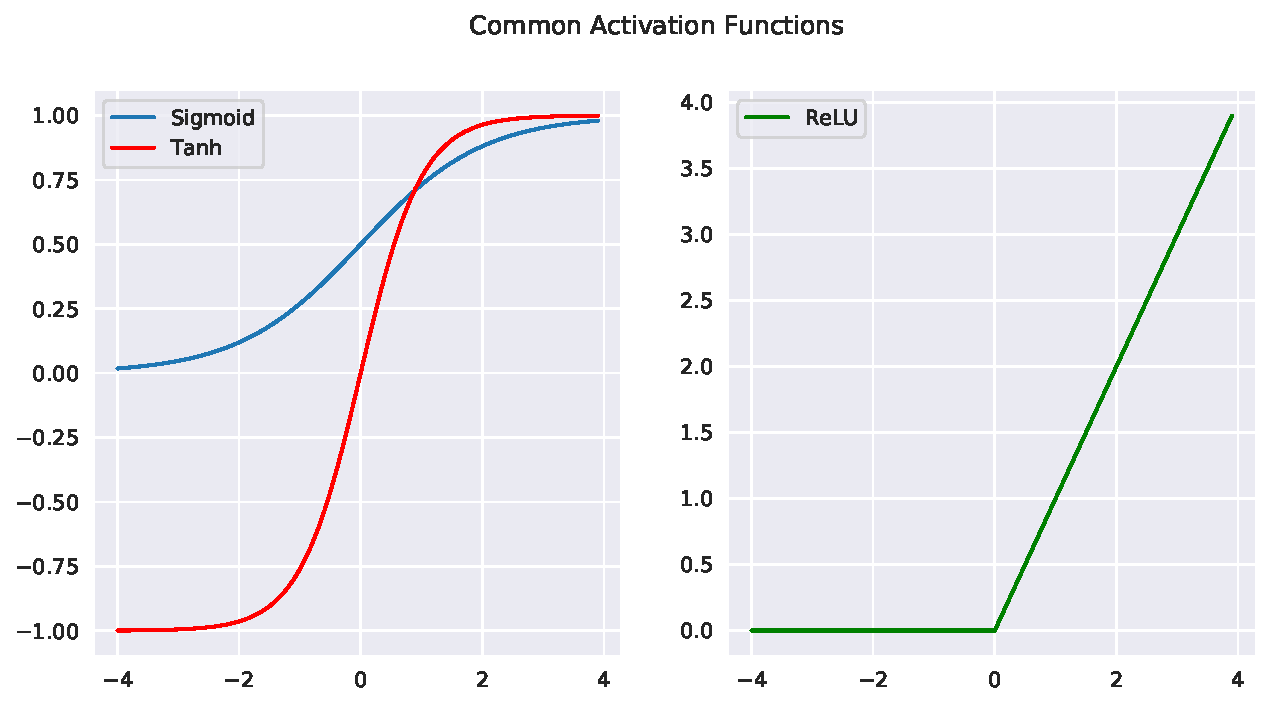
\includegraphics[width=\linewidth]{Chapters/Figures/sigmoids2.pdf}
    \caption[Activation-Functions]{Plotted above are three common activation functions: sigmoid, tanh, and ReLU. Simgoid and tanh are particularly useful for scaling the output of a neural network layer to be within a given range. ReLU and its variations are useful for deep ANNs, where vanishing gradients are problematic.}
    \label{fig:ActivationFunctions}
\end{figure}

\subsubsection{ReLU}
The \textbf{Re}ctified \textbf{L}inear \textbf{U}nit activation function, or ReLU has become an important staple of machine learning. The activation function, $ f(x) $, is defined as the following:
\begin{equation}
f(x)=
\begin{cases}
    0 & \text{if } x <= 0 \\
    x & \text{if } x > 0
\end{cases}
\end{equation}

\noindent ReLU is important because it provides a much greater range in values. Whereas the sigmoid and tanh activation functions saturate around 4, ReLU never saturates for linear values. Additionally, ReLU is simple to calculate and tends to help neural networks converge quickly. Arguably thier most major benefit is the reduced likelihood of creating a vanishing gradient. Further, because ReLU returns 0 for any negative value fed foward into the node, many ReLU activation functions in a given layer help lead to sparser layers, reducing the overall complexity of the model and helping prevent overfitting.


\begin{figure}[h]
    \centering
    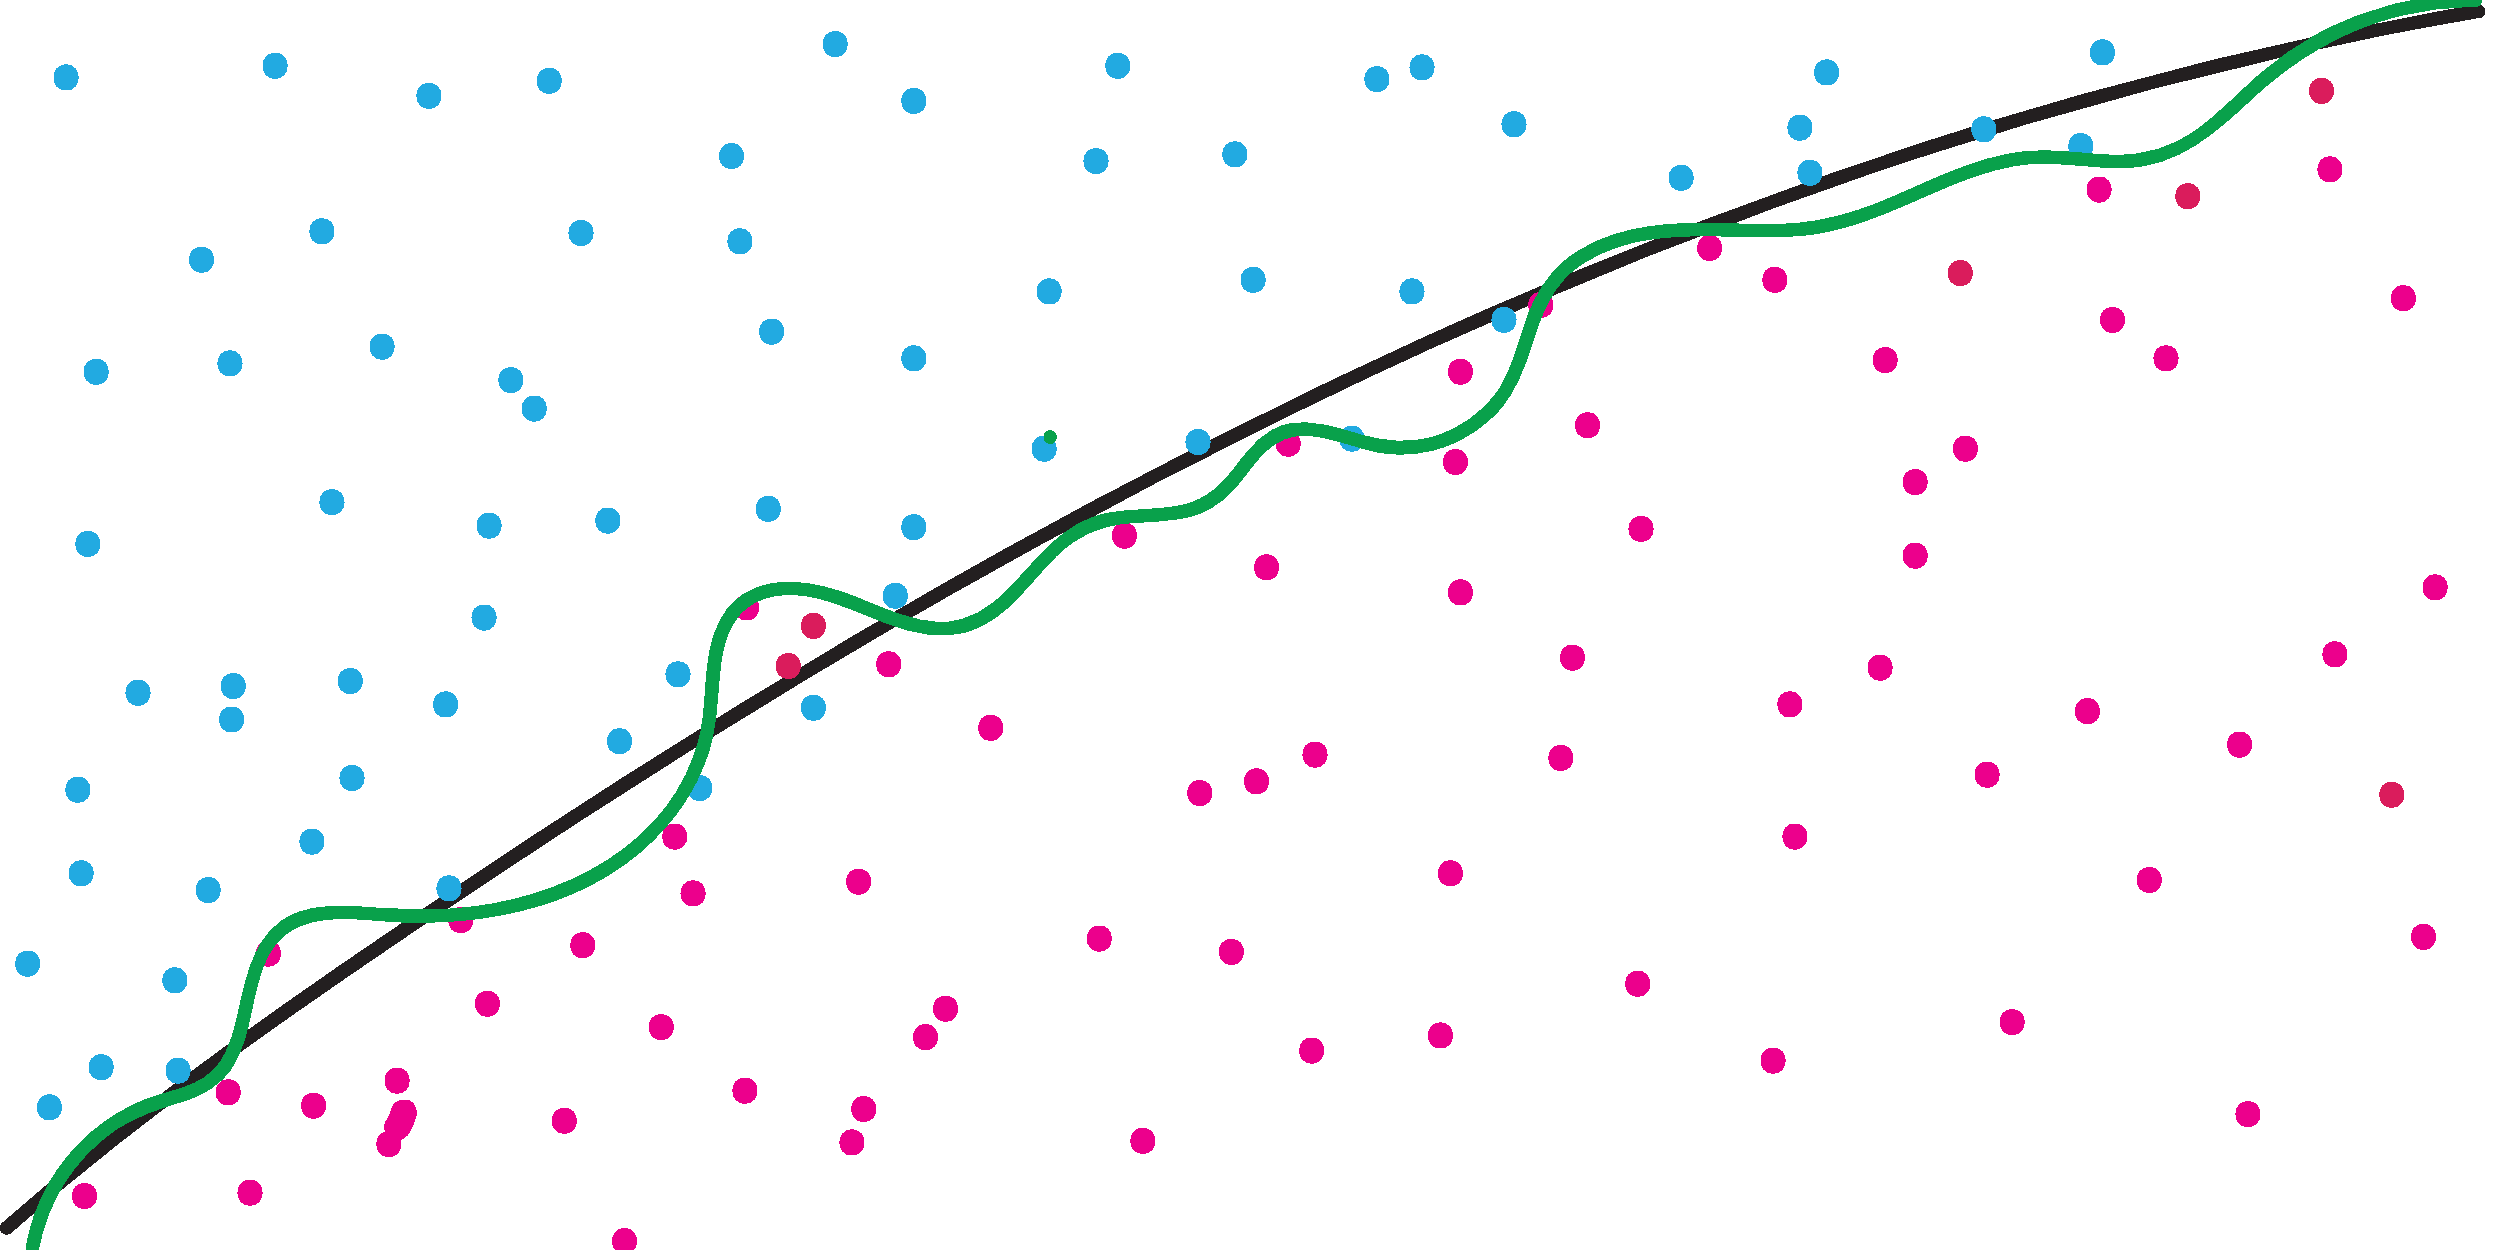
\includegraphics[width=\linewidth]{Chapters/Figures/overfittingOrig2.pdf}
    \caption[Overfitting]{The green curve represents a model overfitting a binary classification problem. Although it makes near-perfect predictions for the training data in this figure, the model will not generalize as well as the simpler black curve when it tries to predict new, unseen data. Introducing biases and dropout layers in neural networks are strategies to prevent overfitting to reduce the model variance and fit the data like the black curve.}
    \label{fig:overfitting}
\end{figure}


With the input nodes dotted with the weights, the baises added, and then the activation function calcuated for each node, we arrive at the final final for the first hidden layer. Mathematically, $ h_\nu^{(1)} = \sigma\left( x_\mu W_\nu ^\mu + b_\nu \right) $. This process is now repeated, only with the starting layer $ h_\nu^{(1)} $ and the output
$ \hat{y} = \sigma \left( h_\nu W_\kappa ^\nu + b_\kappa \right)$ is the final output of the neural network. The equations for each step as well as the dimensionality of each layer can be found in Figure \ref{fig:simpleNN}.

\begin{figure}[h!]
    \centering
    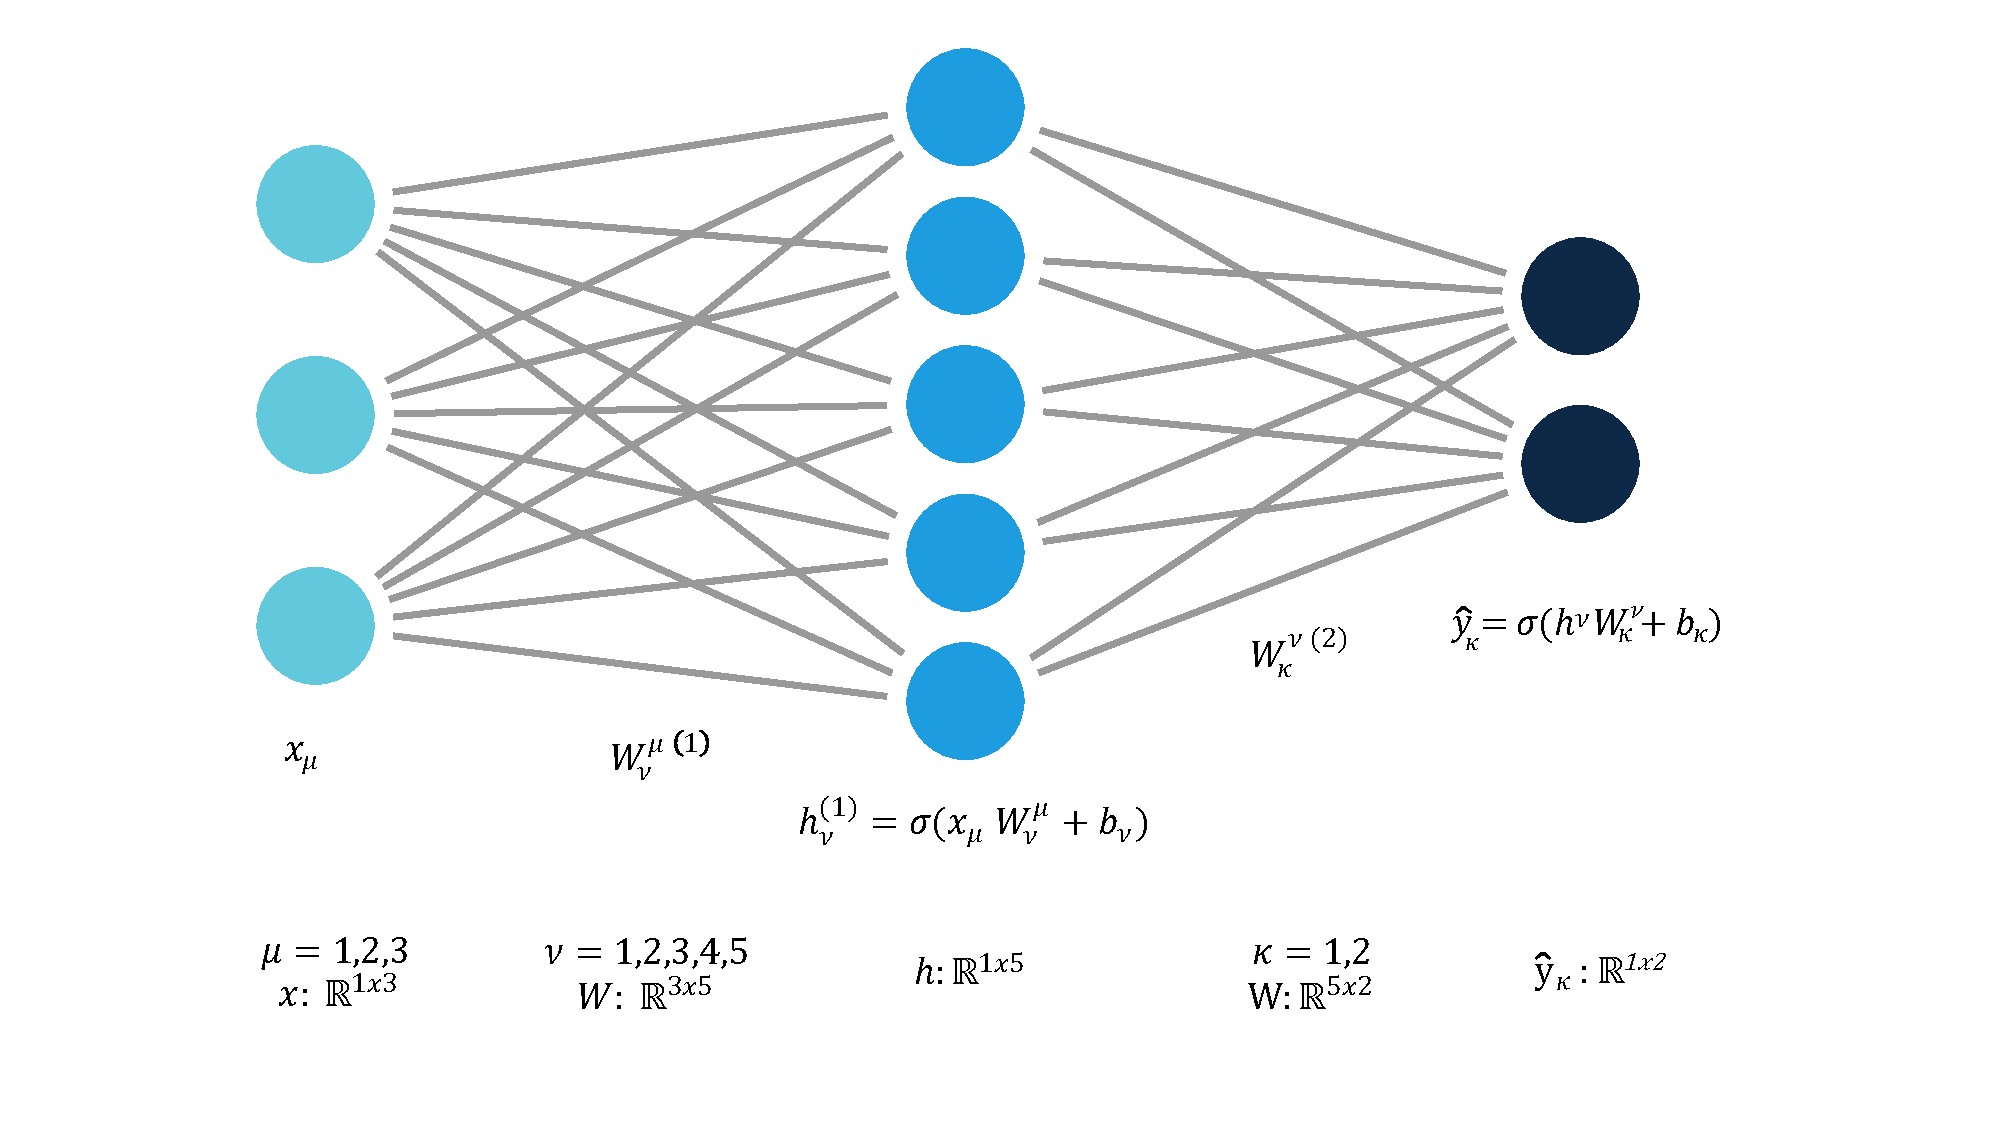
\includegraphics[width=\linewidth]{Chapters/Figures/einstein_NN_2.pdf}
    \caption[Neural Network Example]{This diagram of a fully connected (affine) neural network has a single hidden layer and two output nodes. The tensors for each hidden layer are written in Einstein notation. The implicitely summed over greek letters and dimensionality are written below the tensors for clarification.}
    \label{fig:simpleNN}
\end{figure}

\subsection{Loss Metrics and Regularization}
In order to update the netork parameters, it is necessary to evaluate the quality of every prediction the neural network makes. The measure of the error in one prediction is referred to as the \textit{loss}, and the summed total of all the errors in predictions is called the \textit{cost}. For regression problems, the two most common cost functions are the mean squared error and the mean absolute error \cite{regularization-2017survey}. These are also referred to as the L2 and L1 costs, respectively, and defined as:

% \begin{align}
%     \label{eqn:lossFunctions}
%     \text{L1 Cost} &= \frac{1}{n} \sum_i \abs*{\hat{y_i} - y_i} \\
%     \text{L2 Cost} &= \frac{1}{n} \sum_i \left( \hat{y_i} - y_i \right)^2
% \end{align}
\begin{align}
    \label{eqn:lossFunctions}
    \text{L1 Cost} &= J = \sum (\hat{y}_i - y)^2 + \lambda \sum \abs*{W} \\
    \text{L2 Cost} &= J = \sum (\hat{y}_i - y)^2 + \lambda \sum (W)^2
\end{align}

\noindent where $ n $ is the number of training sampels. The equation for updating the weights under L2 regularization is as follows:
\begin{equation}
    W := (1-\alpha \lambda)W - \frac{\partial J}{\partial W}  
\end{equation}

\noindent where $\alpha$ is the learning rate, $\lambda$ is the regularization hyper-parameter, and J is the cost. L2 regularization is often referred to as weight decay. Every iteration the weights are pushed closer to zero due to the multiplicatiion of the weights by a value $<1$. L1 is known as LASSO (least absolute shrinkage and selection operator), because it shrinks the less important features' coefficients to zero. This is because for small values $\abs*{w}$ is a much stiffer penalty than $w^2$. Thus, L1 is thus a good choice when you have a dozens of features.

% \noindent Explicitly, for one component of the hidden layer:

% \begin{align}
%     h_j &= \sigma(w_{1j}x_1 + w_{2j}x_2 + w_{3j}x_3 + w_{4j}x_4 + w_{5j}x_5 + b_j) \\
%         &= \sigma\Big(\sum_{i=1}^{i=5}w_{ij}x_{i} + b_j\Big)
% \end{align}

Dropout layers are another variation of model regularization used exclusively for neural networks \cite{dropout-srivastava2014}. The idea is to introduce a hidden layer with a probability ``dropping out,`` i.e. ignored. Large weights in a neural network are indicative of a high-variance network, likely to be overfitting the data. By indroducing layers with a probability of dropping out, the inward connection to the next layer change stochastically from batch to batch. This has the effect the adding noise to the network, similar to the inclusion of biases \cite{conv-dropout-layers} \cite{conv-dropout-layers2}.

\subsection{Backpropagation}
Backpropagation is the process of updating all the trainable parameters of the machine learning model, including weights, biases, and any other trainable parameters. The partial derivative require repeated use of the chain rule. Representing the above neural network as a functional yields the equation:

% \begin{equation}
%     \hat{y} = \sigma\left( g \left( f() \right) \right)
% \end{equation}
% \noindent This would be a network with inputs $(x, y)$, two hidden layers ($ f $  and $ g $ ), and an output with activation function sigma. Let's say the loss is the RMS loss. Thus,

\begin{equation}
    \label{eqn:functional}
    \hat{y} = \sigma \left( h_\nu ^{(1)} \left( x_\nu \right) \right)
\end{equation}

\noindent where the the output layer $ \hat{y} $ is a function of the hidden layer, $ h_\nu ^{(1)} $ which in turn is a function of the input layer $ x_\mu $. Consider the L2 loss (\ref{eqn:lossFunctions}). Note that the loss function is a function of the previous functional (\ref{eqn:functional}). To see how much to shift the weights, calcuate the gradients for each layer. The first partial derivative is trivial:

\begin{equation}
    \frac{\partial J}{\partial J} = 1
\end{equation}

\noindent For the next layer (the output layer):

\begin{equation}
\frac{\partial \hat{y}}{\partial J} = \frac{\partial J}{\partial J}\frac{\partial \hat{y}}{\partial J}
\end{equation}


\noindent For the next nested-function (the sigmoid):

\begin{equation}
\frac{\partial J}{\partial \sigma} = \frac{\partial J}{\partial \hat{y}} \frac{\partial \hat{y}}{\partial \sigma}
\end{equation}


\noindent The next layer is the hidden layer before the activation function. For simplicity it will be referred to as $ g $ where $ g = x_\mu W_\nu ^\mu + b_\nu $.  

\begin{equation}
    \frac{\partial J}{\partial g} = \frac{\partial J}{\partial \hat{y}} \frac{\partial \hat{y}}{\partial \sigma} \frac{\partial \sigma}{\partial g}
\end{equation}


\noindent Next layer is the input layer, $ X_\mu $ has no trainable parameters, so the process for this network architecture is complete. If there were more hidden layers, the chaining rule would continue by multiplying the gradient calculated in the previous step by the gradient of the next layer with respect to the previous layer (towards the input layer). 

% \begin{equation}
%     \frac{\partial L}{\partial f} = \frac{\partial L}{\partial \hat{y}} \frac{\partial \hat{y}}{\partial \sigma} \frac{\partial \sigma}{\partial g} \frac{\partial g}{\partial f}
% \end{equation}

\subsection{Concrete Example}

Finally, we will repeat the backpropogation process of updating the weights for the previous example as explicitly as possible. Consider again the functional $ \hat{y} $ in equation (\ref{eqn:functional}) and the L2 loss in equation (\ref{eqn:lossFunctions}), rewritten here as $ L $ . To determine how do shift the weights in the function, want to know $\frac{\partial J}{\partial W}$, where $ W  $ is short for $ W_\kappa ^{\nu (2)} $, the weight matrix connected to the second layer (the output layer). 

\begin{align}
L = \frac{1}{m}\sum(\hat{y} - y)^2 \\
\end{align}

\noindent As before, the first partial derivative is trivial

\begin{equation}
    \frac{\partial J}{\partial J} = 1
\end{equation}

\noindent and the next partial derivative is also strait-foward:

\begin{equation}
\frac{\partial J}{\partial \hat{y}} = 2(\hat{y} - y )
\end{equation}

\noindent Applying the chain rule yields:

\begin{equation}
\label{eqn:dldy}
\frac{\partial J}{\partial \hat{y}} = \frac{\partial J}{\partial J}\frac{\partial J}{\partial \hat{y}} \\
= 1 \cdot 2(\hat{y} - y )
\end{equation}

\noindent The next required term in the chain is the derivative of the loss with respect to the sigmoid:

\begin{equation}
\frac{\partial J}{\partial \sigma} = \frac{\partial J}{\partial \hat{y}} \frac{\partial \hat{y}}{\partial \sigma}
\end{equation}

\noindent We already found the first term (\ref{eqn:dldy}), and the second term in trivial.

\begin{equation}
    \frac{\partial \hat{y}}{\partial \sigma} = 1 \\
    \implies \frac{\partial J}{\partial \sigma} =  \frac    {\partial J}{\partial \hat{y}} \frac{\partial \hat{y}}  {\partial \sigma} \\
    = 2(\hat{y} - y ) \cdot 1
\end{equation}

\noindent At this point, we have the derivative $ \frac{\partial J}{\partial \sigma} $ for the $ \sigma $ in the final layer $ \hat{y} = \sigma \left( h_\nu W_\kappa ^\nu + b_\kappa \right) $. The next derivative in the chain will be $ \frac{\partial J}{\partial g} $ where $ g = h_\nu W_\kappa ^\nu + b_\kappa $ as before. Continuing the chain,

\begin{equation}
\frac{\partial J}{\partial g} = \frac{\partial J}{\partial \hat{y}} \frac{\partial \hat{y}}{\partial \sigma} \frac{\partial \sigma}{\partial g}
\end{equation}

\noindent where

\begin{align}
\sigma(g) &= \dfrac{1}{1 + e^{-g}} \\
\implies \frac{\partial \sigma}{\partial g} &= \sigma(g)(1 - \sigma(g))
\end{align}

\noindent Combining these previously calculated terms yields:

\begin{equation}
\frac{\partial J}{\partial f} = 2(\hat{y} - y ) \cdot 1 \cdot  \sigma(z)(1 - \sigma(z))
\end{equation}

Now comes the good part. Recall that the trainable parameters in the network are the weights and biases (W and b). The next step will is to calculate the gradients with respect to each, which in turn will be used to update the paramters.

\begin{equation}
\frac{\partial J}{\partial W} = \frac{\partial J}{\partial g}\frac{\partial g}{\partial W} = \frac{\partial J}{\partial \hat{y}} \frac{\partial \hat{y}}{\partial \sigma} \frac{\partial \sigma}{\partial g} \frac{\partial g}{\partial W}
\end{equation}

\noindent The last partial in the chain is

\begin{equation}
\frac{\partial g}{\partial W} = W
\end{equation}


\noindent So,

\begin{equation}
\frac{\partial J}{\partial W} = 2(\hat{y} - y ) \cdot 1 \cdot  \sigma(z)(1 - \sigma(g)) \cdot W
\end{equation}

\noindent For the baises,

\begin{align}
\label{eqn:dLdW}
\frac{\partial J}{\partial b} &= \frac{\partial J}{\partial g} = \frac{\partial J}{\partial \hat{y}} \frac{\partial \hat{y}}{\partial \sigma} \frac{\partial \sigma}{\partial g} \frac{\partial g}{\partial b} \\
\frac{\partial g}{\partial b} &= 1 \\
\implies \frac{\partial J}{\partial b} &= 2(\hat{y} - y ) \cdot 1 \cdot  \sigma(g)(1 - \sigma(g)) \cdot 1
\end{align}

Note that $ W $ is actually $ W_\kappa ^{\nu (2)} $, a matrix of weights, and b is actually $ b_\kappa $, a row vector of biases. Thus, the above equation (\ref{eqn:dLdW}) is just the partial derivative for one term in the weight matrix or bias vector. Repeating the process for each term in the matrix $ W $  and vector $ b $  yields the gradients $ \grad_w L $  and $ \grad_B L $, which represent the gradient of the loss function with respect to the weights and biases, respectively. This is the origin of the term, ``gradient descent,'' an optimization algorithm discussed in the next section. This was just the process to calculate the gradients need to update weights for the final layer, but one can see how continuing the process of chaining partial derivatives will yield the gradients for earlier layers in the network.

\section{Optimizers}
Having calculated all the gradients via backpropagation, the weights and biases of the network can now be adjusted. The general idea of gradient descent relies on the fact that the gradient of a function points in the direction of greatest increase. Thus, to optimize the network---which is equivalent to finding the parameters that minimize the value of the loss function---the weights and biases are updated by shifting their values in the opposite direction of the gradient of the loss function with respect to the weights, $ \grad_w L $ . Gradient descent is the core principle of machine learning; this efficient algorithm for systematically updating model-parameters, made it possible to develop deep neural networks and train them with large datasets. Several improvements have been made to gradient descent since its inception \cite{cauchy-orig-grad-descent}, with the state of the art being AdamW \cite{AdamW-orig}. In this section, several optimization algorithms are introduced in order to provide context for Adam, the optimizer used for training our model. In the previous section, the gradients for the weights and biases were written explicitly. For simplicity, the variable $ \theta $ is introduced to refer to either parameter. As before, $ J(\theta) $  is the cost function; it could be the L1 or L2 cost, or any other differentiable measurement of fit quality.

\subsubsection{Gradient Descent}
Vanilla gradient descent \cite{gradient-descent-rev-article} updates the parameters in the following way:

\begin{equation}
    \label{batch-grad-descent}
    \theta := \theta - \eta \cdot \grad_\theta J(\theta)
\end{equation}

\noindent Here (\ref{batch-grad-descent}), $ \eta $ is a \textit{hyperparameter} known as the learning rate. A hyperparameter is a user-defined parameter that must be chosen before the training process begins; it is not a trainable parameter. Hyperparameters can be ``tuned'' by repeating the entire training process with various hyperparameters set. Typically, one trains the model with a variety of hyperparameters over a short number of epochs. Once satisfied, the number of epochs is increased, and the training is repeated with the best-found hyperparameters. One limitation to gradient descent is the need for the entire cost $ J $ to be calculated. For large datasets, this can become impractical. Two common variants are batch gradient descent and stochastic gradient descent (SGD). In the former, the training set is divided into batches, and the gradient is updated after each batch. One iteration through all the batches is called an \textit{epoch}. In the latter, the gradient is calculated using the loss function instead of the cost function---i.e. the gradient is calculated, and the parameters are updated after each training sample. Both methods greatly reduced training time with the help of optimized, parallel computing \cite{stoch-grad-desc-parallel}. By updating the parameters after every training sample, SGD will move in the direction of the true gradient. The major limit to these methods, however, is the fixed learning rate \cite{grad-desc-limits}. If the learning rate, $ \eta $ is too large, the algorithm will be unstable and ``bounce'' around the global minimum of the cost function. If $ \eta $ is too small, the algorithm will, at best, take a long time to train, and at worst, end up stuck in a local minimum. 

\subsubsection{Stochastic Gradient Descent with Momentum}
Compared to regular SGD, stochastic gradient descent with momentum \cite{grad-desc-with-mom-orig} can greatly reduce the time to convergence. The general idea is to add a fraction of the previous parameter update to the current update. The exponential moving average (EMA) is an averaging of points within a period that puts greater weight on more recent points\footnote{In contrast a simple moving average treats each point as equally significant}. Here, $ S_t $ is the $ t^{th} $  value in the sequence S, and $ V_t $ is the $ t^{th} $  value in the new exponential moving averaged sequence, $ V $ .

% \begin{align}
%     % \label{eq:SGD}
%     & V_1 = \beta V_0 + \left(1 - \beta \right) S_1 \\
%     & V_2 = \beta V_1 + \left(1 - \beta \right) S_2 \\
%     & ...
% \end{align}
\begin{equation}
    \label{eq:SGD-w-momentum}
    V_t = \beta V_{t-1} + (1 - \beta)S_t
\end{equation}

\noindent where $ \beta \epsilon [0,1]$, a hyperparameter which partly defines how much weight the previous $ 1/(1-\beta) $ terms of S contribute\footnote{Typically 0.90 is a good starting point}. EMA's are common in market forecasting, so often $ S_t $  is the price at time $ t $. The continuous update for SGD with momentum is as follows:

\begin{align}
    V_t &= \beta V_{t-1}  + \left( 1 - \beta \right) \grad_\theta J \left( \theta \right)\\
    w &= W - \alpha V_t
\end{align}


Here, $ \alpha $  is the learning rate, as always. To be clear, $\grad_w L$ is the gradient of the loss function with respect to the weights. Note that the cost function $ J(\theta) $ may instead be the loss function $ L(\theta) $ if updates are performed after each training sample (i.e.~a batch size of one). SGD with momentum tends to perform better than SGD because it gives a closer estimate of the full gradient from the batch than SGD. Additionally, the momentum helps push the update through ravine-shaped local minima in the correct direction, whereas SGD tends to oscillate back and forth along the ravine's steeper dimension \cite{qian1999momentum}.

\subsubsection{Root Mean Squared Propagation}
Root Mean Squared Propogation (RMSprop)\footnote{RMSprop has an interesting history. It is an unpublished algorithm, first introduced by Geoff Hinton in an online series of lectures. Nevertheless, it is an incredibly popular algorithm and included in most ML platforms.} is another variant of SGD designed to improve convergence speed and remedy adagrad's \cite{adagrad} tendency to rapidly diminishing gradients \cite{improving-rprop}\cite{2017marginal-adagrad}. The idea is to dampen oscillations in directions when the predictions are close to the cost function's minimum and accelerate movement when far away. In RMSprop, we keep a moving average of the squared gradients for each weight and use these to divide the learning rate by an exponentially decaying average. As before, $\grad_\theta J$ is the gradient of the cost with respect to weights.

\begin{align}
    \label{eqn:RMS_Prop}
    & S_{k+1} = \beta S_k + (1 - \beta)(\grad_\theta J \cdot \grad_\theta J) \\
    & \theta_{k+1} = \theta_k - \alpha \frac{\grad_\theta J}{\sqrt{S_{k+1}} + \epsilon}
\end{align}

\noindent The hyperparameter $ \epsilon $ is included in the denominator to prevent a possible division by zero as well as provide more stability.\footnote{Typical values for $ \alpha $  and $ \beta $  are 0.001 and 0.9, respectively.} 

\subsubsection{Adaptive Moment Estimator}
Adaptive Moment Estimator (Adam) is a combination of RMSprop and SGD with momentum. Adam uses the squared gradients to scale the learning rate for each parameter (similar to RMS prop), and it uses a moving average of the gradient (similar to SGD with momentum).

\begin{align} 
    \begin{split} 
    m_t &= \beta_1 m_{t-1} + (1 - \beta_1) (\grad_\theta J) \\ 
    v_t &= \beta_2 v_{t-1} + (1 - \beta_2) (\grad_\theta J \cdot \grad_\theta J) 
    \end{split} 
\end{align}

\noindent The new parameters in this algorithm, $ m_{t-1} $ and $ v_{t-1} $ are the first and second moments of the gradient (the mean and variance), respectively. Adam's 80,000 citations in the six years since its publication gives some indication of the importance and power of this algorithm \cite{orig-ADAM-paper}. This was the chosen algorithm for training our neural network for predicting disorder in XANES.

\section{Normalization} \label{sec:normalization}
Normalization is an important step for any machine learning algorithm. There are three types of normalization utilized in our training process: feature normalization, label normalization, and batch normalization. Without feature normalization, a model will put greater weight on features with larger values. For example, if a model is trained to predict surface stress of a silca bead in silicone gel given the diameter of the bead in microns and the adhesion energy in $ \text{mNm}^{-1} $, the model would learn to ignore the bead's size in its predictions. This is because the values particle's size are $ 1000\times $ smaller than the adhesion energy \cite{williamsThesis}. To correct for this, each feature is ``normalized'' on the training data to be on the same scale. Often a z-score is used to center the features around zero with a standard deviation of one. This is known standardizing or applying a standard-scalar \cite{statsTextbook}.

\begin{equation}
    \label{z-score}
    Z_{norm}^{(i)} = \dfrac{x_i-\mu}{\sqrt{\sigma^2-\epsilon}}
\end{equation}

\noindent In our neural network, the training features are normalized in this way. 

For the same reasons feature normalization is important, the training labels must also be normalized. Instead of using the standard scalar, the labels are normalized using min-max normalization, which normalizes the values between zero and one. This is a useful when the labels are known to be evenly distributed over a range. To scale the $ i^{th} $ label (y) via min-max scaling:

\begin{equation}
    Z_{norm}^{(i)} = \dfrac{x_i - \text{Min}(y)}{\text{Max}(y) - \text{Min}(y)}
\end{equation}

Scaling the training features means the neural network will predict the scaled values. To determine the true value, the prediction can simply be ``un-scaled'' via:

\begin{equation}
    y^{(i)} = - \dfrac{Z_{norm}^{(i)}\left(\text{Max}(y) - \text{Min}(y)\right)}{\text{Min(y)}}
\end{equation}

\noindent It is important that the scaling paramters $ \mu,~\sigma,~\text{Min}(y)$ and $\text{Max}(y) $ come from the training set---not the testing or validation set. Using the values from the entirety of data constitutes a form of \textit{data leakage}, where the training process is given a hint of the validation or test data. It is important that the model never sees the testing or validation until testing or validation time; otherwise the model is unlikely to generalize as well to unseen data as one might expect given a loss curve.

Batch normalization is a technique designed to make NN's more robust to internal covariate shift \cite{batch-norm-orig}. Covariate shift referrs to a systematic difference between the training and validation data, or in the context of a training batch, a systematic shift in the distribution of data from batch to another \cite{batch-norm-conference}. For example, if a NN is trained for binary classification to predict whether or not an image includes a cat---and the network is trained on images of only black cats---the network is unlikely to make a correct prediction when it encounters an image of an orange cat.

The idea of batch normalization is to normalize each hidden layer similar to how training data or labels are normalized; however, whereas normalizing the training data centers the dataset or labels using fixed parameters such as the mean and variance, in batch normalization the mean and variance of the batch normalization are learnable parameters. In batch normalization, the values for a hidden layer are scaled via:

\begin{equation}
\widetilde{Z}_i = \gamma Z_{norm}^{(i)} - \beta
\end{equation}

\noindent Notice that if $\sqrt{\sigma^2 + \epsilon}$ and $\gamma = \mu$, we get equation (\ref{z-score}), i.e. the hidden layer is normalized in the same way as the input layer. This is generally not useful, however, because normalizing all parameters to be centered around zero causes the sigmoid-like activation functions to be mostly focused on the linear regime.

% The general structure of implementing batch normalization looks something like this:
% \begin{align}
% \text{first pass: }& x \cdot \theta^T \rightarrow z \\
% \text{batch normalize: }& z \rightarrow \widetilde{z} \\
% \text{apply activation function: }& g(\widetilde{z}) = a \\
% \text{second pass: }& a \cdot \theta^T
% \end{align}

% Note, this is for one batch, so $x$ is the $i^{th}$ batch. 

The output of the batch normalization is passed forward to the next hidden layer of the network, while the normalized input is retained in the current layer. Normalizing the hidden layers for each batch means that later hidden layers do not have to adapt as much to the earlier hidden layers. Consequently, this allows the deeper layers to do a better job tuning themselves a little more independently of the other layers, improving performance and speeding up the learning process. Note, because each batch is scaled $(z \rightarrow \widetilde{z})$, a small amount of noise is added, which acts as a slight form of regularization\footnote{Note, while batch-norm adds regularization, this is not intended to be used as a form of regularization. L1, L2 regularization or dropout layers should be used instead.}. Recently, several papers  \cite{whybatchnorm1} \cite{whybatchnorm2} \cite{whybatchnorm3} have been published disputing the reason batch normalization improves the model's performance; none, however, dispute its efficacy. Data augmentation may be vital in building the neural network trained on simulation data to predict experimental data, for which there is a sparsity of data for training. 

\section{Data Sparsity}
Unfortunately, not all project goals include a plethora of diverse training data. This section introduces two techniques for dealing with training data: data augmentation and transfer learning.

\subsection{Data Augmentation}
Data augmentation is a technique for expanding the size and variance of the training data for machine learning purposes. It has been critically important for developing powerful deep neural networks, particularly in the domain of image processing. \cite{data-augmentation1}\cite{data-augmentation2} \cite{data-augmentation3} \cite{data-augmentation4}. Consider the example in section \ref{sec:normalization} of a cat-vs-not-cat binary classifier. The idea of data augmentation is to take the dataset containing only images of the red cats and add new images created from the original dataset. Common methods of data augmentation are image cropping, image rotation, and introducing image filters that alter the color, sharpness, or contrast. For signal processing, including absorption spectroscopy, common methods for expanding the training data size include the introduction of Gaussian noise and shifting the spectra horizontally \cite{data-augmentation5}. By artificially expanding the size and complexity of training data, data augmentation helps prevent models from overfitting.

\subsection{Transfer Learning}
Transfer learning was first introduced in 1976 to \cite{transferlearning-reminder} \cite{transferlearning2} \cite{transferlearning3}. The idea is to alter a model trained on one task to be to solve a new, but similar task. One famous example involves a neural network originally trained to classify pastries, which, utilizing transfer learning, was re-purposed for detecting cancer cells \cite{ny-pastry-article}. Consider a model first trained on dataset $ A $ with the final goal of predicting dataset $ B $. Note that $ A $ and $ B $ in this example are not a train-test split, but, instead, inherently different problems. By pre-training the model on $ A $ to solve a similar task with $ B $ , the model learns inductive biases which encourage the model's parameters $ \theta_B $ to be similar to $ \theta_A $. This may have the effect of training the model to learn low-level features that may not have been learned from $ B $ alone  \cite{transferBook}. 

In the context of this thesis, transfer learning will be an important tool for creating a neural network capable of predicting disorder from an experiemental XANES spectra. Because of the sparsity of experimental data, it is unfeasible to train the neural network on experimental data alone. Instead, we rely on simulated XANES spectra created with FEFF. The systematic differences between the simulated XANES spectra and the experimental counterparts, however, suggest a neural network trained purely off simulation spectra will not perform well when it encounters an experimental spectrum for the first time. Applying the principles of transfer learning, the neural network can first be trained with the simulated XANES spectra, for which there are ample examples. Then, using the limited number of experimental data---included extra examples created via data augmentation---the network can be trained again via transfer learning.


\section{Covolutional Neural Networks}
Convolution is a mathematical operation for combining two functions, the result of which is a third function revealing the effect of the second function on the first \cite{Boas-mathmethods}. The convolution of two continuous functions, $ f $ and $ g $, is a special type of integral transformation. The result is the integral of the product of $ f $ and the shifted inverse of $ g $, where $ f $ can be thought of as the input function and $ g $ is often referred to as the kernel.

\begin{equation}
    f \otimes g = \int_{-\infty}^{\infty} f(\tau)g(t-\tau) \,d\tau 
\end{equation}

\noindent The variable $ i $ (no relation to the imaginary number) is represents the weighted-shift in the function $ g(\tau) $. Different values of $ i $ emphasize different parts of the other function, $ f(\tau) $.  

In computer science, convolutions are an important and powerful tool for signal and image processing \cite{1dconv-NN-survey} \cite{deepCNNforImages}. Because images and signals---which can be thought of as a 1D image---are comprised of a discrete number of points (e.g.~pixels), a modified formula is required to perform the convolution. The convolution of the signal $ f $ with the kernel $ g $ can be written as \cite{cornell-convs}:

\begin{equation}
    \label{eqn:cs-1dconv}
    f \otimes g = \sum_{j=1}^m g(j) \cdot  f(i-j+m/2)
\end{equation}

\noindent Here (\ref{eqn:cs-1dconv}), $ m $ is the length of the kernel $ g $, and $ i $ and $ j $ are hyperparameters. To demonstrate visually, consider a simple, example absorption spectrum with only 10 data points (\ref{fig:conv-ex-spectrum}).

\begin{figure}[h!]
    \centering
    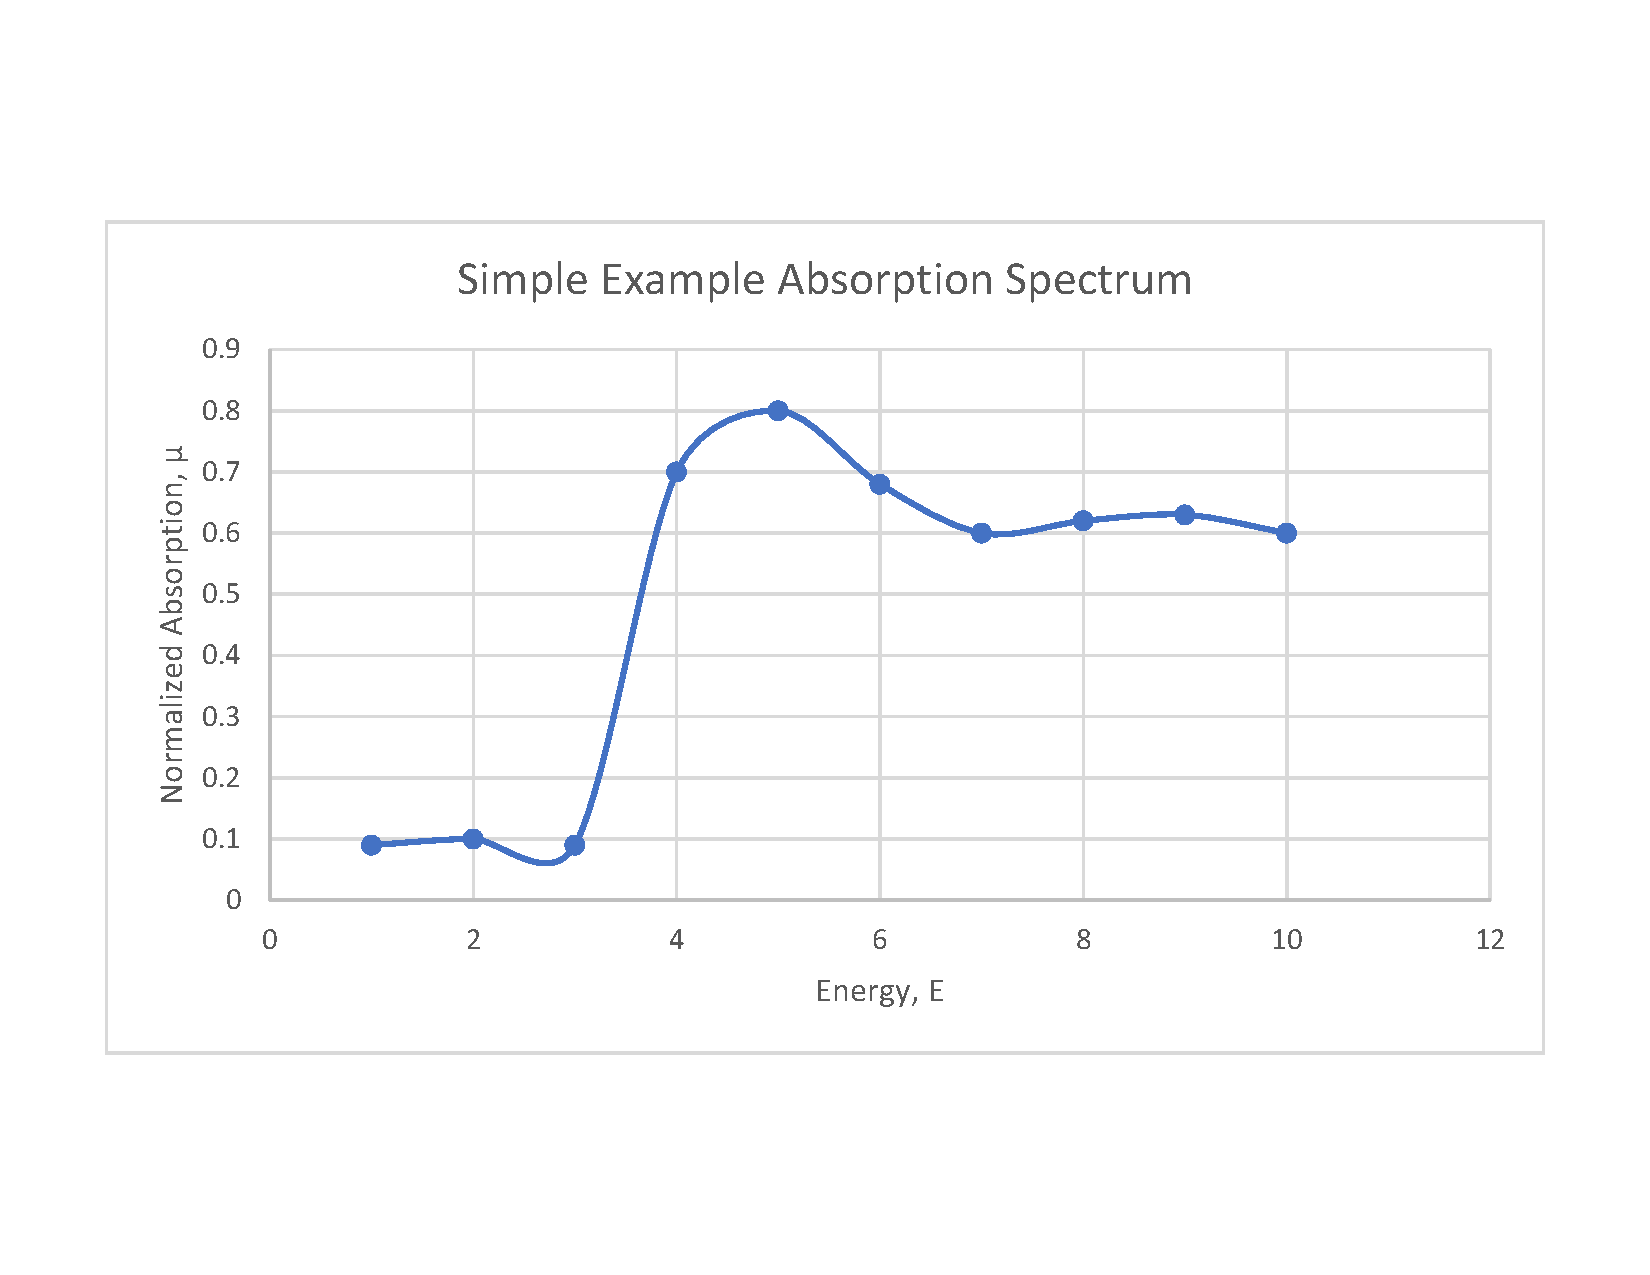
\includegraphics[width=.75\linewidth]{Chapters/Figures/conv-example.pdf}
    \caption[Toy Absorption Spectrum]{A simple abosrption spectrum for demonstration purposes.}
    \label{fig:conv-ex-spectrum}
\end{figure}
 
\noindent Each data point, $ (E, \mu) $ in the spectrum is described as a feature vector, where the feature is the the energy value for a given point $ (E, \mu) $. The vector, $ f $,  is depicted below with boxes to represent each element in the vector. Zeros are padded on both sides for reasons that will become clear soon. 

\begin{table}[h!]
    \centering
    \begin{tabular}{c|c|c|c|c|c|c|c|c|c|c|c|c|}
    \cline{2-13}
    \textit{f} = & 0 & .09 & .10 & .09 & .70 & .80 & .68 & .60 & .62 & .63 & .60 & 0 \\ \cline{2-13}
    \end{tabular}
\end{table}

\noindent Additionally, consider the kernel, $ g $  

\begin{table}[h!]
\centering
    \begin{tabular}{lccc}
    \cline{2-4}
    \multicolumn{1}{l|}{\textit{g} =} & \multicolumn{1}{c|}{.1} & \multicolumn{1}{c|}{.1} & \multicolumn{1}{c|}{.1} \\ \cline{2-4}                 
    \end{tabular}
\end{table}

\noindent The convolution works by mutliplying each element in the input vector $ f $ by the corresponding element in the kernel $ g $ and summing the results. The kernel then moves to be centered around the next element in $ f $. One way to think about this process is a kernel or filter sliding over an input signal. Applying the kernel $ g $ onto the first index of $ f $ yields: 

\begin{table}[h!]
    \centering
    \begin{tabular}{|c|c|c|c|c|c|c|c|c|c|c|c|}
    \hline
    0  & .09 & .10 & .09 & .70 & \multicolumn{1}{c|}{.80} & \multicolumn{1}{c|}{.68} & \multicolumn{1}{c|}{.60} & .62 & .63 & .60 & 0 \\ \hline
    .1 & .1  & .1  &     &     &                          &                          &                          &     &     &     &   \\ \hline
    \end{tabular}
\end{table}
$$ 
h(1) = (0)(.1) + (.09)(.1) + (.10)(.1) = 0.019
$$

\noindent where $ h(1) $ is 1st index of the resulting vector. For the next point, the kernel shifts to be centered around it. 

\begin{table}[h!]
    \centering
    \begin{tabular}{|c|c|c|c|c|c|c|c|c|c|c|c|}
    \hline
    0 & .09 & .10 & .09 & .70 & \multicolumn{1}{c|}{.80} & \multicolumn{1}{c|}{.68} & \multicolumn{1}{c|}{.60} & .62 & .63 & .60 & 0 \\ \hline
      & .1  & .1  & .1  &     &                          &                          &                          &     &     &     &   \\ \hline
    \end{tabular}
\end{table}

$$ 
h(2) = (.09)(.1) + (.10)(.1) + (.09)(.1) = 0.028
$$

\noindent The final resulting vector is:

\begin{table}[h!]
    \centering
    \begin{tabular}{c|c|c|c|c|c|c|c|c|c|c|}
    \cline{2-11}
    \textit{h} = & .019 & .028 & .089 & .159 & .218 & .208 & .190 & .185 & .185 & .123 \\ \cline{2-11} 
    \end{tabular}
\end{table}

\begin{figure}[h!]
    \label{fig:conv-res-spectrum}
    \centering
    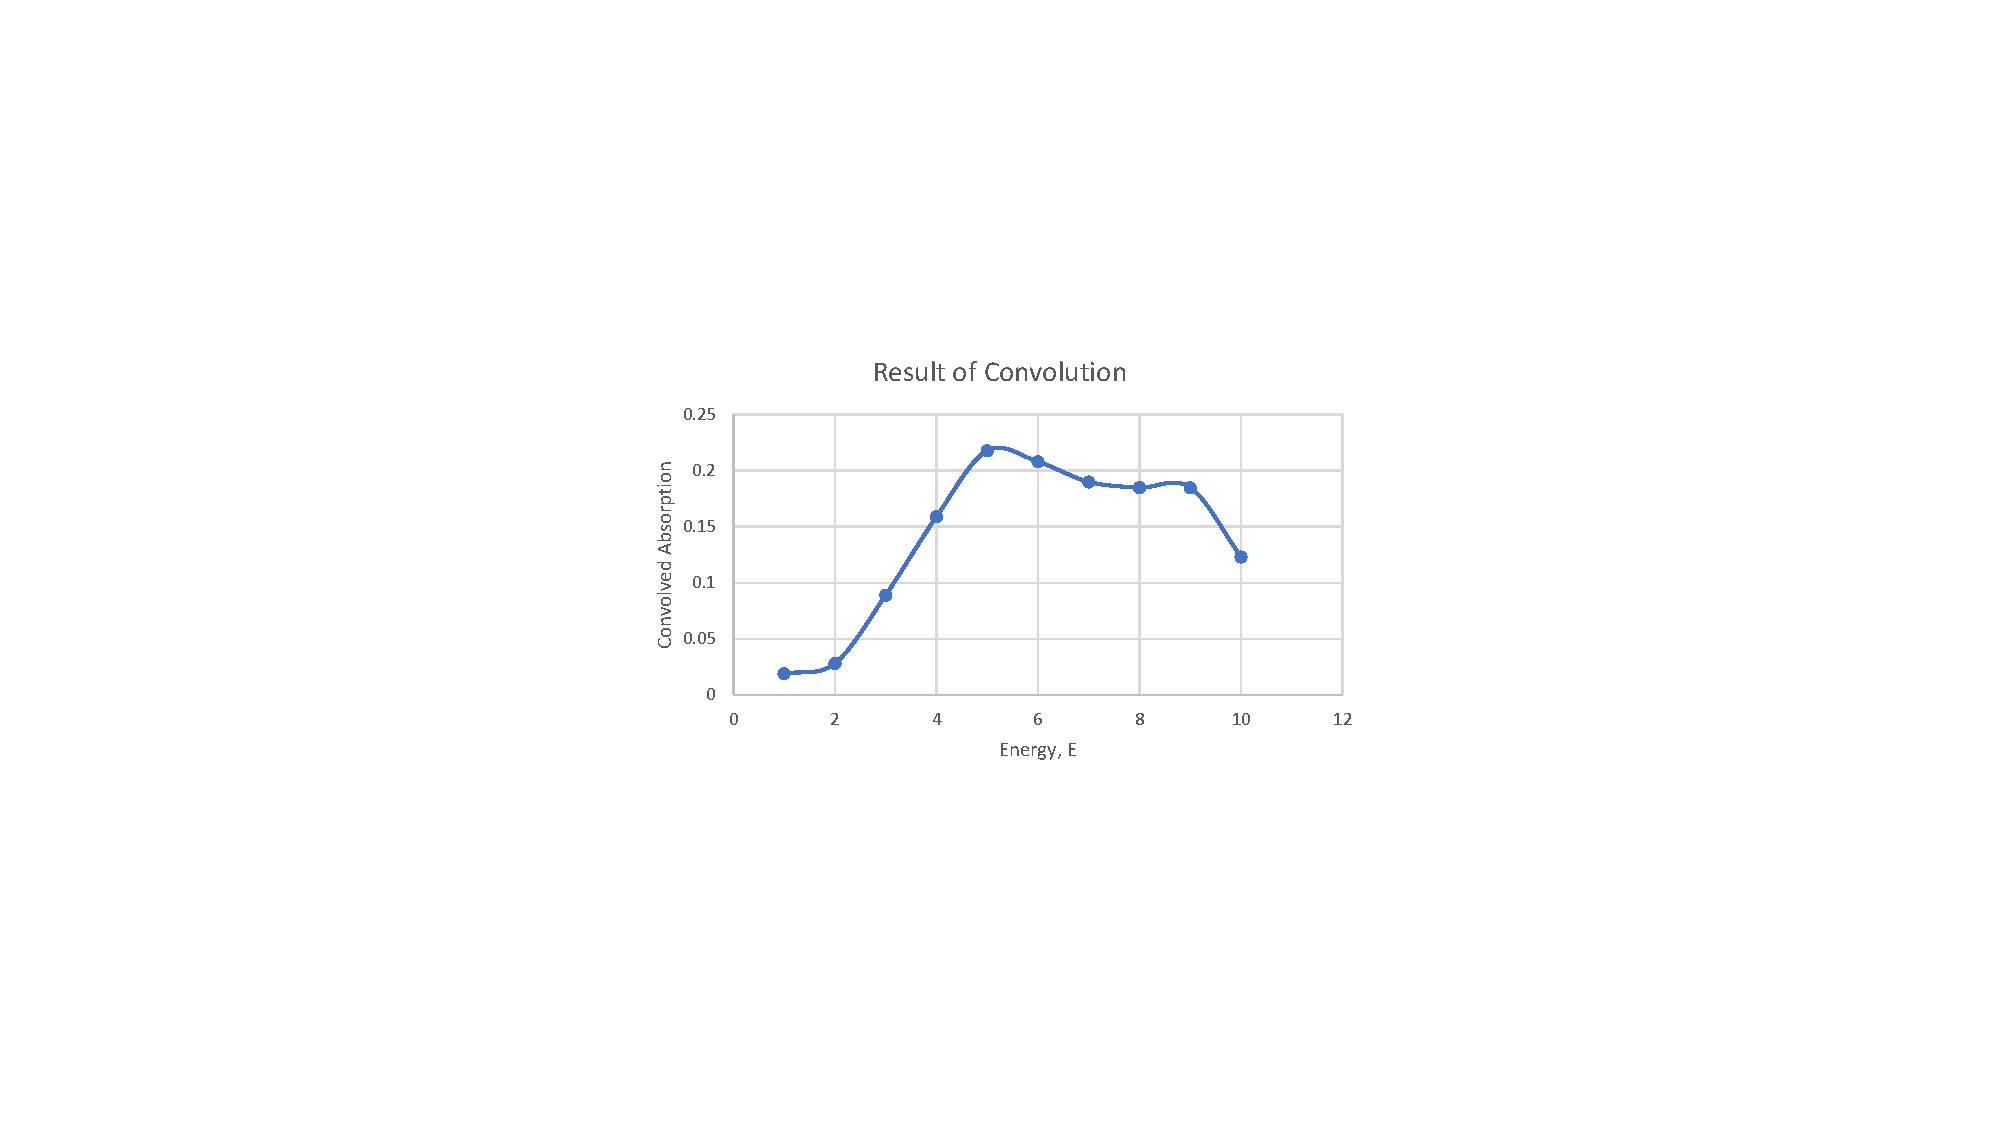
\includegraphics[width=.75\linewidth]{Chapters/Figures/conv-example-res.pdf}
    \caption[1D Convolution Result]{The result of the 1D convolution of kernel $ g = (.1, .1, .1) $  on the spectrum in Figure \ref{fig:conv-ex-spectrum}.}
\end{figure}

The toy example was chosen to demonstrate the basics of a 1D convolution. In this example, the input spectrum was a vector of length ten and the kernel of length three. In the context of applying a 1D convolution to a neural network, the size of the input vector is the cardinality of the hidden layer directly preceding the convolutional layer. Often the hidden layer's output, represented as a vector, is reshaped into an n-dimensional tensor before applying the convolution. To apply a 1D-convolution to a Tensor of rank $ n $, simply apply the convolution to each of the n-vectors separately, ensuring to pad the ends of each vector with zeros. Layers with dimensionality greater than one can be ``un-raveled''. Alternatively, the layers of each dimension can be truncated or ``pooled'' by averaging the layers that are stacked on one another (or taking the max of each layer) until the desired dimensionality is achieved. A common way to achieve this is with a max pooling layer or an average pooling layer. Max pooling and average pooling layers also have the additional benefit of downsampleing the feature space, tending to make the network more robust to slight variations in the position of features in the input image or signal. This is referred to as ``local translation invariance'' \cite{local-translation-invariance}.

Another important possible change in the above example is the stride length. In the above example, we ``slid'' the kernel across the input spectrum one point at a time. This is referred to as a stride size or stride length of one. The stride could be any integer less than the length of the input vector $ f $, though in practice, typically stride lengths tend to be one or close to one. Lastly, in the above example, we only applied one convolutional kernel, or ``filter.'' In practice, many filters are applied sequentially. In the above example, the filter $ g = (.1, .1, .1) $ was simply decided upon \textit{a priori}. In practice, the values for each filter in the convolutional layer are initialized randomly or according to the specified initialization function. The default in Keras is Glorot Uniform. The values of each filter are trainable parameters that evolve to produce the best final prediction given the subsequent layers in the neural network.


\section{How to Train a Neural Network}
Building a successful neural network requires a combination of intuition and procedural know-how. The first key is to start with a simple model, perhaps a single hidden. If you start with a complex model with data augmentation and regularization, you’ll never be able to tune the hyperparameters and find a good solution. Then, a good strategy is to pick a simple architecture and reasonable hyperparameters and train the model on a small subset of training samples, say 1--10 samples. Train the model over 10 or so epochs and see if the training cost is decreasing and see if you can overfit. If you can overfit the small sample size, it means the code is working and the network architecture makes sense. Now you can increase the number of samples in the training data, either to the full train-test split or a subset of that if working with ``big data.''\footnote{Big data has become a nebulous term, but a reasonable example is when you there is so much data that the dataset cannot be loaded into the computer's memory (RAM) at the same time.} Next, you can run a broad hyperparameter search. Afterward, run maybe 20 epochs and see how the training and validation loss is moving. If they both are going down, the architecture looks good. If not, start over. Ideally, the training and validation loss curves will be decreasing together like in figure \ref{fig:Example-Training-Loss-Curve}. If the model still does not predict well after hyperparameter tuning, the model is underfitting, and a more complex architecture is required (add more layers).

\begin{figure}
    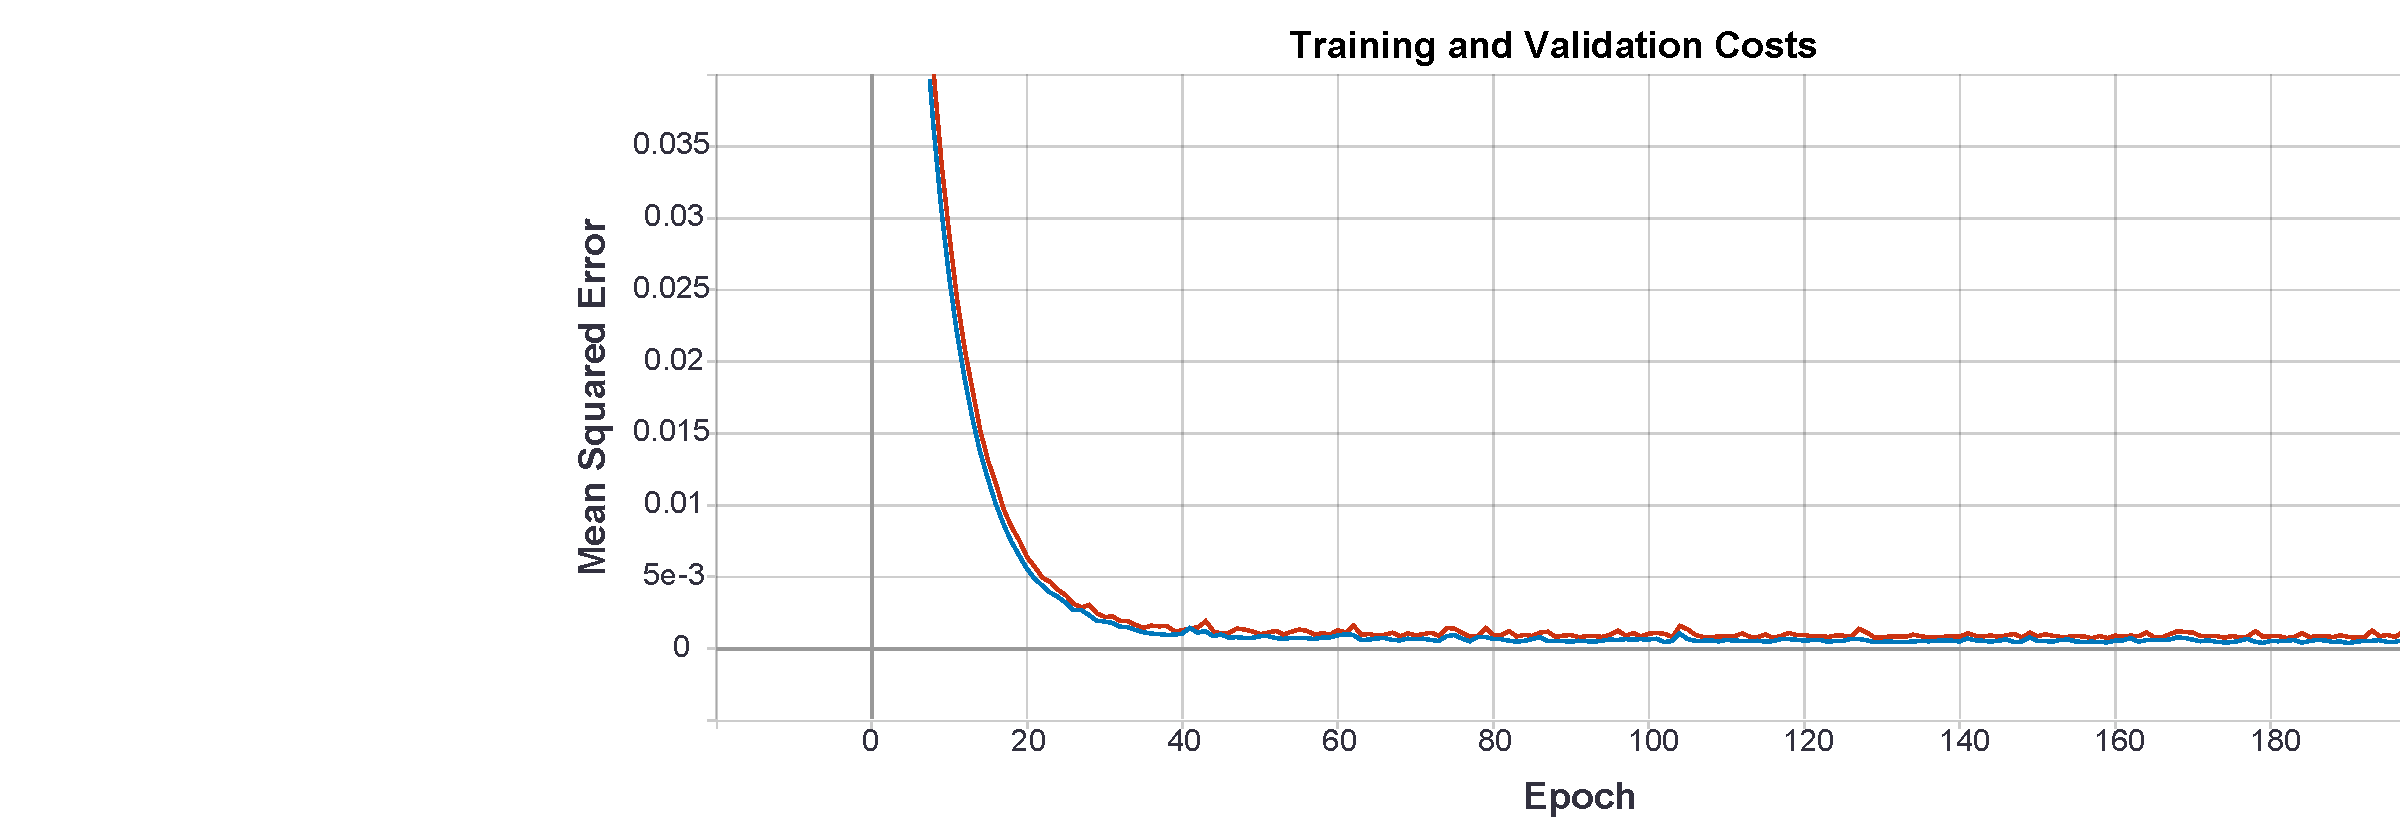
\includegraphics[width=\linewidth]{Chapters/Figures/epoch_loss1.pdf}
    \caption[Example ANN Training Curve]{In this example loss curve, the x-axis is the epoch, and the y-axis is the mean-squared error of the prediction. The red curve is the training data, and the blue curve is the validation set. Notice how both curves decrease together, but the training curve has a smaller error than the validation curve. This is the expected behavior of a model that is not overfitting and training properly.}
    \label{fig:Example-Training-Loss-Curve}
\end{figure}

Ideally the training and validation loss will decrease together over many epochs. It is likely, however, that after many epochs the training loss will continue to decrease while the validation loss plateaus. This is the point to start introducing regularization such as dropout layers as well and considering data augmentation. These techniques will allow the model to continue decreasing the validation loss and prevent overfitting. The main goal of training is to minimize the validation loss. The placement of dropout layers and the type of data augmentation are subject to trial and error. Generally, it is best to include dropout layers after a ReLU acticaiton and before an affine layer, and there has been some research suggesting the inclusion of low-probability dropout layers after convolutional layers tends to improve model performance \cite{conv-dropout-layers} \cite{conv-dropout-layers2}, but these rules do not work for every network and it is still worth trying different options while training.



% \section{Autoencoders if they become useful}
% Talk about how autoencoders work. Give a nice broad explanation and really go into the math. Include some nice diagrams

% Here's \cite{ng2011sparse} a good source to read and model off of. Here \cite{Bhowick2019} is another paper that might be interesting to read. It's about getting noise-free data from the original data using an autoencoder. Neat idea, and could actually be very relevant because they're using geophysical data.





\chapter{Results}
% Results
The results of the raining process are presented in this chapter. We begin by first solving outlining the training network architecture and training process on simulated XANES in section \ref{sec:nn-sim-data}. Then, we discuss the work on expanding the model to make solid predictions on experimental data.

\section{Training with Simulation Data} \label{sec:nn-sim-data}
The 1000 simulated XANES spectra were first loaded into a Pandas dataframe \cite{pandas-1} \cite{pandas-2} of shape $ 1000\times82 $. Each of the 82 columns represents a discrete energy value, and each row represents the absorption for a given spectrum at those energies. The dataset was split into training and testing groups according to an 80-20 random split, respectively. All absorption columns were then scaled via the standard scalar (\ref{z-score}) and the training labels scaled via a min-max scaler (\ref{eqn:min-max-scaler}). First, the model was trained to predict four descriptors: the mean-squared-displacement (MSD), the mean bond length distance, the standard deviation of the bond length distributions, and the skew of the bond length distribution. Note that the standard deviation is the same as the square root of the MSD. This feature was only included preliminarily in order to better understand the correlation in the network's predictions. 

\bgroup
\def\arraystretch{1.5}%  1 is the default, change whatever you need
\begin{table}[h!]
    \centering
    \begin{tabular}{|l|l|l|}
    \hline
    Layer  Type    & Output Shape  & Number of Parameters \\ \hline
    Normalization  & (None, 82)    & 165                  \\ \hline
    Dense          & (None, 128)   & 10,624               \\ \hline
    Dense          & (None, 128)   & 16,512               \\ \hline
    Dense          & (None, 512)   & 25,088               \\ \hline
    Reshape        & (None, 8, 64) & 0                    \\ \hline
    1D-Convolution & (None, 6, 32) & 6,176                \\ \hline
    Dropout        & (None, 6, 32) & 0                    \\ \hline
    1D-Max-Pooling & (None, 3, 32) & 0                    \\ \hline
    Flatten        & (None, 96)    & 0                    \\ \hline
    Dense          & (None, 128)   & 12,416               \\ \hline
    Dense          & (None, 48)    & 6,192                \\ \hline
    Dense          & (None, 512)   & 25,088               \\ \hline
    Flatten        & (None, 512)   & 0                    \\ \hline
    Dense          & (None, 4)     & 513                  \\ \hline
    \end{tabular}
    \caption[NN-Architecture Optimized for Simulations]{The model architecture for the network trained entirely on simulation data (which performed poorly on experimental data) relies primarily on affine (Dense) and convolutional layers. The model includes 108,966 total parameters, with 108,801 of those being trainable.}
    \label{tb:nn-arch-sims}
\end{table}
\egroup


\begin{figure}
    \centering
    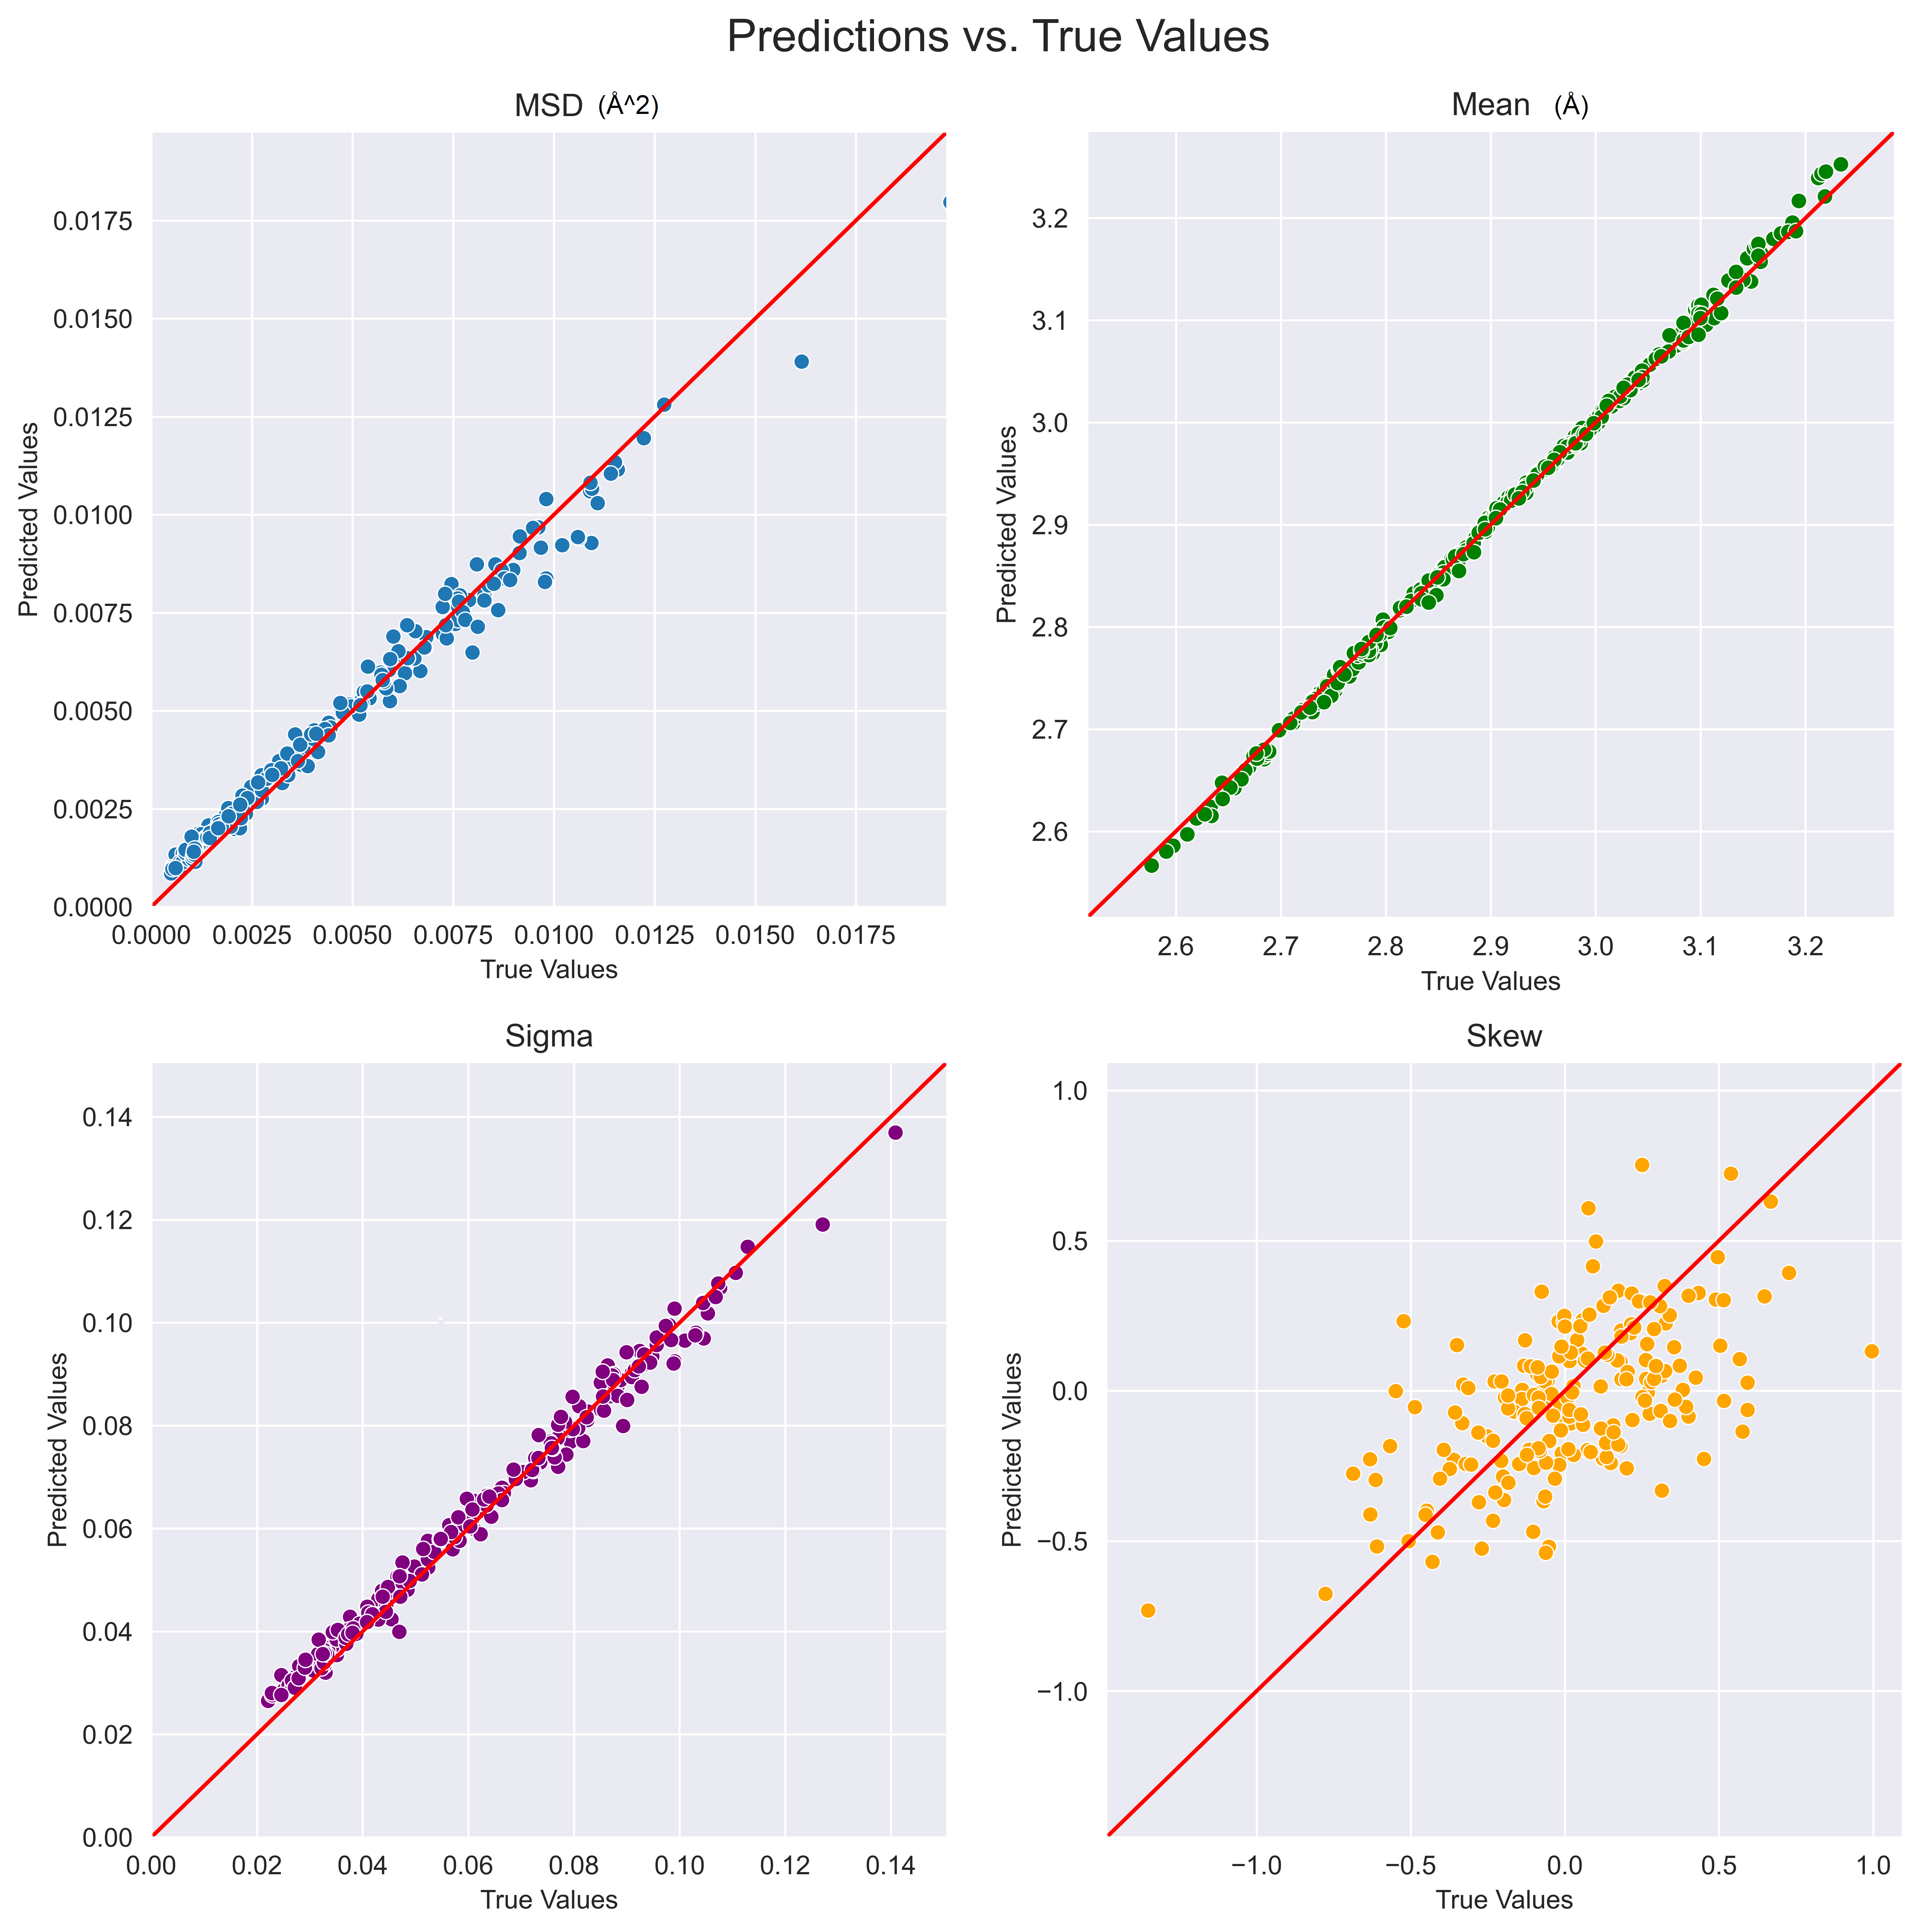
\includegraphics[width=\linewidth]{Chapters/Figures/pa_train-test-fixed.png}
    \caption{One configuration of the trained neural network includes four output nodes: MSD, Sigma, Mean, and Kurtosis. Sigma is just the square root of the MSD and was included during training to confirm the patterns recognized by the network. Each point in each subplot represents a FEFF simulated spectrum in the test set. For each spectrum, the y-axis represents the MSD value predicted by the NN, and the x-axis represents the true MSD (label) for that spectrum. Hence, points on the $ y=x $ red line are perfect predictions.}
    \label{fig:train-test-split-all4}
\end{figure}

\section{Experimental Data} \label{ch:results}

Training the neural network entirely on simulation data and then making predictions on experimental data is unlikely to provide quality results. Using the trained network from Table (\ref{tb:nn-arch-sims}) that predicted the test set values in Figure \ref{fig:train-test-split-all4}, we predicted the MSD values from two experimental spectra. On the unpublished IMASC data, the network predicted an MSD of $0.0003724~\AA^2$ instead of the EXAFS equation fitted value of ${\sigma^2=0.0102(8)~\AA^2}$. This poor prediction suggests the network considers the experimental spectrum to look most similar to the lowest disorder FEFF spectra; the model is not generalizing to understand the disorder encoded in the spectral shape.


\begin{figure}
    \centering
    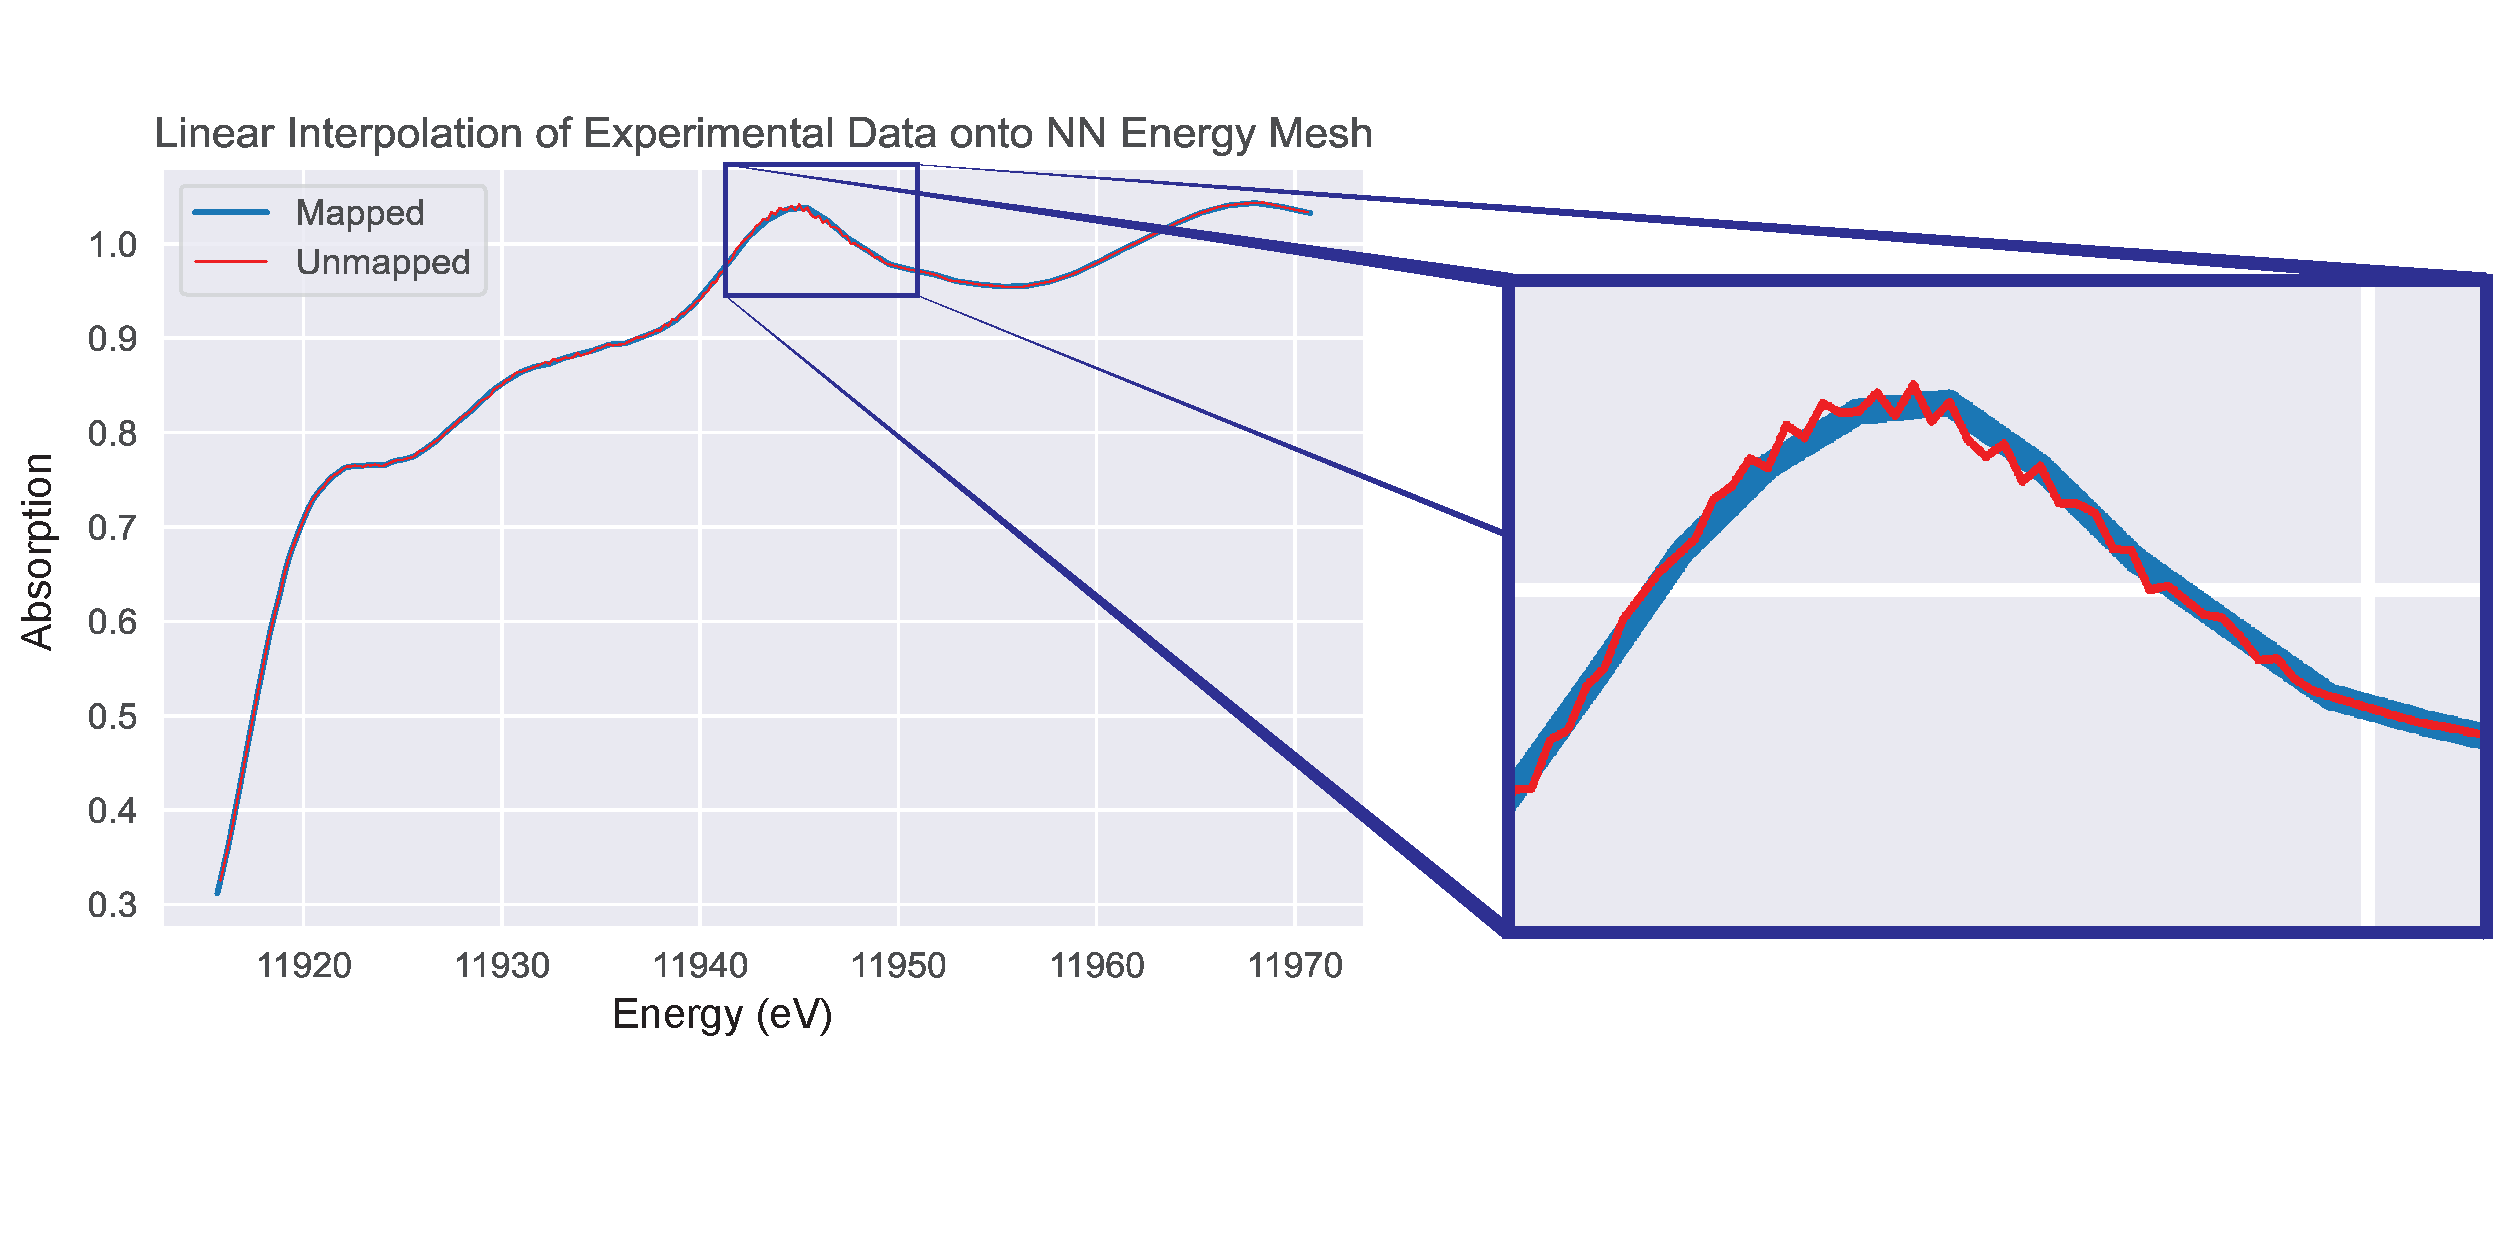
\includegraphics[width=\linewidth]{Chapters/Figures/quality-of-interpolation-skinny.pdf}
    \caption[Experimental Data Interpolation]{The experimental data is measured as a function of different energy values than the ones on which the neural network is trained. Consequently, the experimental spectrum must be mapped onto the proper energy mesh via linear interpolation.}
    \label{fig:interpolation-skinny}
\end{figure}

\subsection{Data Augmentation}
While there is ample data for training and predicting on only simulation data, we only have two experimental spectra. In order to create more training and testing data for the neural network, two types of data augmentation were utilized: horizontal spectral shifting and Gaussian noise inclusion. While the motivation for utilizing data augmentation is to expand the size of the experimental training and testing set, the neural network must be trained to recognize the augmentation types prior to training or testing on the experimental data. As such, both the FEFF simulated dataset and experimental dataset are augmented.

Noise is artificially injected into the spectra by randomly shifting each absorption coefficient vertically. The shifted value for each energy level is selected from a Gaussian distribution with standard deviation $ \sigma=0.01 $. An exaggerated example of the injected noise is shown in Figure \ref{fig:data-aug-gauss-noise}.

\begin{figure}[h!]
    \centering
    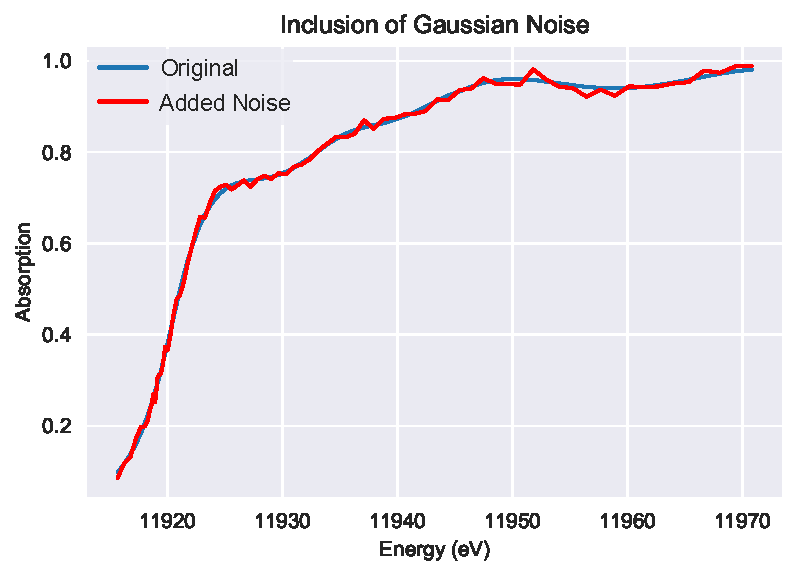
\includegraphics[width=.75\linewidth]{Chapters/Figures/gaussian-noise-data-aug.pdf}
    \caption[Data Augmentation: Gaussian Noise]{Gaussian noise is added to the spectra to increase the variance of the training data. This helps the network to learn the low-level features of the spectra and ignore artifacts not caused by the structural disorder. For demonstration purposes, the scale of the noise in this figure has been increased beyond what was used in training.}
    \label{fig:data-aug-gauss-noise}
\end{figure}

The second form of data augmentation utilizes horizontal shifts. While this is common for signal processing and time series analysis, the inclusion here is more controversial. In XAFS, the edge location is dependent on the oxidation/reduction state of the species. Shifting the horizontal location is akin to shifting the species of the model; however, the neural network is not being tasked to determine the oxidation state of the sample. Instead, the model is only tasked with predicting the mean-squared-displacement of the nanoparticle's bond lengths. The theory is that the disorder information is encoded in the  

\begin{figure}[h!]
    \centering
    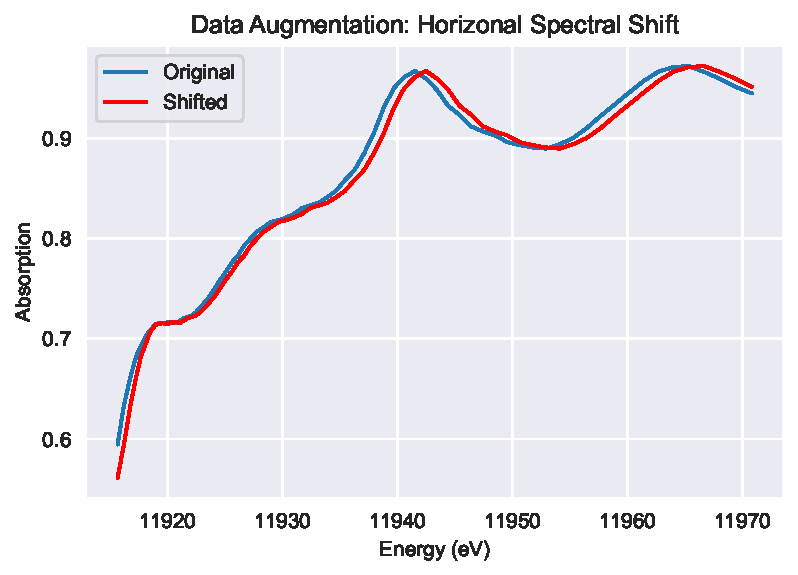
\includegraphics[width=.75\linewidth]{Chapters/Figures/data-aug-shift-pt75wieght.pdf}
    \caption[Data Augmentation: Horizontal Shift]{In order to train the network to predict disorder from the overall shape of the spectra---as opposed to fixating on the edge location---we introduce horizontal-shift as a data augmentation technique.}
    \label{fig:data-aug-hor}
\end{figure}

\subsection{Transfer Learning}
In building the transfer learning model, we opted to begin with a new network architecture, which can be found in Table (\ref{tab:meta-1}). We hypothesized that applying convolutional layers before any affine layers may lead to a more consistent prediction between simulation and experimental spectra.

\begin{figure}
    \centering
    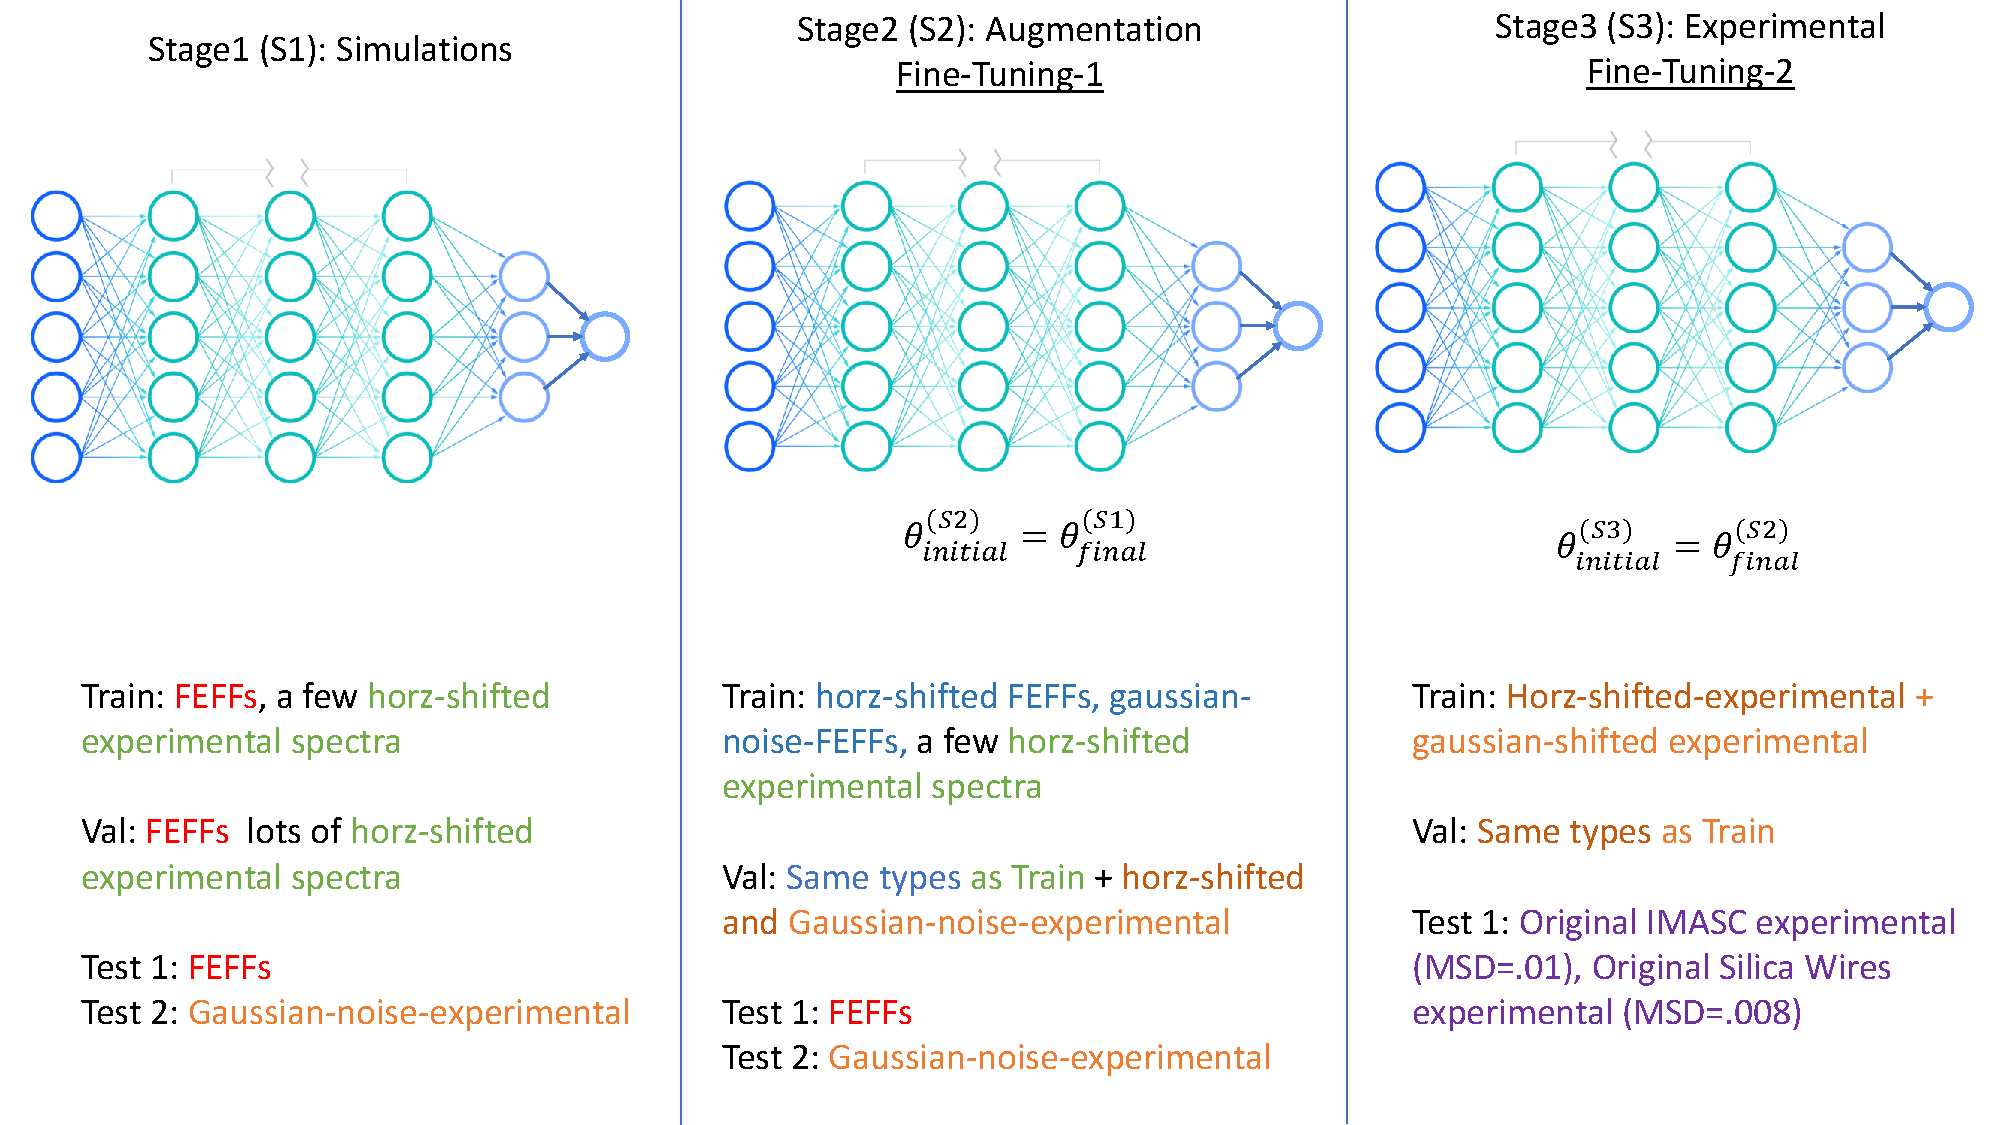
\includegraphics[width=\linewidth]{Chapters/Figures/transfer-learning-breakdown.pdf}
    \caption[Transfer Learning Process]{Caption here}
    \label{fig:transfer-learning-databreakdown}
\end{figure}

\bgroup
\def\arraystretch{1.5}
\begin{table}[]
    \centering
        \begin{tabular}{|l|l|l|l|}
        \hline
        \multicolumn{1}{|c|}{\textbf{Name}} & \multicolumn{1}{c|}{\textbf{Type}} & \multicolumn{1}{c|}{\textbf{\# Parameters}} & \multicolumn{1}{c|}{\textbf{Output Shape}} \\ \hline
        normalization\_input                & InputLayer                         & 0                                           &                                            \\ \hline
        normalization                       & Normalization                      & 165                                         & None, 82                                   \\ \hline
        reshape                             & Reshape                            & 0                                           & None, 82, 1                                \\ \hline
        conv1                               & Conv1D                             & 128                                         & None, 82, 32                               \\ \hline
        max\_pooling1d                      & MaxPooling1D                       & 0                                           & None, 41, 32                               \\ \hline
        conv2                               & Conv1D                             & 3104                                        & None, 39, 32                               \\ \hline
        max\_pooling1d\_1                   & MaxPooling1D                       & 0                                           & None, 19, 32                               \\ \hline
        flatten                             & Flatten                            & 0                                           & None, 608                                  \\ \hline
        dense1                               & Dense                              & 58464                                       & None, 96                                   \\ \hline
        dout                                & DropOut                            & 0                                           & None, 96                                   \\ \hline
        dense2                              & Dense                              & 30264                                       & None, 312                                  \\ \hline
        output                              & Dense                              & 313                                         & None, 1                                    \\ \hline
    \end{tabular}
    \caption{A new network architecture was constructed for the transfer learning process. The new network only has one output node, representing the MSD of the input spectrum.}
    \label{tab:meta-1}
\end{table}
\egroup

Our approach to succesfully applying transfer learning involves two stages of fine-tuning. First, we primarily  train the model on FEFF simulated spectra, selecting an architecture and hyperparameters which are likely to be compatible with fine-tuning. We achieve this by weighting the validation set heavily (around $ 10\% $) with augmented experimental spectra and choosing a model which performs as well predicting unseen data-augmented experimental spectra as it does predicting unseen simulated FEFF spectra. The training loss curves and selection process can be found in Figure \ref{fig:meta-1-sweep-loss}. One concern with this approach is that we are injecting biases into out model selection; however, we take this into account through utilization of a third, unseen test set, and the fact that the model does not update its parameters based on its predictions on the validation set. When training a model in machine learning, the parameters are continuously update until a minimum is reached in the loss function. While the loss function will have a global minimum, it also contains local minima, some of which will be more agnostic to the differences in experimental spectra and be better candidates for transfer learning. In this first stage of learning, the intention is to teach the model to find broad predictive features from the simulation set, while selecting a model at a local minimum which is likely to be a good transfer-learning candidate. 


\begin{figure}
    \centering
    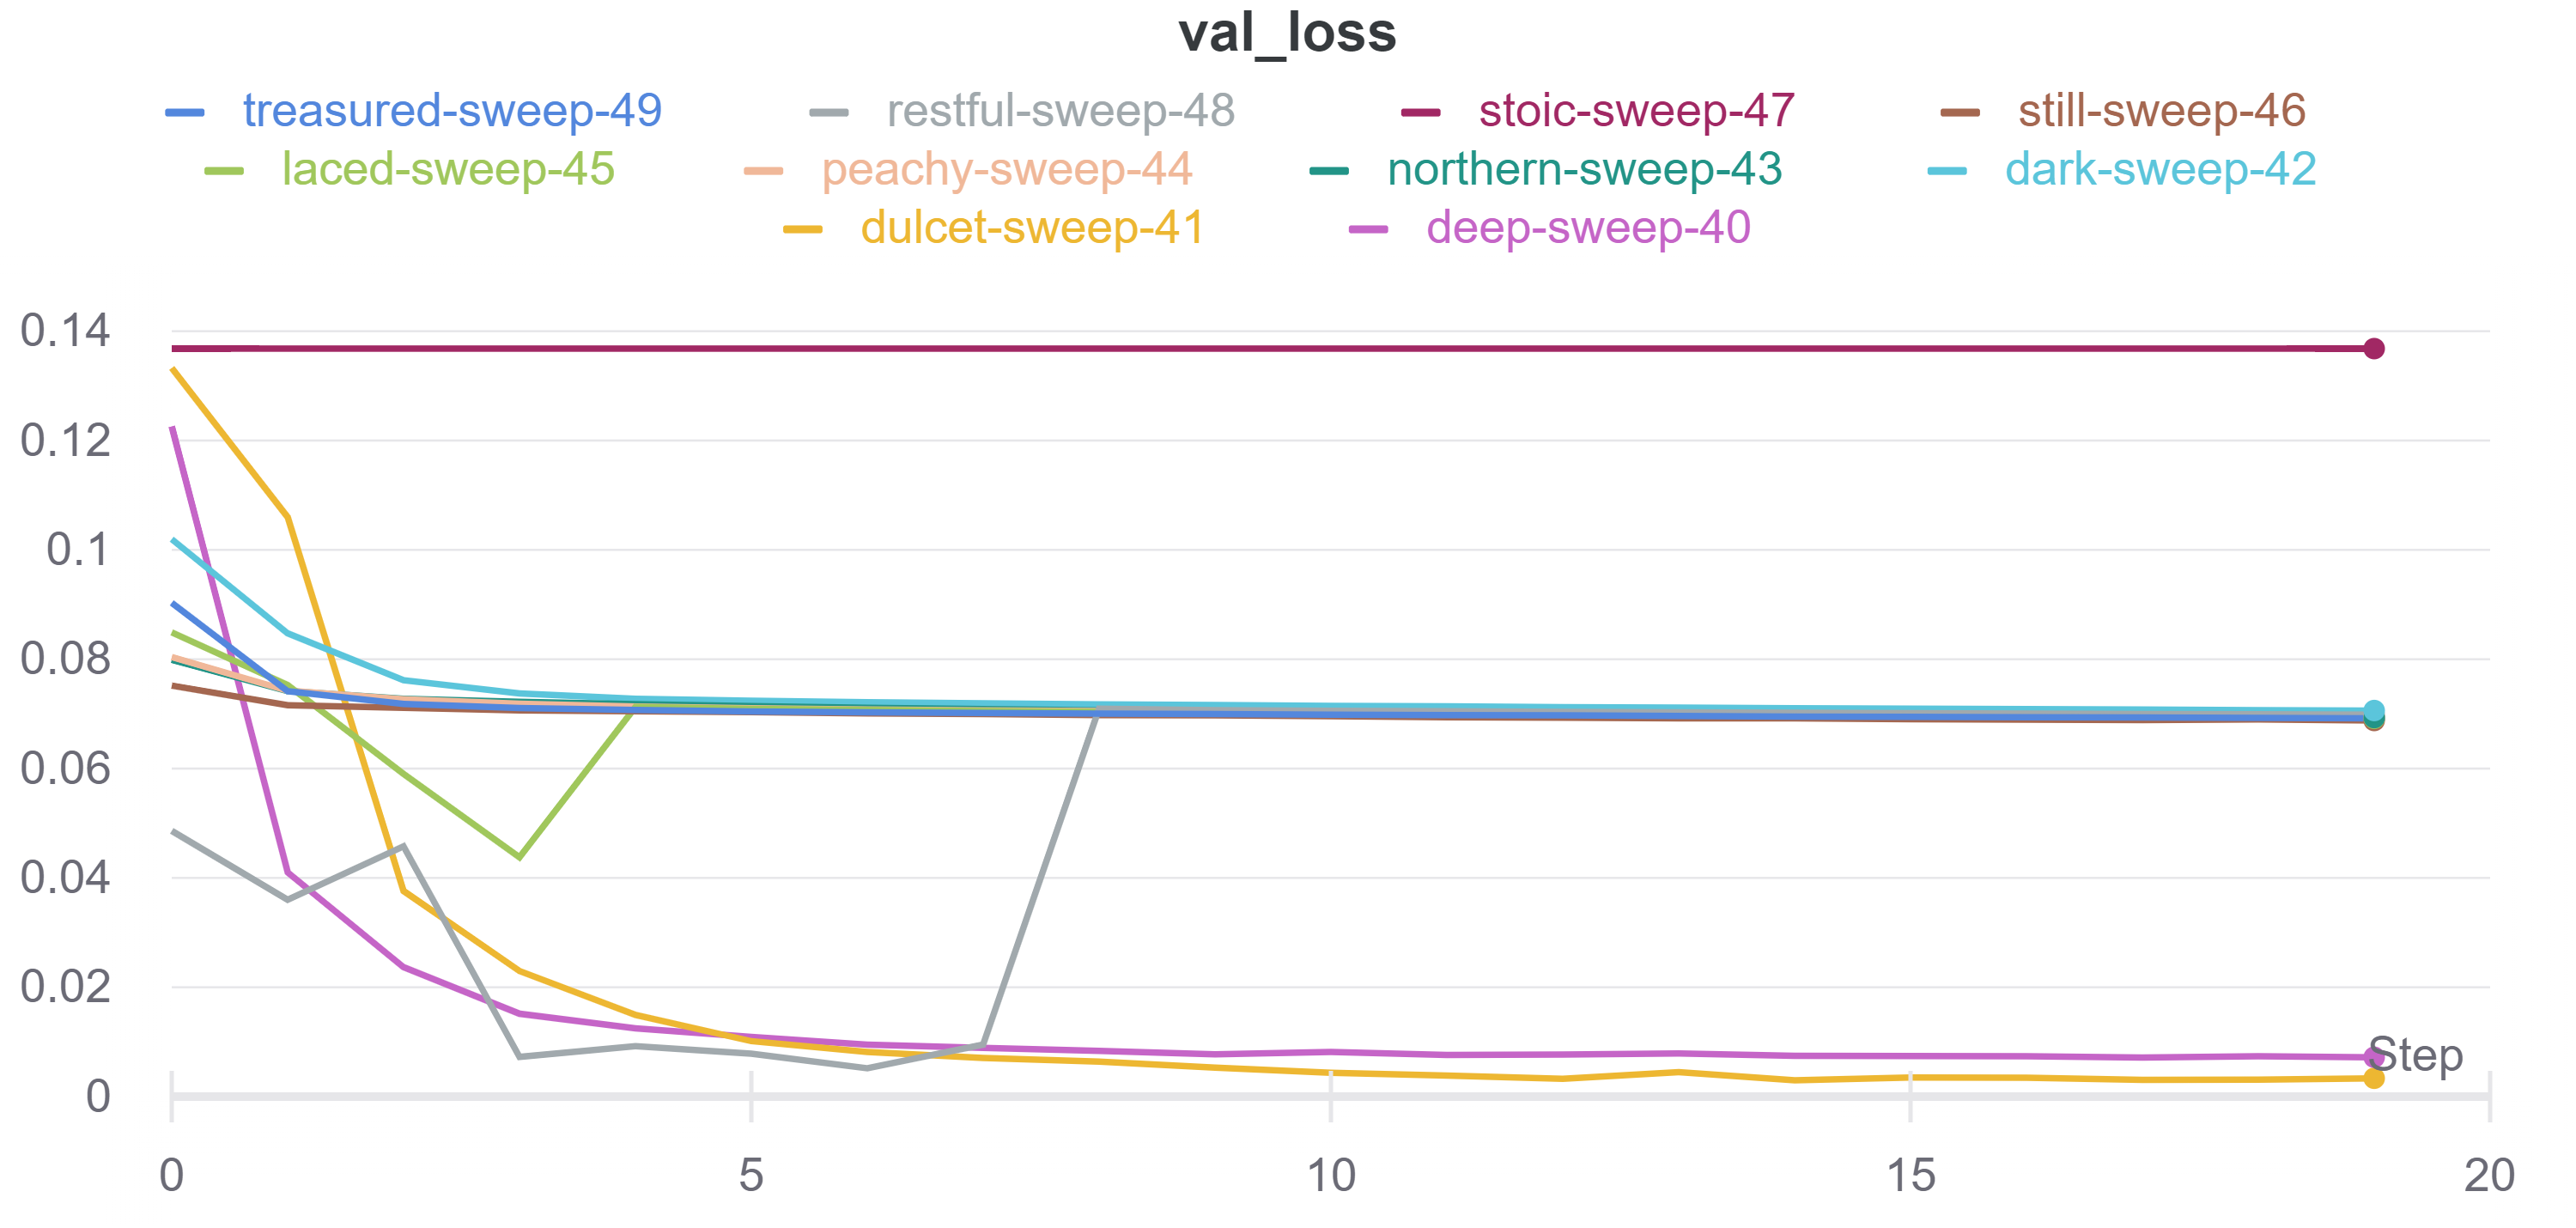
\includegraphics[width=\linewidth]{Chapters/Figures/10-sweep.png}
    \label{fig:meta-1-sweep-loss}
    \caption[Hyperpamater Sweep 1]{The validation loss (mean-squared-error) for 10 out of the 50 hyperparameter combinations searched in this sweep are plotted above. Most hyperparameters result in a loss curve stabilizing around 0.08, which is significantly higher than the training loss (not shown) that stabilized around 0.01. A few of the validation loss curves, instead, stabilized around 0.01 (dulcet-sweep-41 and deep-sweep-40). Because the validation set is heavily weighted with augmented experimental spectra, these two spectra are likely to be good candidates for transfer learning onto experimental data.}
\end{figure}

The next stage of transfer learning seeks to teach the model to ignore noise and focus on the broader shape of the spectrum. We achieve this by freezing the early stages of the model and retraining the later parameters on a new dataset comprised primarily entrirely of data-augmented spectra. Often, models are trained with the augmented dataset in the initial stage, which helps act as a form of regularization. In the case of transfer learning, however, applying this regularization so early on in the process may lead to undesirablr local minima for which transfer learning onto the experimental dataset would be impossible. By applying an initial stage of fine-tuning to a well-tuned base-model, we increase the likelyhood of a succesful second fine-tuning stage.

The last stage of the fine-tuning process is to freeze even more layers and reduce the learning rate, then train the model using all of the data-augmented experimental spectra. If the process is sucesful, the model will have learned to predict the MSD and ignore horizontal and gaussian noise in the spectra from the first stage. In this way, we have increased the number of possibly training samples to use for the final fine-tuning stage from one to many, and allowed us to withhold both of the un-altered experimental spectra from the training process and use them to evaluate the success of the transfer learning process. A visualization and specific breakdown of which data is allocated into each stage of the training process can be found in Figure \ref{fig:transfer-learning-databreakdown}.

\begin{figure}
    \centering
    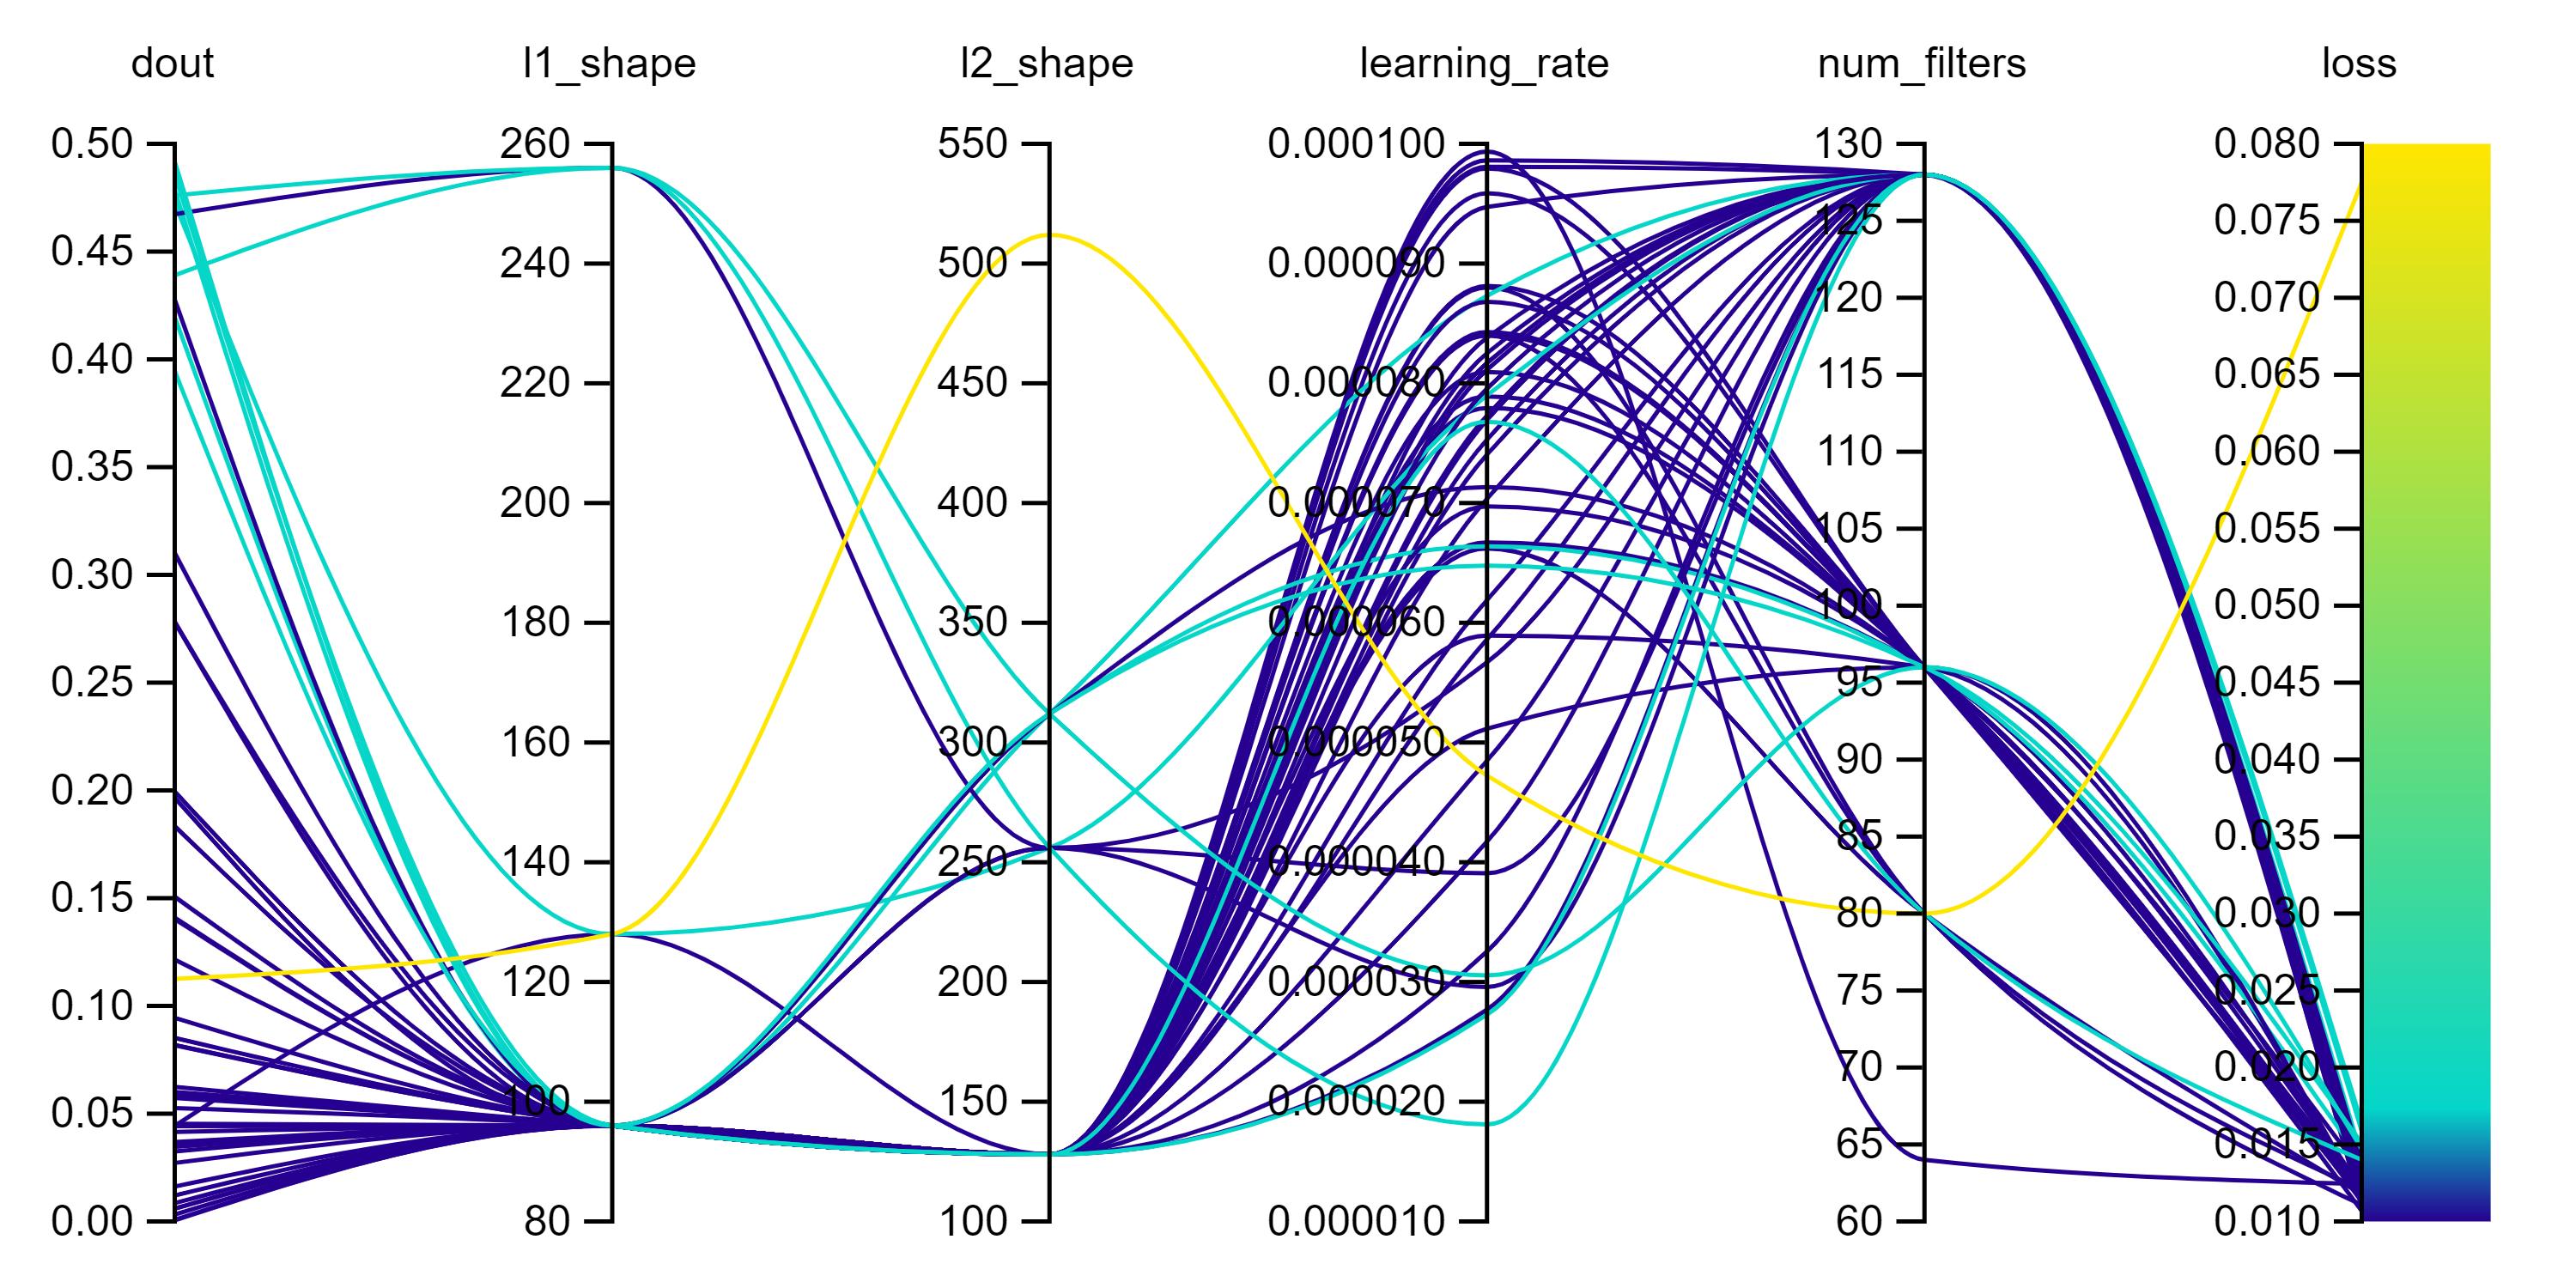
\includegraphics[width=\linewidth]{Chapters/Figures/new-hyperparameter-sweep-meta-1.png}
    \label{fig:meta-1-sweep-params}
    \caption[Hyperpamater Sweep 1]{The hyperparameters are obtained through a ``sweep,'' where the entire training process (20 epochs) is repeated with different hyperparameters each time. The hyperparameter training process and figure generation was conducted with the aid of \cite{wandb}.}
\end{figure}





\begin{figure}
    \centering
    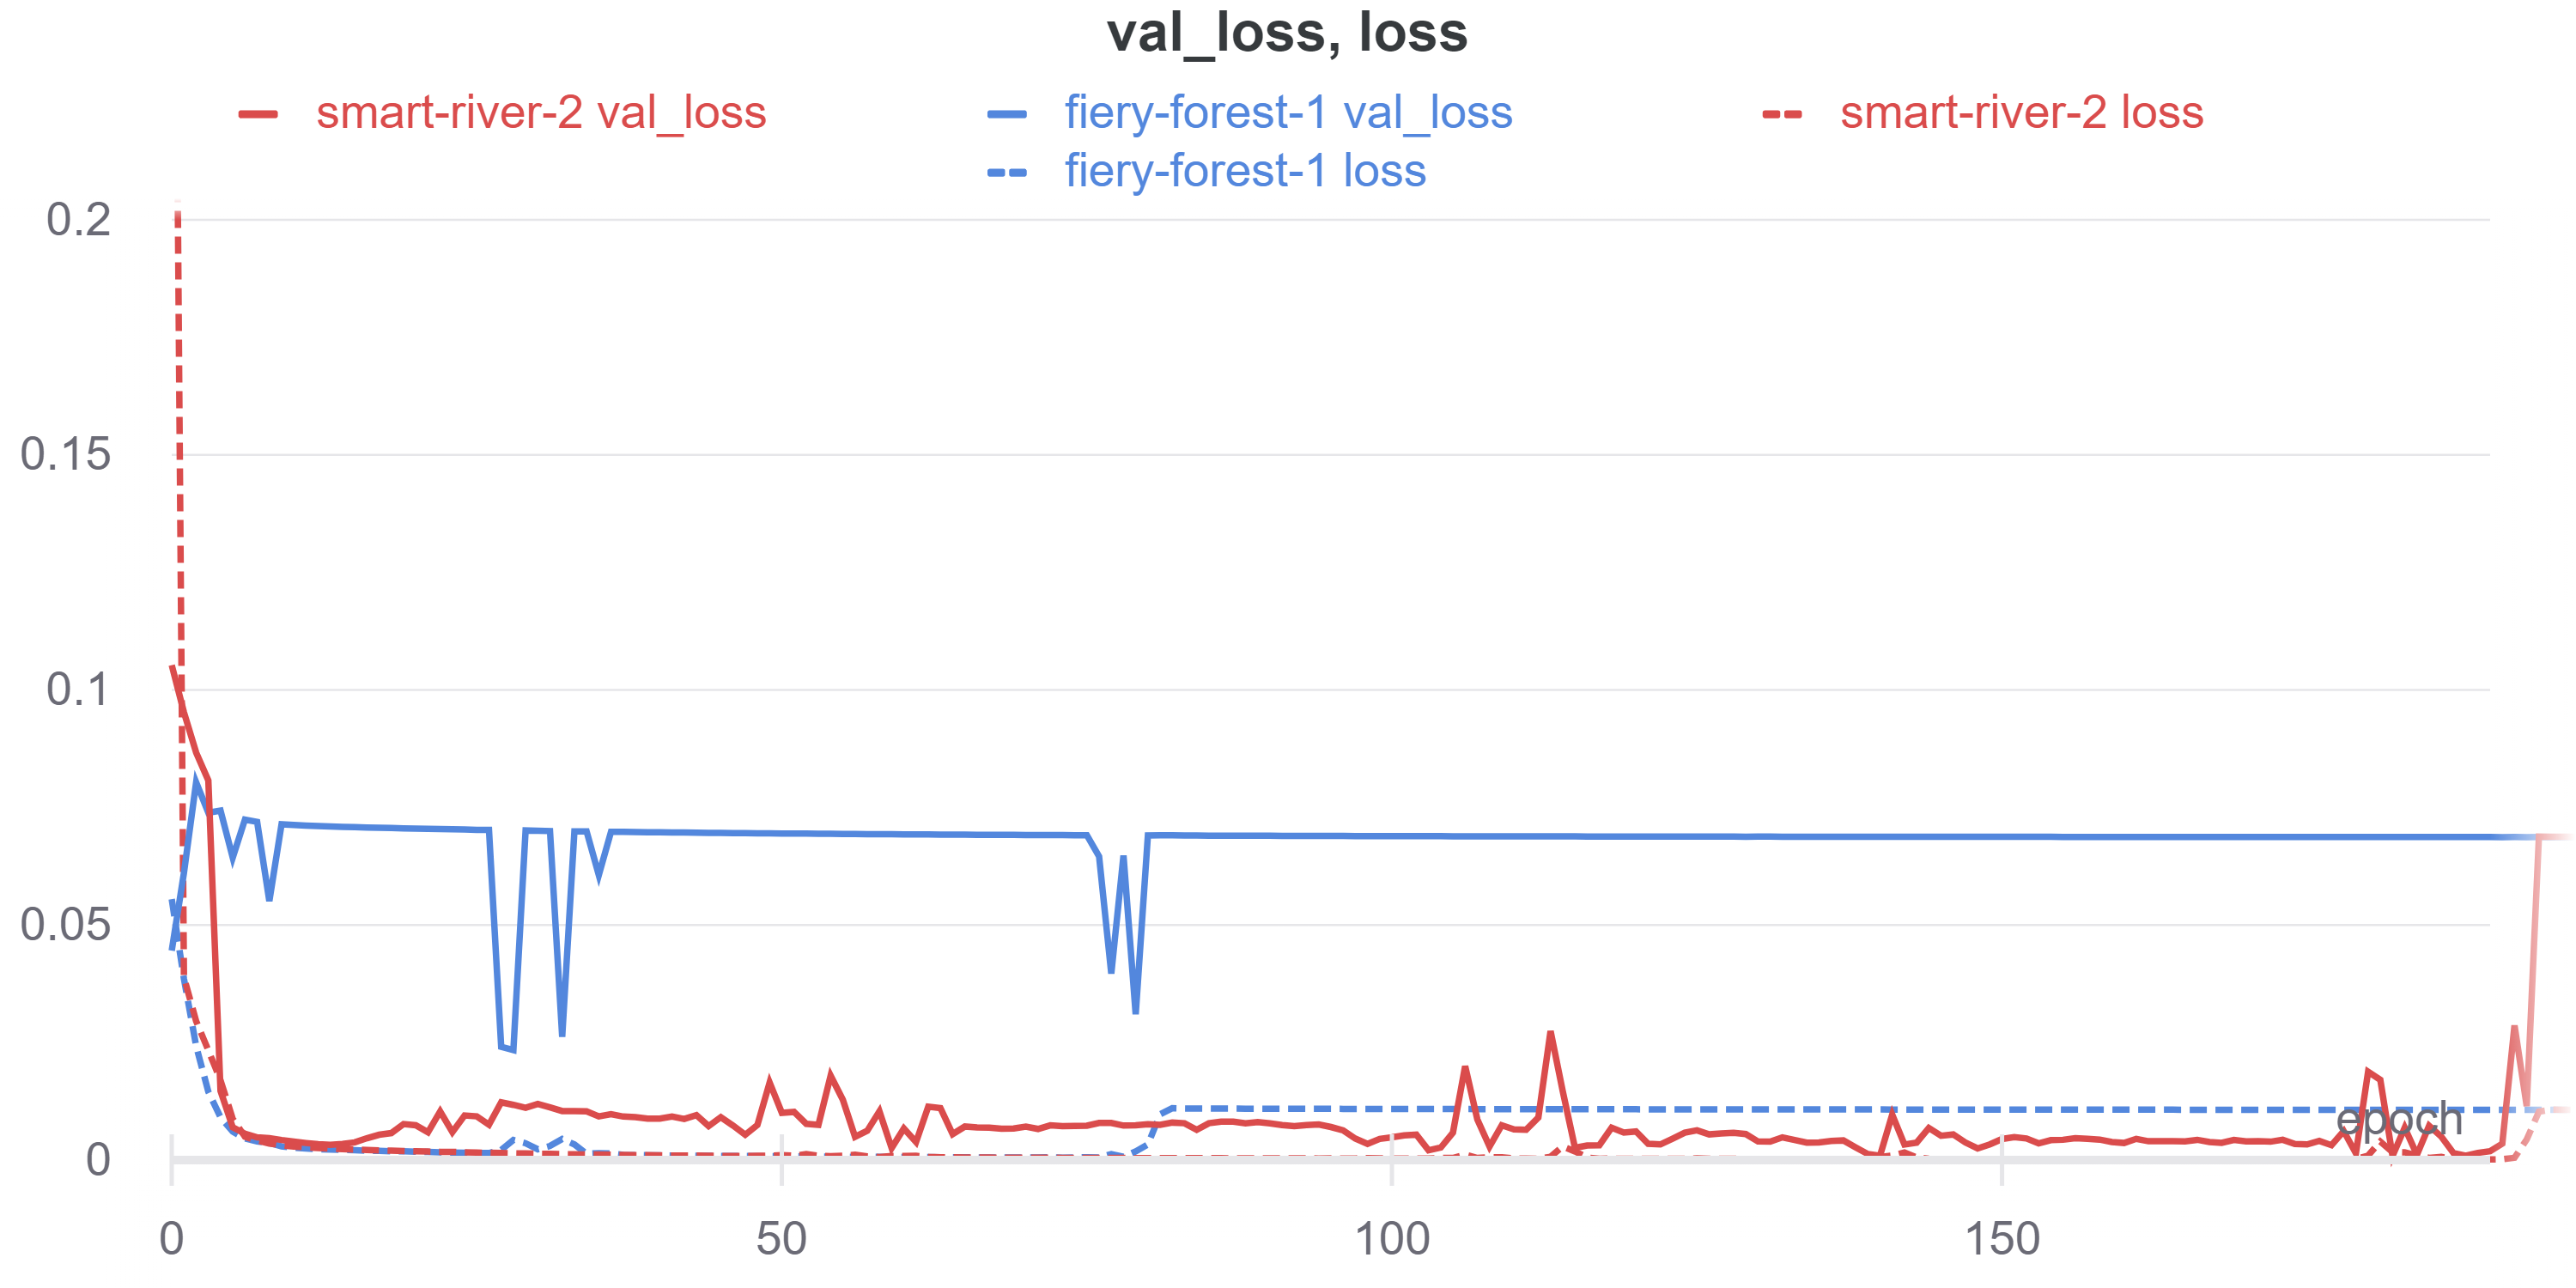
\includegraphics[width=\linewidth]{Chapters/Figures/best-params-meta1.png}
    \label{fig:meta-1-best}
    \caption[Hyperpamater Sweep 2]{Both iterations of the training process were run with identical network architectures and hyperparameters; however, the two runs have significantly different validation losses. The discrepancy is due to the random weights initialization process. We mitigate this problem by setting global random seeds throughout the training process to select consistent pseudo-random values. The slight difference in initial parameters causes one iteration to become "stuck" in a different local minimum, which performed similarly with the training set but made substantially worse predictions on the validation set. The goal of the first stage of the transfer learning process is to identify hyperparmaters which will lead to the best transfer learning candidates.}
\end{figure}




% the \appendix tag tells LaTeX where it should start labeling chapters with letters (denoting appendices) rather than numbers (denoting main chapters)
\appendix 


\chapter{An appendix}
% Look!  An Appendix!

% Appendices are a good idea for almost any thesis.  Your main thesis body will likely contain perhaps 40-60 pages of text and figures.  You may well write a larger document than this, but chances are that some of the information contained therein, while important, does \emph{not} merit a place in the main body of the document.  This sort of content - peripheral clarifying details, computer code, information of use to future students but not critical to understanding your work \ldots - should be allocated to one or several appendices.  

\section{distortionator.py}
Given \texttt{feff.inp} file, generate many \texttt{feff.inp} files --- each with a structure slightly shifted radially outwards (or inwards) from the original structure. File structure is organized as the following: 

\begin{minipage}{\linewidth}
~ \\
\begin{Verbatim}[samepage=true]
    BNL
    │   distortionator.py
    │   gaussianator.py
    │       
    └───DATA
    │   │       
    │   │
    │   └───Original_Structure
    │   │   │   feff.inp
    │   │       
    │   └───minus_pt_0001
    │   │   │   feff.inp
    │   │       
    │   └───plus_pt_0001
    │   │   │   feff.inp
    │   │
    │   ....        
\end{Verbatim}
~
\end{minipage}

\section{gaussianator.py} \label{appendix:gaussianator}
Take all the \texttt{xmu.dat} files (each one represents the sprectrum from the $\Delta \rho$ shifted crystrals) and generates many gaussian averaged XANES spectra. One file per different standard deviation of the gaussian. The File structure is organized as follows: 

\begin{minipage}{\linewidth}
~ \\
\begin{Verbatim}[samepage=true]
    BNL
    │   distortionator.py
    │   gaussianator.py   
    │
    └───DATA
    │   │ 
    │   └───Averaged_Spectra
    │       │       
    │       │   sigma_0001.csv
    │       │   sigma_0002.csv
    │       │   ...      
\end{Verbatim}
~
\end{minipage}

\begin{lstlisting}[language=Python]
    # Inputs: -----
    # dataframe df = the already mapped concat dataframe of all the different delta_rho shifted feff xanes
    # float64 mean = mean of gaussian.
    # float64 std = standard deviation of gaussian
    # float64 skewness = skew parameter of stats.skewnorm
    # Outputs: ----
    # dataframe df_weighted2 = one dataframe. It is one distribution-weighted spectra with cols=['omega','mu']
    # float64 avg_MSD = the mean squared displacement of the skewnorm-averaged spectrum
    # Note a skewness of 0, sigma 1, and mean 0 is a standardized normal distribution.
    def weight_by_distribution2(df_concat, mean, std, skewness):
    # ---------
    # get the bin heights for all the bins
    bin_heights = np.array([stats.skewnorm.pdf(nn_dist, loc=mean, scale=std, a=skewness) for nn_dist in BINS])
    normalization_factor = np.sum(bin_heights)
    # same as sum(bin_height_i * nn_bond_dist)/(sum(bin_heights))
    weighted_nn_dist_mean = np.dot(bin_heights, BINS) / normalization_factor
    # same as sum(bin_height_i * ( nn_bond_dist_i - mean_bond_dist )^2 )/sum(bin_heights)
    sq_dif = np.square(np.subtract(BINS, weighted_nn_dist_mean))
    avg_msd = np.divide(np.dot(bin_heights, sq_dif), normalization_factor)
    # now do the spectrum -----------------
    df_weighted2 = pd.DataFrame(data={'omega': df_concat.loc['0'].omega, 'mu': np.zeros(df_concat.loc['0'].omega.shape[0])})
    for shift, bin_height in zip(SHIFTS, bin_heights):
        df_weighted2.mu += df_concat.loc[shift]['mu'].multiply(bin_height)
    df_weighted2.mu /= normalization_factor  # correct for the sum, so the area under the PDF=1
    return df_weighted2, avg_msd
\end{lstlisting}
    

\section{generate-training-data.py}
This script generates the FEFF input files (\texttt{feff.inp}) for the disordered structures---i.e. the true-disordered structures, NOT the distorted structures used for the skew-norm averaging.

\begin{minipage}{\linewidth}
    ~ \\
    \begin{Verbatim}[samepage=false]
        BNL
        │   distortionator.py
        │   gaussianator.py
        │   generate-training-data.py
        │       
        └───DATA
        │   │       
        │   │
        │   └───MSD-0
        │   │   │   avg_msd.txt
        │   │   │
        │   │   └── 0
        │   │   │   │   feff.inp
        │   │   │   │   msd.txt
        │   │   ...
        │   │   │
        │   │   └── 12
        │   │       │   feff.inp
        │   │       │   msd.txt
        │   │       
        │   ...
        │   │
        │   └───MSD-1000
        │   │   │   ...
        │   │   ...

    \end{Verbatim}
    ~
    \end{minipage}

\begin{lstlisting}[language=Python]
# Inputs: -----
# pandas dataframe df = the unshifted dataframe with spherical coordinates
# float shift_sigma = the width of the np.random.normal distribution from which shift distances are chosen
# Outpts: ----
# np arrays x, y, z = the shifted coorinates
# Notes: -----
# shift_val = radius of sphere project new point onto = distance of new disordered atom from original location
def gen_random_delta_rho_shift(df, shift_sigma):
    df_temp = df.copy()
    # SHIFT
    df_temp['shift_val'] = np.random.normal(loc=0, scale=shift_sigma, size=df_temp.shape[0])
    df_temp['theta'] = 6.28 * np.random.random_sample(df_temp.shape[0])
    df_temp['phi'] = 6.28 * np.random.random_sample(df_temp.shape[0])
    # Calculate the new coordintes
    df_temp['x'] += round(df_temp.shift_val*np.sin(df_temp.phi)*np.cos(df_temp.theta), 5)
    df_temp['y'] += round(df_temp.shift_val*np.sin(df_temp.phi)*np.sin(df_temp.theta), 5)
    df_temp['z'] += round(df_temp.shift_val*np.cos(df_temp.phi), 5)
    # turn to numpy array
    x1 = df_temp.loc[:, 'x'].values
    y1 = df_temp.loc[:, 'y'].values
    z1 = df_temp.loc[:, 'z'].values
    return x1, y1, z1
\end{lstlisting}

\begin{lstlisting}[language=Python]
# Inputs: -----
# str folder path of one structure (contains 13 subfolders, one for each absober)
# Outputs: ----
#Returns float64 MSD, the mean-squared-displacement of the structure.
def do_one_structure(folder):
    bonds = set()
    rhos = []
    duplicates = 0
    for i in range(13):
        subfolder_path = os.path.join(folder, str(i))
        file = os.path.join(subfolder_path, 'feff.inp')
        df_absorbers = (load_initial_file(file)
                         .pipe(to_spherical)
                         .query('rho < 3.5')
                         )
        for index, row in df_absorbers.iterrows():
            option1 = (df_absorbers[df_absorbers.absorber==0].index[0], index)
            option2 = (index, df_absorbers[df_absorbers.absorber==0].index[0])
            if df_absorbers[df_absorbers.absorber==0].index[0] == index:
                pass
            elif option1 in bonds or option2 in bonds: # duplicate bond found
                duplicates += 1
            elif option1 not in bonds or option2 not in bonds: # new bond found
                bonds.add(option1)
                rhos.append(row.rho)
    if len(rhos) != 120 or len(bonds) != 120:
        raise Not120BondsException(len(rhos), len(bonds))
    dif = np.array(rhos) - np.mean(arr)
    squared = np.square(dif)
    summed = np.sum(squared)
    msd = summed/len(rhos)
    with open(os.path.join(folder, 'fixed_avg_msd.txt'), "w") as f:
        f.write(str(msd))
    return msd
\end{lstlisting}



\section{create-g(r).ipynb}

This ipython notebook loops through all the disordered structures and creates a histogram of nearest neighbor distances for each structure. Because there are 13 absorbers, each of which has 13 nearest neighbors, there are a total of 169 bond lengths. Many of these bonds are shared with absorbers, and would be counted twice if one were not careful. There are only 120 unique bonds for the nearest neighbors of each atom in the first shell. This script keeps track of all the unique bonds to ensure no bond-length is counted twice.

\section{nn.ipynb}
The neural network, a Jupyter notebook.

\section{nn-buddy.py}
The sole purpose of this python script is to be imported by \texttt{nn.ipynb}. The script contains many useful helper functions that take care of dataloading, plotting, and linear interpolation of experimental data on the same energy mesh used for the training sample.




% \bibliographystyle tells LaTeX how you want to format your bibliography.  There are many standard formats.  apsrev is fairly typical, but feel free to explore other options if the mood strikes.  
\bibliographystyle{apsrev}

% \bibliography calls the actual file that contains your bibliographic information.  This file can be generated by hand or in an automated way using software such as BibTeX.  Either works fine, but it is worth learning to use BibTex in the long term.  Take a look at the .bib file included here if you want to get some idea of the formatting required to create a bibliogrphy file of your own.

\bibliography{bibliography}

% % \backmatter
% \pagebreak
% % \vspace{-10em}
\textit{I declare that I prepared and wrote this thesis work independently and with no other means
than those referenced in the text.}
\\
\vspace{5em}
\\
% \parbox{2in}{\rule{2in}{0.4pt}\\ Jeremy K. Thaller}\hfill\parbox{2in}{\rule{2in}{0.4pt}\\ Date\\\mbox{}}


\noindent\begin{tabular}[t]{@{}c}
    \hline\\~~~~~~~~~~Jeremy K. Thaller~~~~~~~~~~
\end{tabular}
\hfill
\begin{tabular}[t]{c@{}}
% \begin{tabular}[t]{r@{}}
    \hline\\~~~~~~~~~~~~~~~~Date~~~~~~~~~~~~~~~~
\end{tabular}


% \textit{I declare that I prepared and wrote this thesis work independently and with no other means
% than those referenced in the text.}
% \\
% \\
% \\
% \parbox{2in}{\rule{2in}{0.4pt}\\ Jeremy K. Thaller\\Faculty Advisor}\hfill\parbox{2in}{\rule{1in}{0.4pt}\\ Date\\\mbox{}}

\end{document}